
\section{Xray Event Selection Criteria}

We describe in this appendix, criteria to select true X-ray events and reject background events e.g. cosmic rays, background/electronics noise, \&c. These selection criteria are also chosen to minimise biases in the position measurements due to the online selection criteria. 

These biases were introduced as the online selection cut on the sum waveform amplitude of a limited trigger region. Hence, events split between multiple MPPCs at the edge of the trigger region will only be partially measured, while split events central to the trigger region will have all the MPPCs with partial measurements included in the trigger. 
%t to the online thresholimited area covered by trigger region and the readout region.

Our aim is to develop an offline selection such that accepted events would satisfy the online selection criteria, were they applied to a trigger region of a single mppc. As such we will then have eliminated trigger biases from the different relation of mppcs to how their adjacent channels are treated by the trigger.


\subsection*{Integrated Charge vs. Pulse Amplitude}
Here we compare the impact on biases of placing a threshold on two alternate attributes of the individual MPPC signal waveforms -- maximum pulse height and integrated charge under the waveform pulse. 

%We used a fit of the interpolated FARO grid for all 4092 MPPC positions (uncertainties on these positions are much less than required for our 1 mm bin size) in order to combine scan data from all Z-Scanned MPPCs. 

Fig. \ref{fig:qvsamp} shows that the variability in charge at a given peak amplitude is much greater than was expected. 
Furthermore, what we find is that while for any particular MPPC there is a strongly linear relationship between amplitude and charge, when we compare between mppcs there are significant disparities in the slope.
%Trongherefore, despite thste values of our two cuts being roughly equivalent on average, the width of this distribution still allows for significant differences in event selection.

\begin{figure}
    \centering
    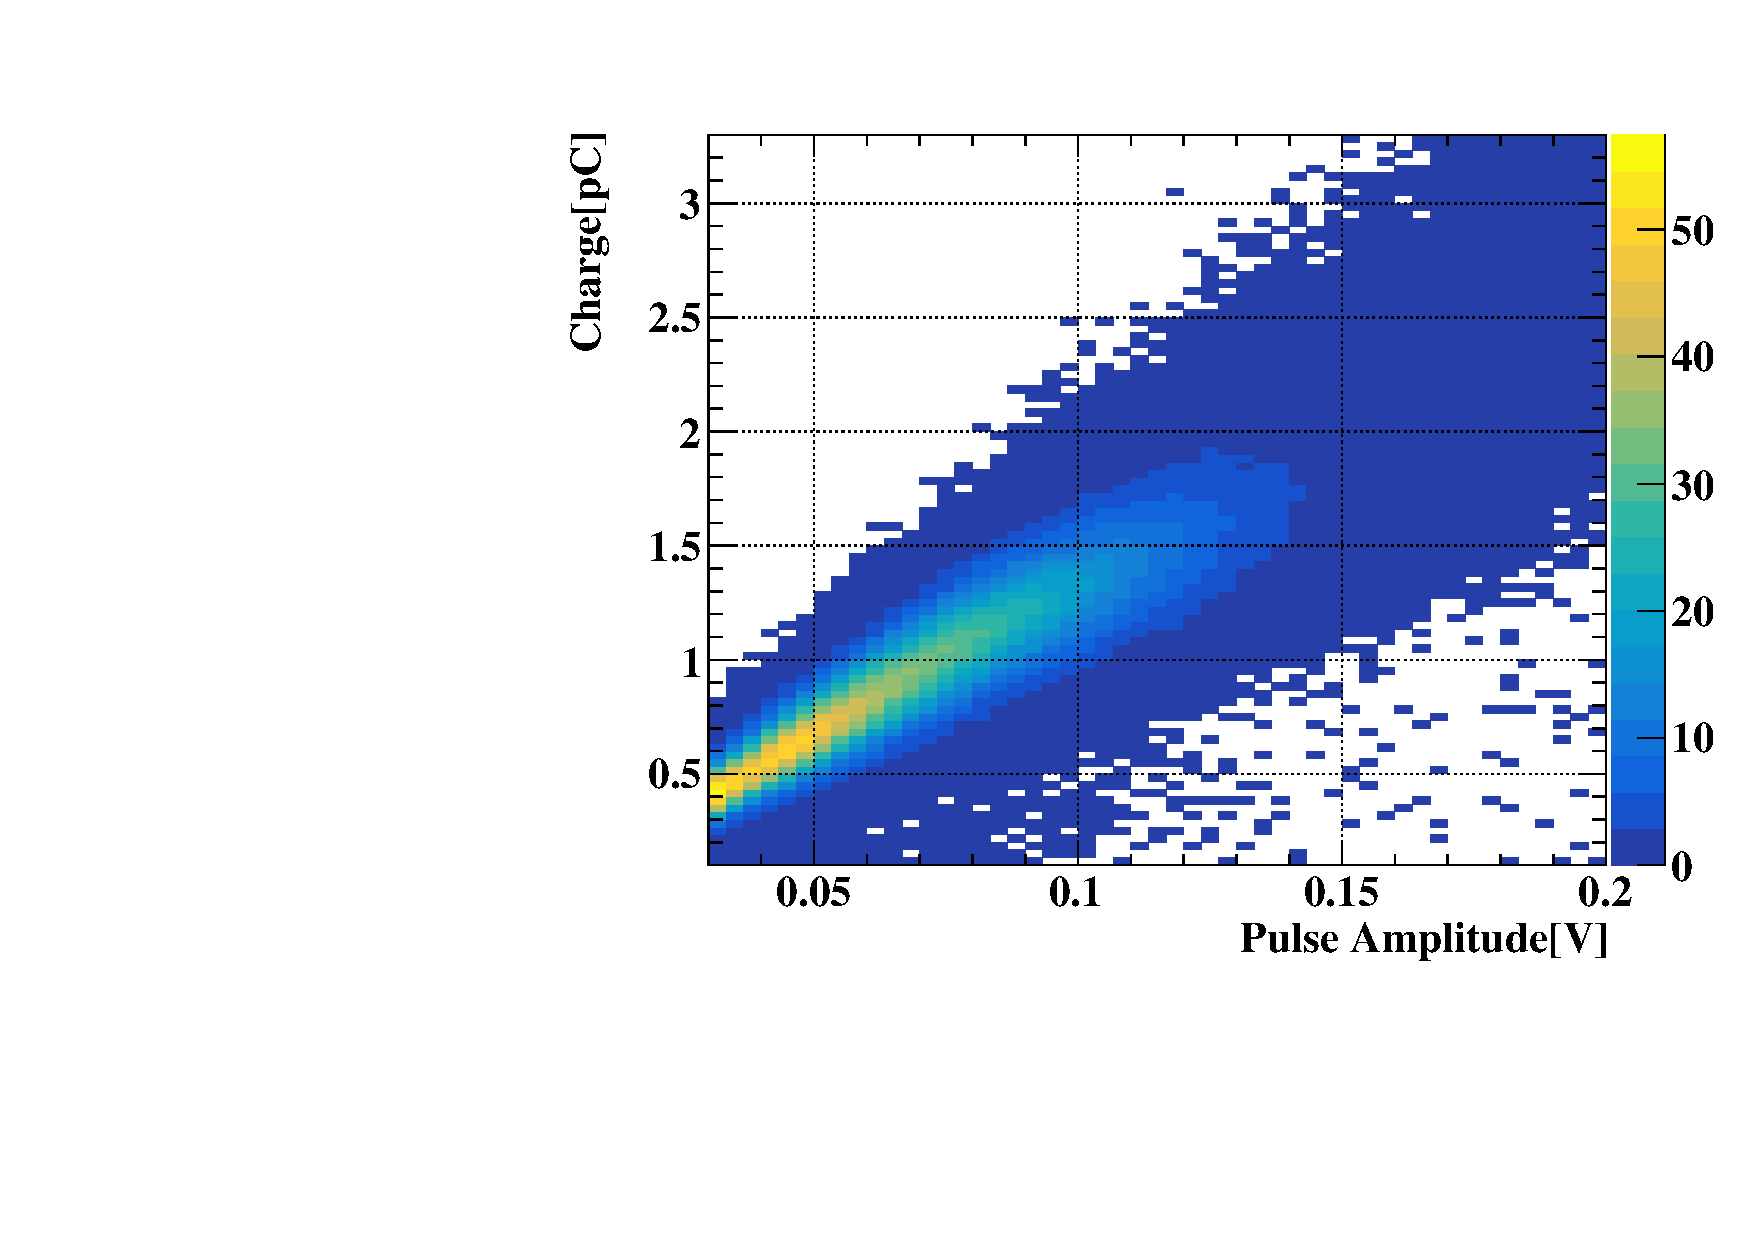
\includegraphics[width=6cm]{graphics/qvampcolor.pdf}
    \caption{Relationship of height to charge in a single event waveform, across all MPPCs}
    \label{fig:qvsamp}
\end{figure}
\begin{figure}
    \centering
    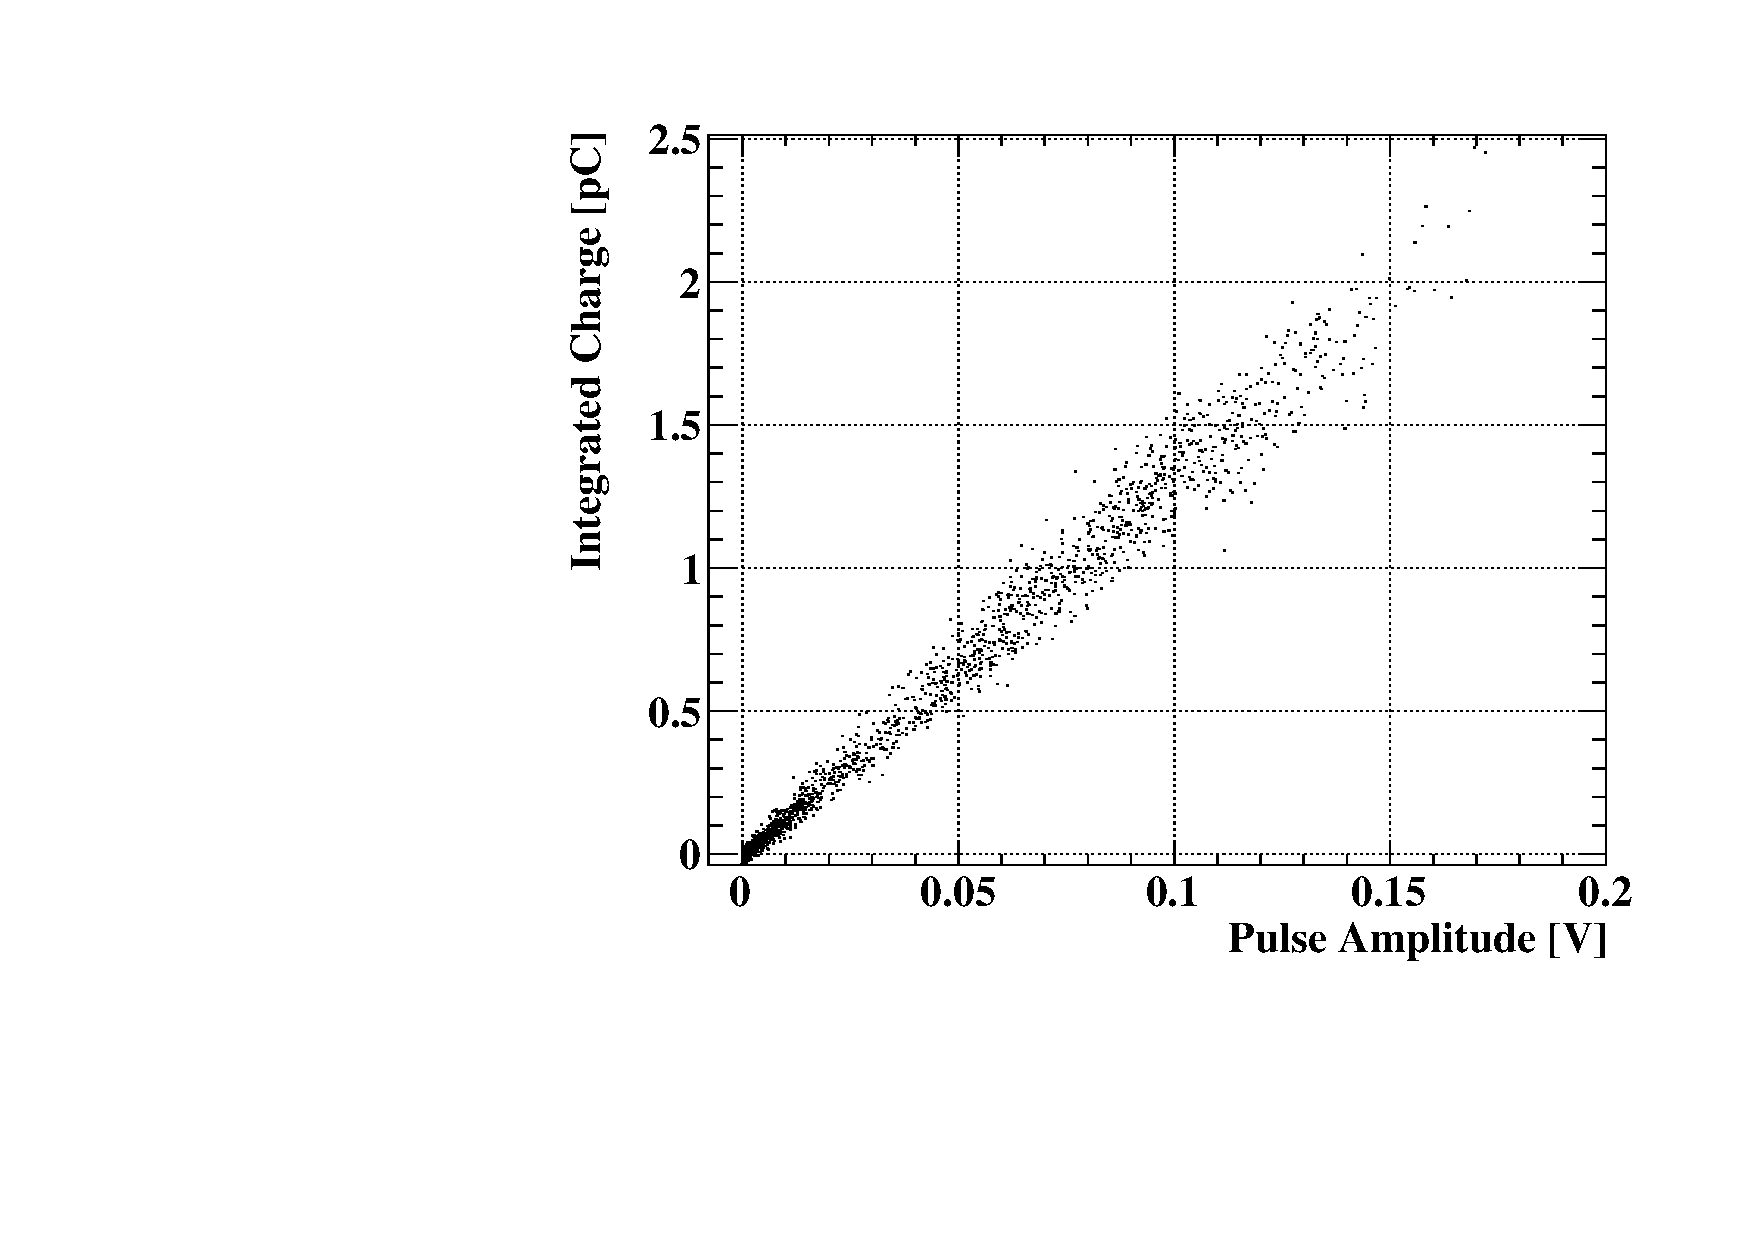
\includegraphics[width=6cm]{graphics/qvampsingle.pdf}
    \caption{Relationship of height to charge in a single event waveform, in a single MPPC}
    \label{fig:qvsampsing}
\end{figure}

Particularly of note is that there are significant differences in this relation across the face of individual MPPCs.
Figure \ref{fig:heightvzplot} shows this via the net average mppc charge and height behaviour v. position across all scanned mppcs.
From a polynomial fit of both of these figures, we find, as agrees with prior findings, that the peaks of the charge measurements agree with our previous results of a 10\% drop in the downboard half. For height, the same effect still appears but to a much lesser extent.

\begin{figure}
\centering

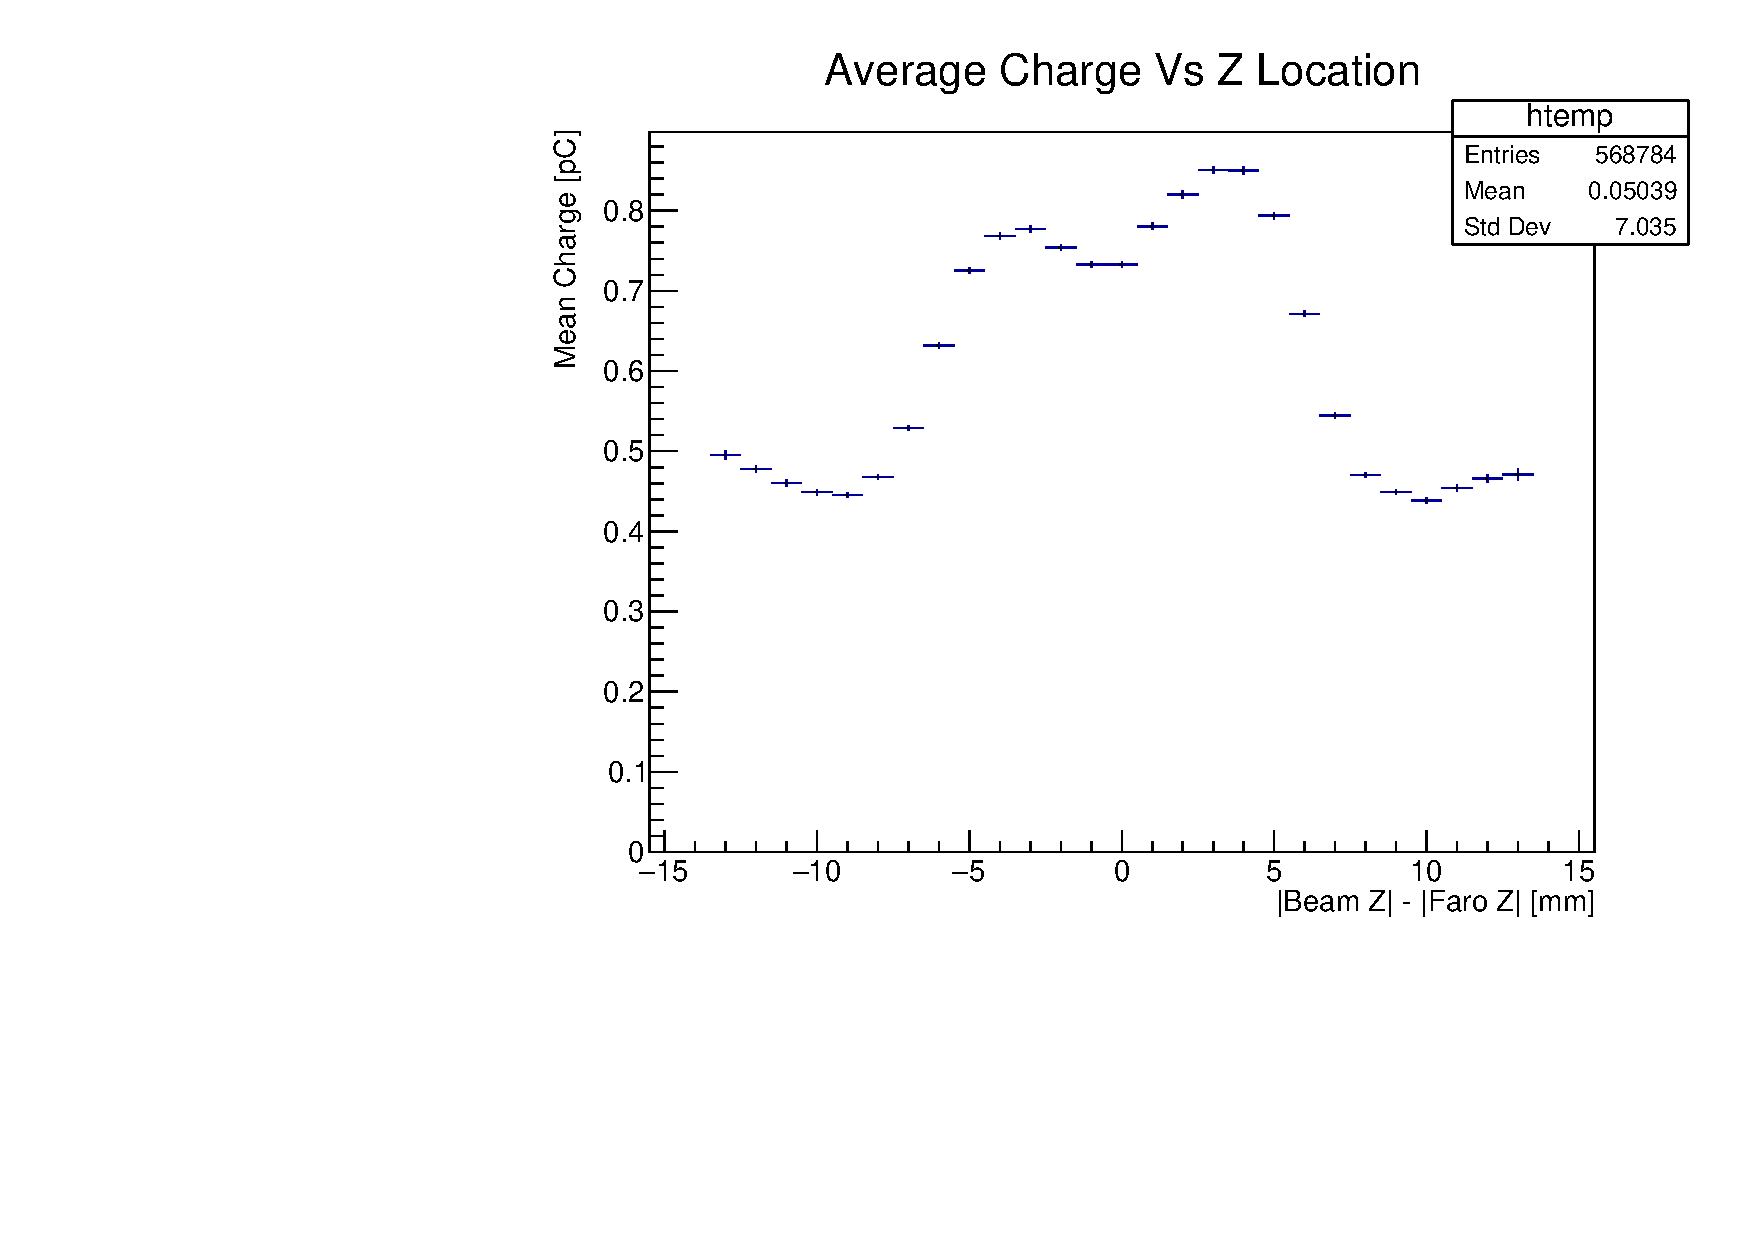
\includegraphics[width=4 cm]{graphics/chargevsz.pdf}
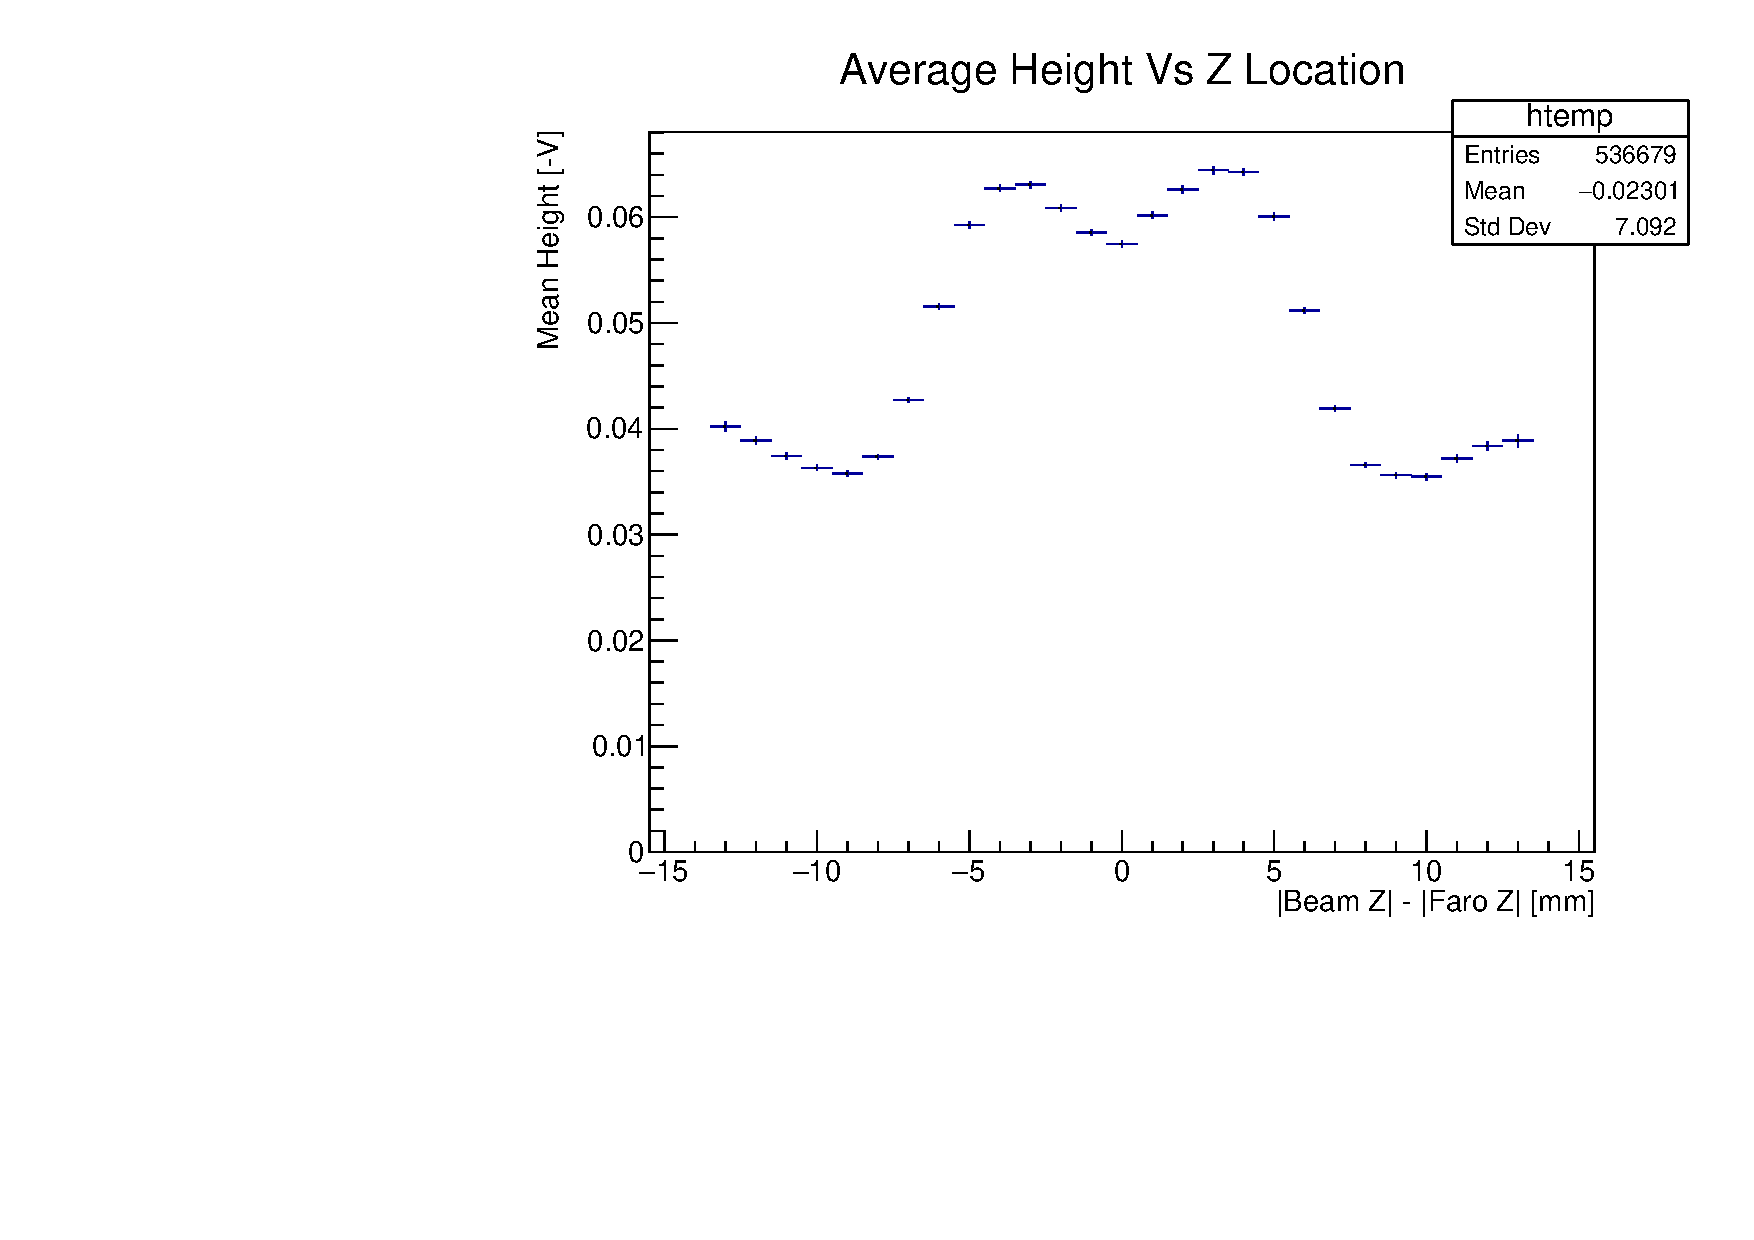
\includegraphics[width=4 cm]{graphics/heightvsz.pdf}
\caption{Average charge (left), height (right) in an event relative to measurement location on MPPC}
\label{fig:heightvzplot}
\end{figure}

\begin{figure}
\centering
    
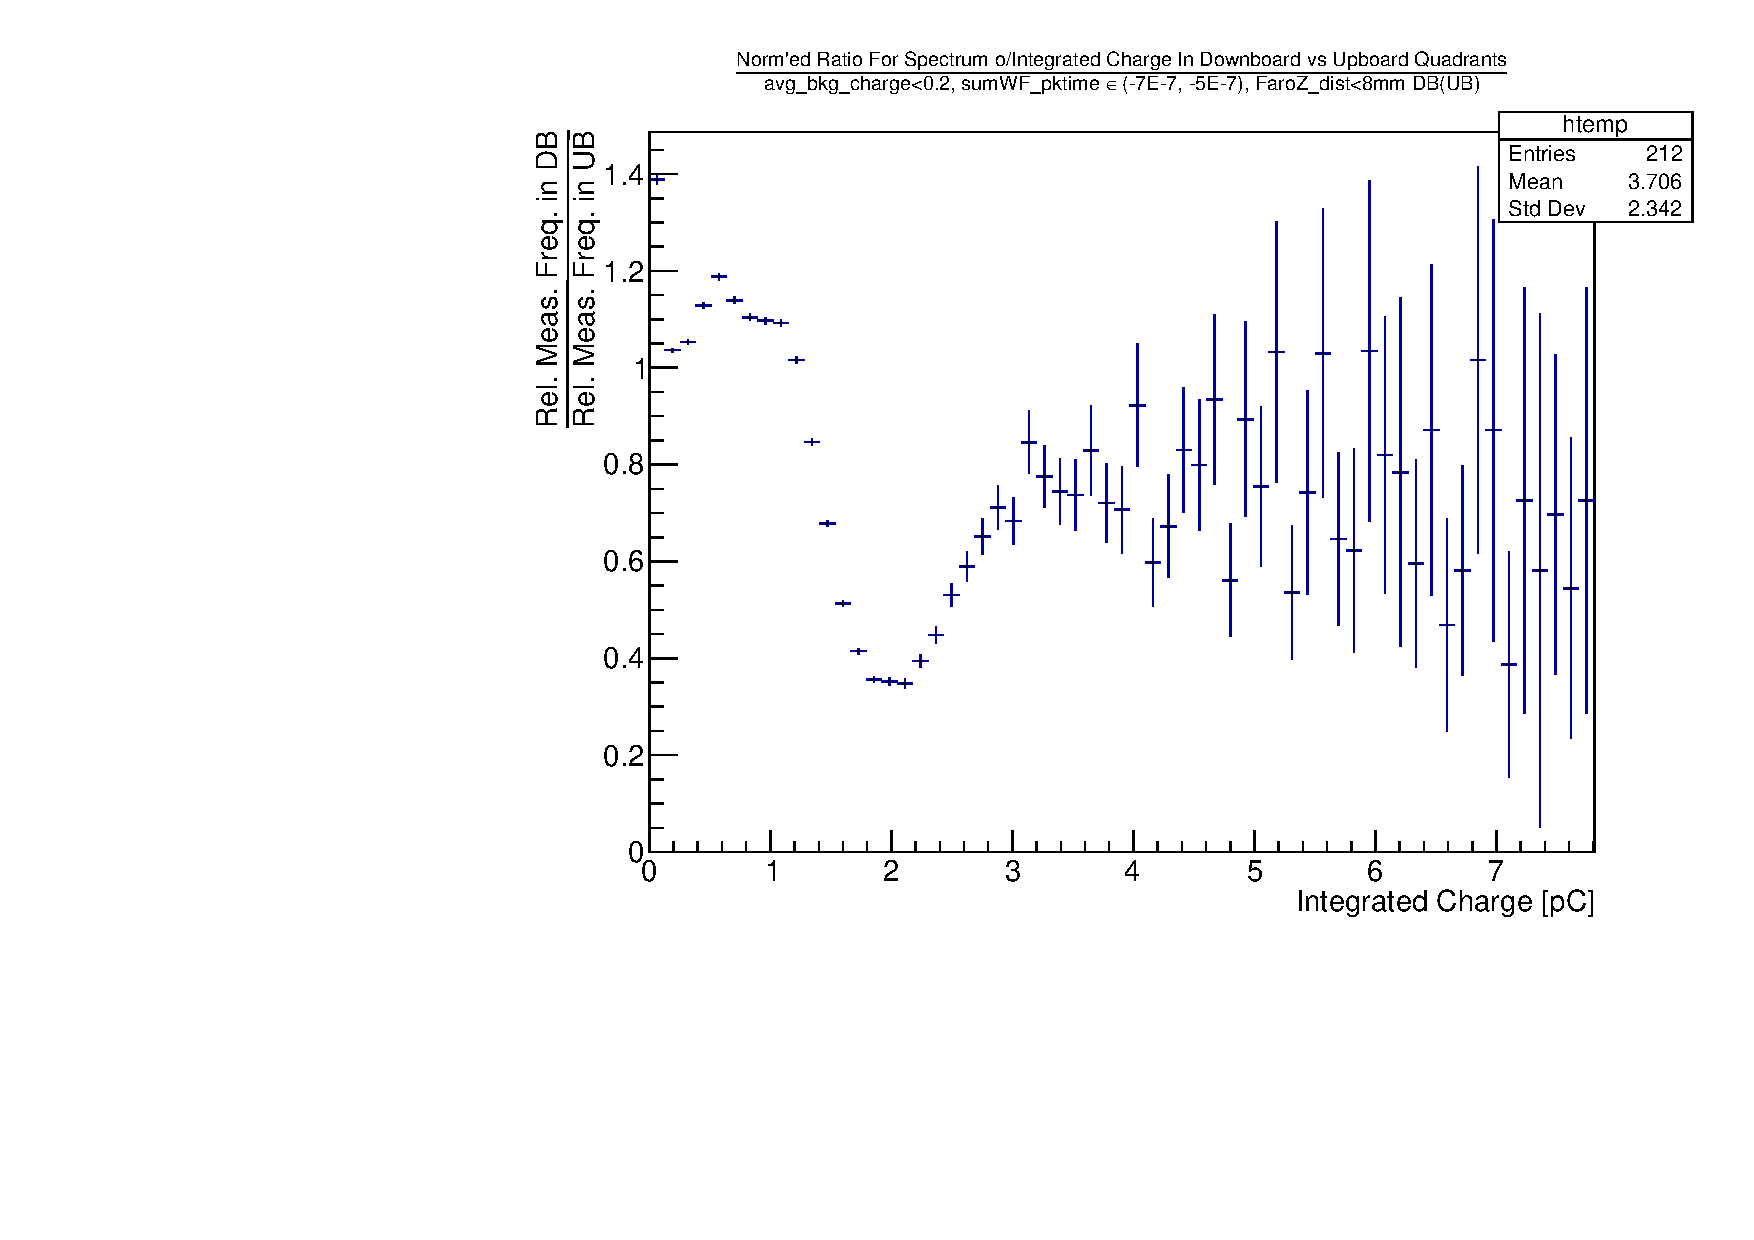
\includegraphics[width=4 cm]{graphics/chargeratiospectrum_DBtoUB.pdf}
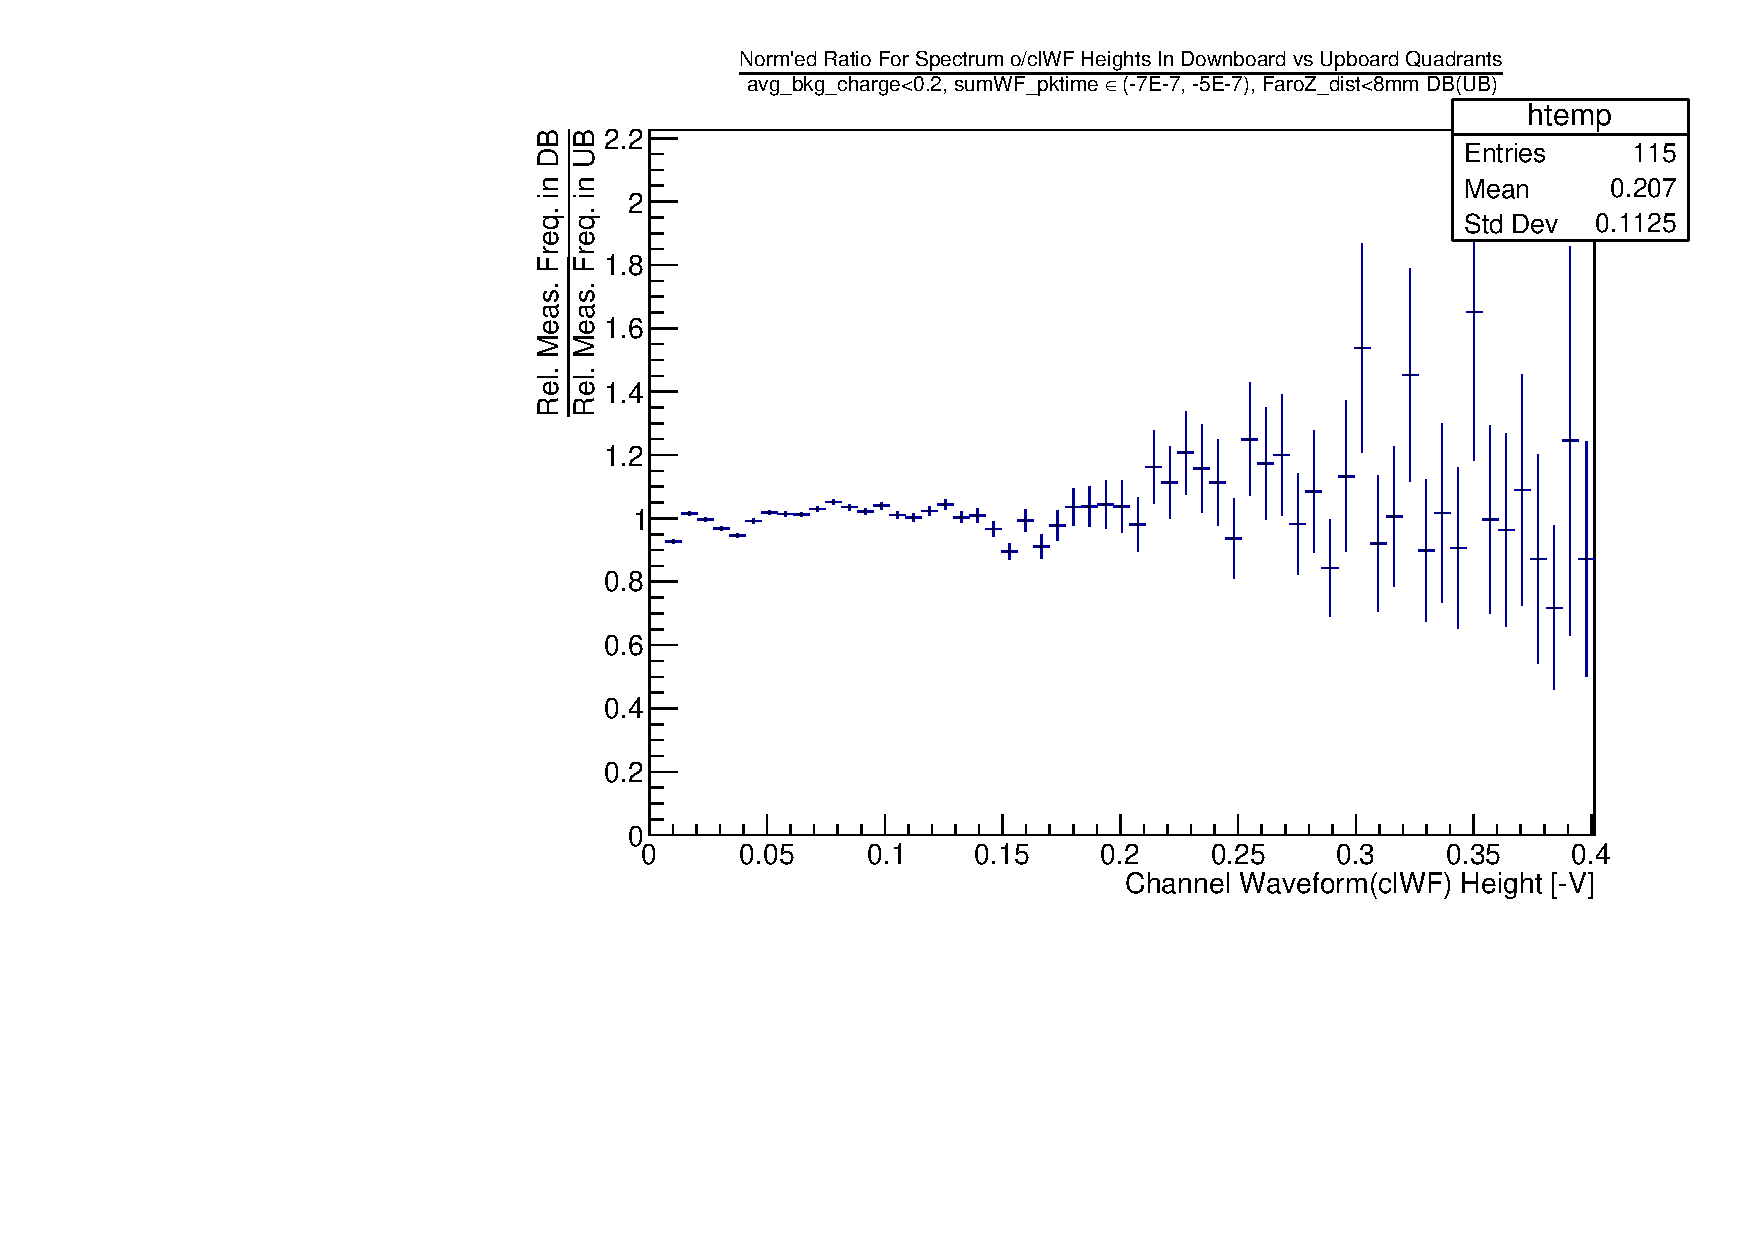
\includegraphics[width=4 cm]{graphics/heightratiospectrum_DBtoUB.pdf}
\caption{Ratio of normalized charge (left), height (right) distributions in each MPPC half}
\label{fig:heightspectrumplot}
\end{figure}

\begin{table}[H]
    \centering
    \begin{tabular}{c||c|c|c}
         & DB Peak & UB Peak & Ratio \\
         \hline
        Charge & 0.777548 pC & 0.860434 pC & 0.903669 \\
        Height & 63.336 mV & 65.0873 mV & 0.973094
    \end{tabular}
    \caption{Amplitude of Height and Charge Distributions For MPPC Halves }
    \label{tab:qandhhalves}
\end{table}




Additionally, we are interested in the relative response between the two MPPC halves across the range of charge and height measurements.
Figure \ref{fig:heightspectrumplot} is especially interesting because these plots allow us to determine the differential nature in which the two sides will be effected by any alterations to the chosen threshold value. In the region of our selection criteria, the charge threshold will reject a higher number of events on the side closer to Z=0, whereas a selection on height effect both sides of the mppc equally. Moreover, this shift is in fact confirmed when we analyze the found mppc positions from both cuts, where a clear shift outwards from zero is present in the charge based cuts (Fig. \ref{fig:seldzvz}).
\begin{figure}
    \centering
    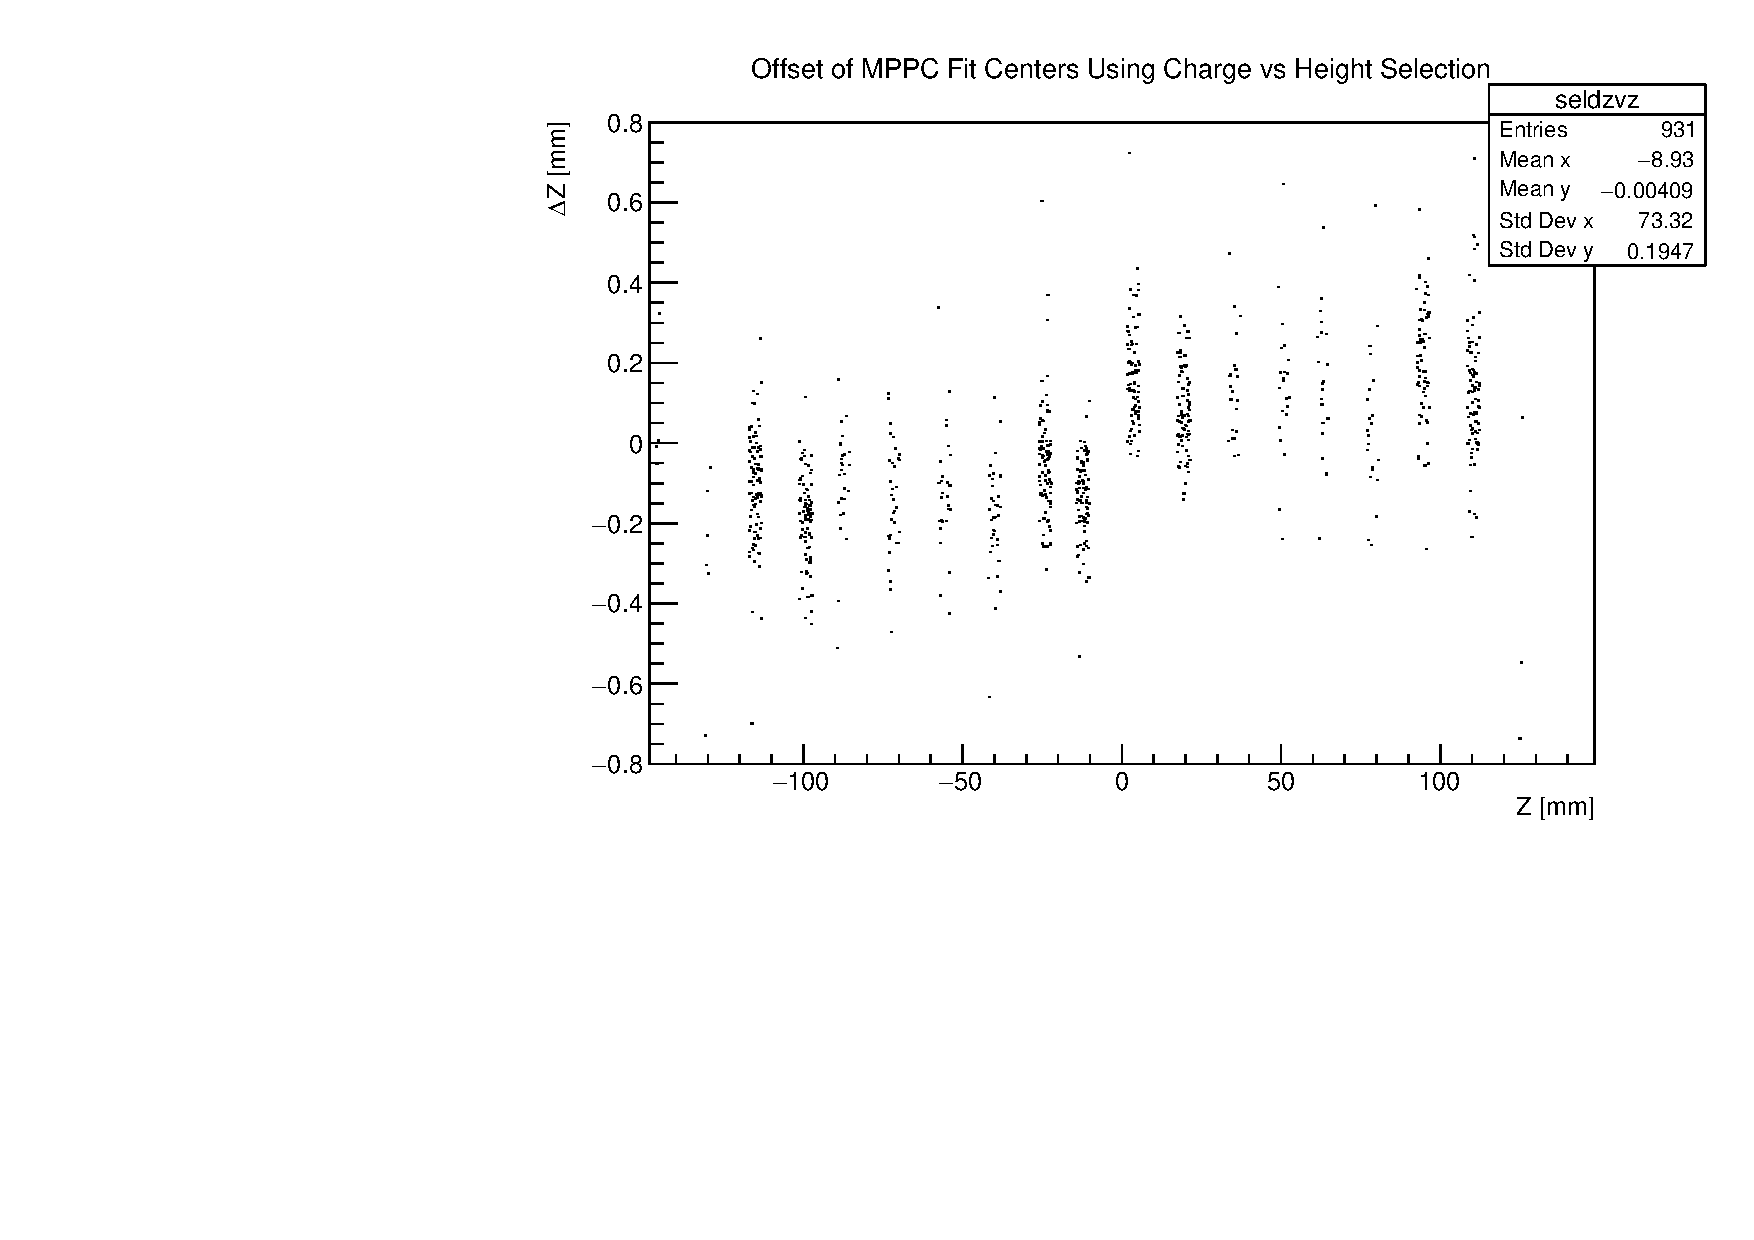
\includegraphics[width=5cm]{graphics/selectionshiftoverz.pdf}
    \caption{Difference in found positions under change from charge to amplitude selection}
    \label{fig:seldzvz}
\end{figure}

\begin{table}[H]
    \caption{Integrated charge based selection criteria. Criteria are, $Q_{cl}$: charge of channel waveform; $T_{pk}$: time of peak in sum trigger waveform; $\left<Q_{bkg}\right>$: Mean charge in negative trigger channels}
    \label{tab:qselcrit}
    \centering
    \begin{tabular}{l|l}
    Criterion & Value \\
    \hline
         $Q_{cl}$ & $>$ 0.6 pC \\
         $T_{pk}$ & (-0.7 $\mu s$,-0.5 $\mu s$) \\ 
         $\left<Q_{bkg}\right>$ & $<$ 0.2 pC
    \end{tabular}
    
\end{table}
\begin{table}[H]
    \caption{Pulse Amplitude based selection criteria. Criteria are, $A_{cl}$: pulse amplitude of channel waveform; $T_{pk}$: time of peak in sum trigger waveform; $\left<Q_{bkg}\right>$: Mean charge in negative trigger channels}
    \label{tab:ampselcrit}
    \centering
    \begin{tabular}{l|l}
    Criterion & Value \\
    \hline
         $A_{cl}$ & $>$ 0.6 pC \\
         $T_{pk}$ & (-0.7 $\mu s$,-0.5 $\mu s$) \\ 
         $\left<Q_{bkg}\right>$ & $<$ 0.2 pC
    \end{tabular}
    
\end{table}

All charge values are gain corrected by direct measurement or by measured mean of production lot if direct measurement isn't possible.


\textbf{Stability Under Variation of Thresholds}\\
As follows, we observe that there is no introduced dependency of the found MPPC locations on our chosen values of selection threshold for either of the charge and height based selection schemes. Using the found MPPC spacing as our metric for comparison, the supergaussian fit procedure was used to analyze all data runs at a range of cut thresholds with the results being shown in Fig. \ref{tab:spacingqthres} and \ref{tab:spacingampthres}.

\begin{table}
    \centering
    \begin{tabular}{c|cc|cc}
        Cut &Odd  $n$&Std. Dev.&Even  $n$&Std. Dev.\\
        \text{[pC]}&[mm]&[mm]&[mm]&[mm]\\
        \hline
        0.4 & 14.82(2) & 0.331(12) & 15.23(4) & 0.434(35) \\ 
        0.5 & 15.00(1) & 0.254(8) & 15.16(2) & 0.279(22) \\ 
        0.6 & 15.10(1) & 0.225(9) & 15.08(2) & 0.234(16) \\ 
        0.7 & 15.11(1) & 0.211(7) & 15.09(2) & 0.217(16) \\ 
        0.8 & 15.11(1) & 0.244(10) & 15.08(2) & 0.233(25) \\ 
    \end{tabular}
    \caption{Spacing of adjacent MPPCs using different cut values on integrated charge}
    \label{tab:spacingqthres}
\end{table}
\begin{table}
    \centering
    \begin{tabular}{c|cc|cc}
        Cut &Odd  $n$&Std. Dev.&Even  $n$&Std. Dev.\\
        \text{[mV]}&[mm]&[mm]&[mm]&[mm]\\
        \hline
        40 & 15.09(1) & 0.226(7) & 15.05(2) & 0.213(14) \\ 
        50 & 15.13(1) & 0.221(8) & 15.04(1) & 0.188(13) \\ 
        60 & 15.10(1) & 0.221(8) & 15.07(2) & 0.191(16) \\ 
    \end{tabular}
    \caption{Spacing of adjacent MPPCs using different cut values on pulse amplitude}
    \label{tab:spacingampthres}
\end{table}


\section{Alternate Fit Function}\label{app:fitfunccomp}
The set of well fit MPPCs were selected using the following critia,
\begin{enumerate}
    \item Uncertainty In Fit Mean $<$ 0.3 mm [Z], 0.03 deg [$\phi$]
    \item Uncertainty In Fit Sigma $<$ 0.3 mm [Z], 0.03 deg [$\phi$]
    \item Fit Sigma $\in$ (5.5mm, 8.5mm)[Z], (0.4deg, 0.8deg)[$\phi$]
    \item Reduced $\chi ^{2} \; <$ 100
\end{enumerate}

Comparing this set to the found positions from the piece-wise fit function, we find the distribution contains very small offsets

\begin{figure}[h]

    \centering
    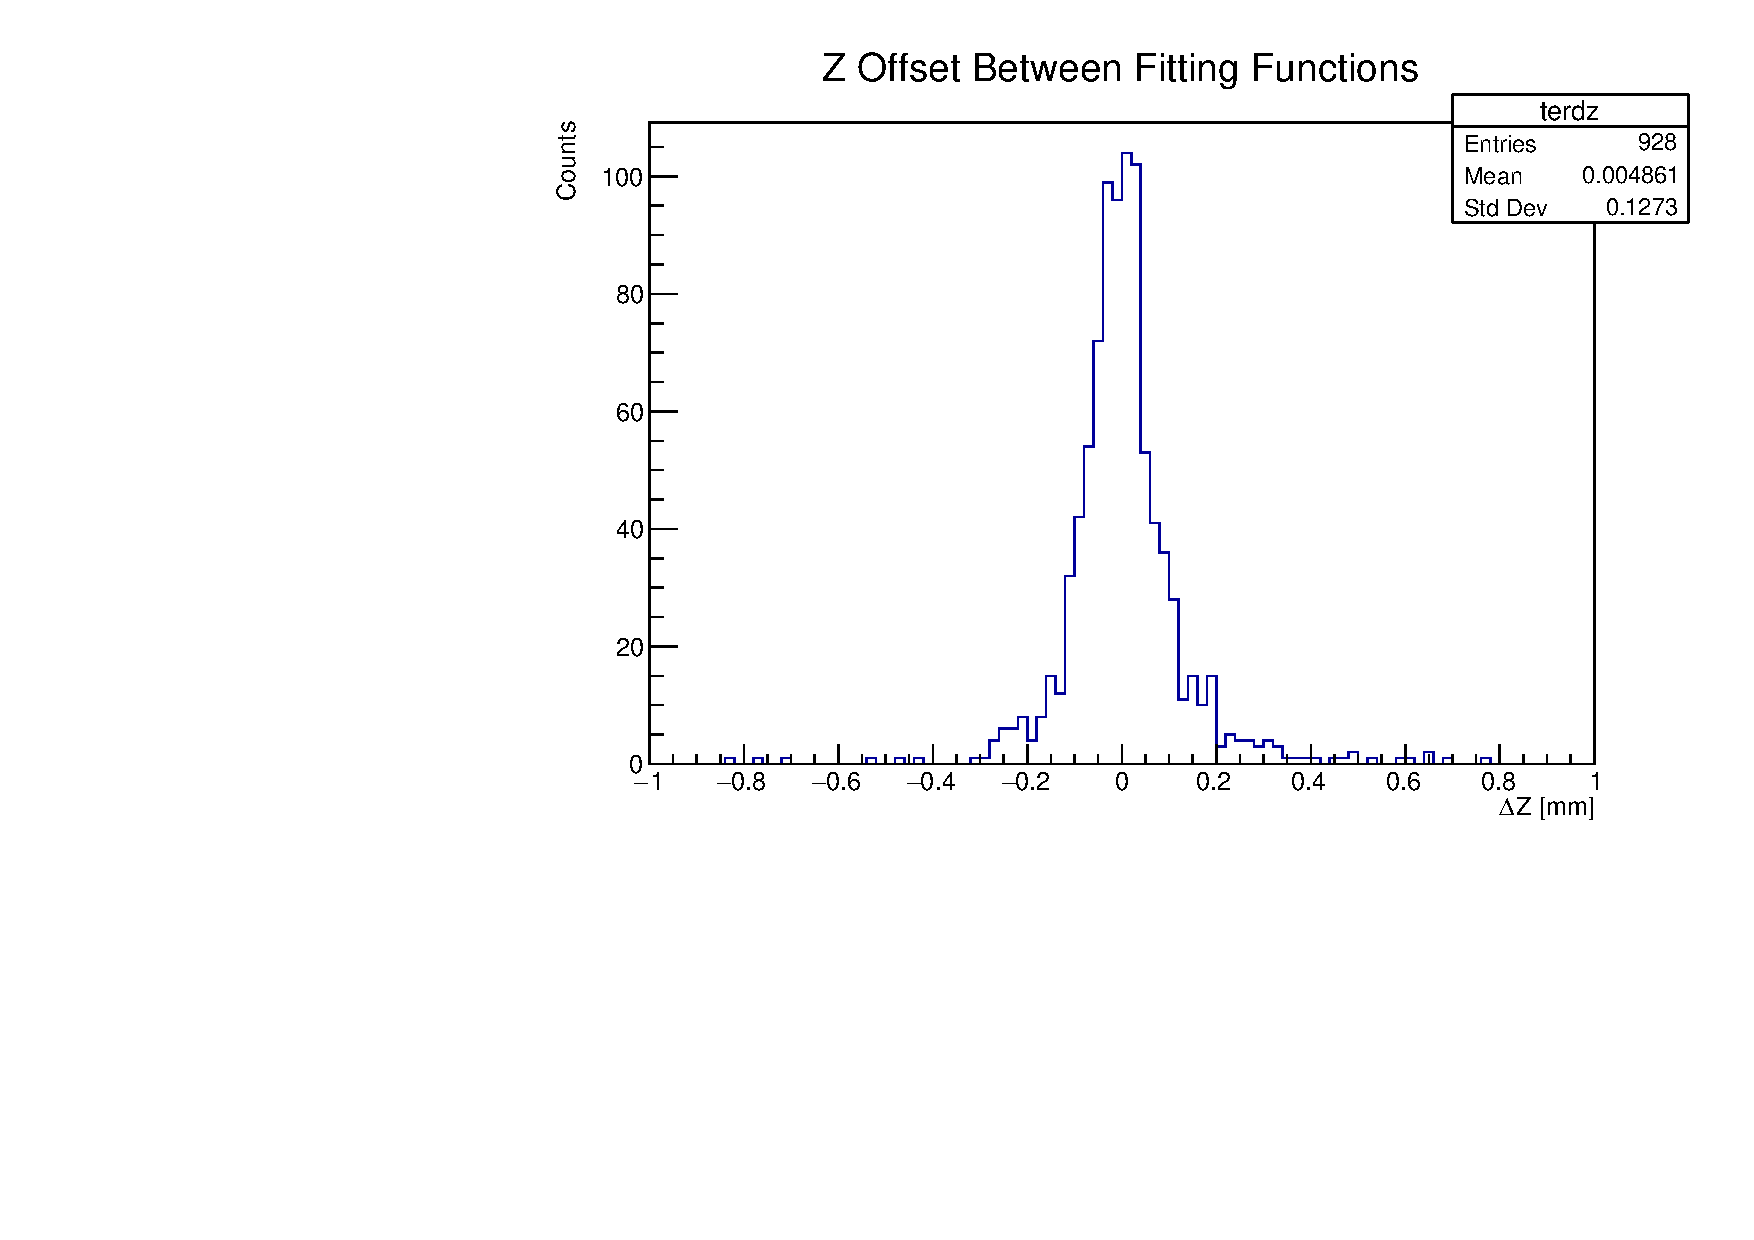
\includegraphics[width=.7\linewidth]{graphics/terdzhc.pdf}
    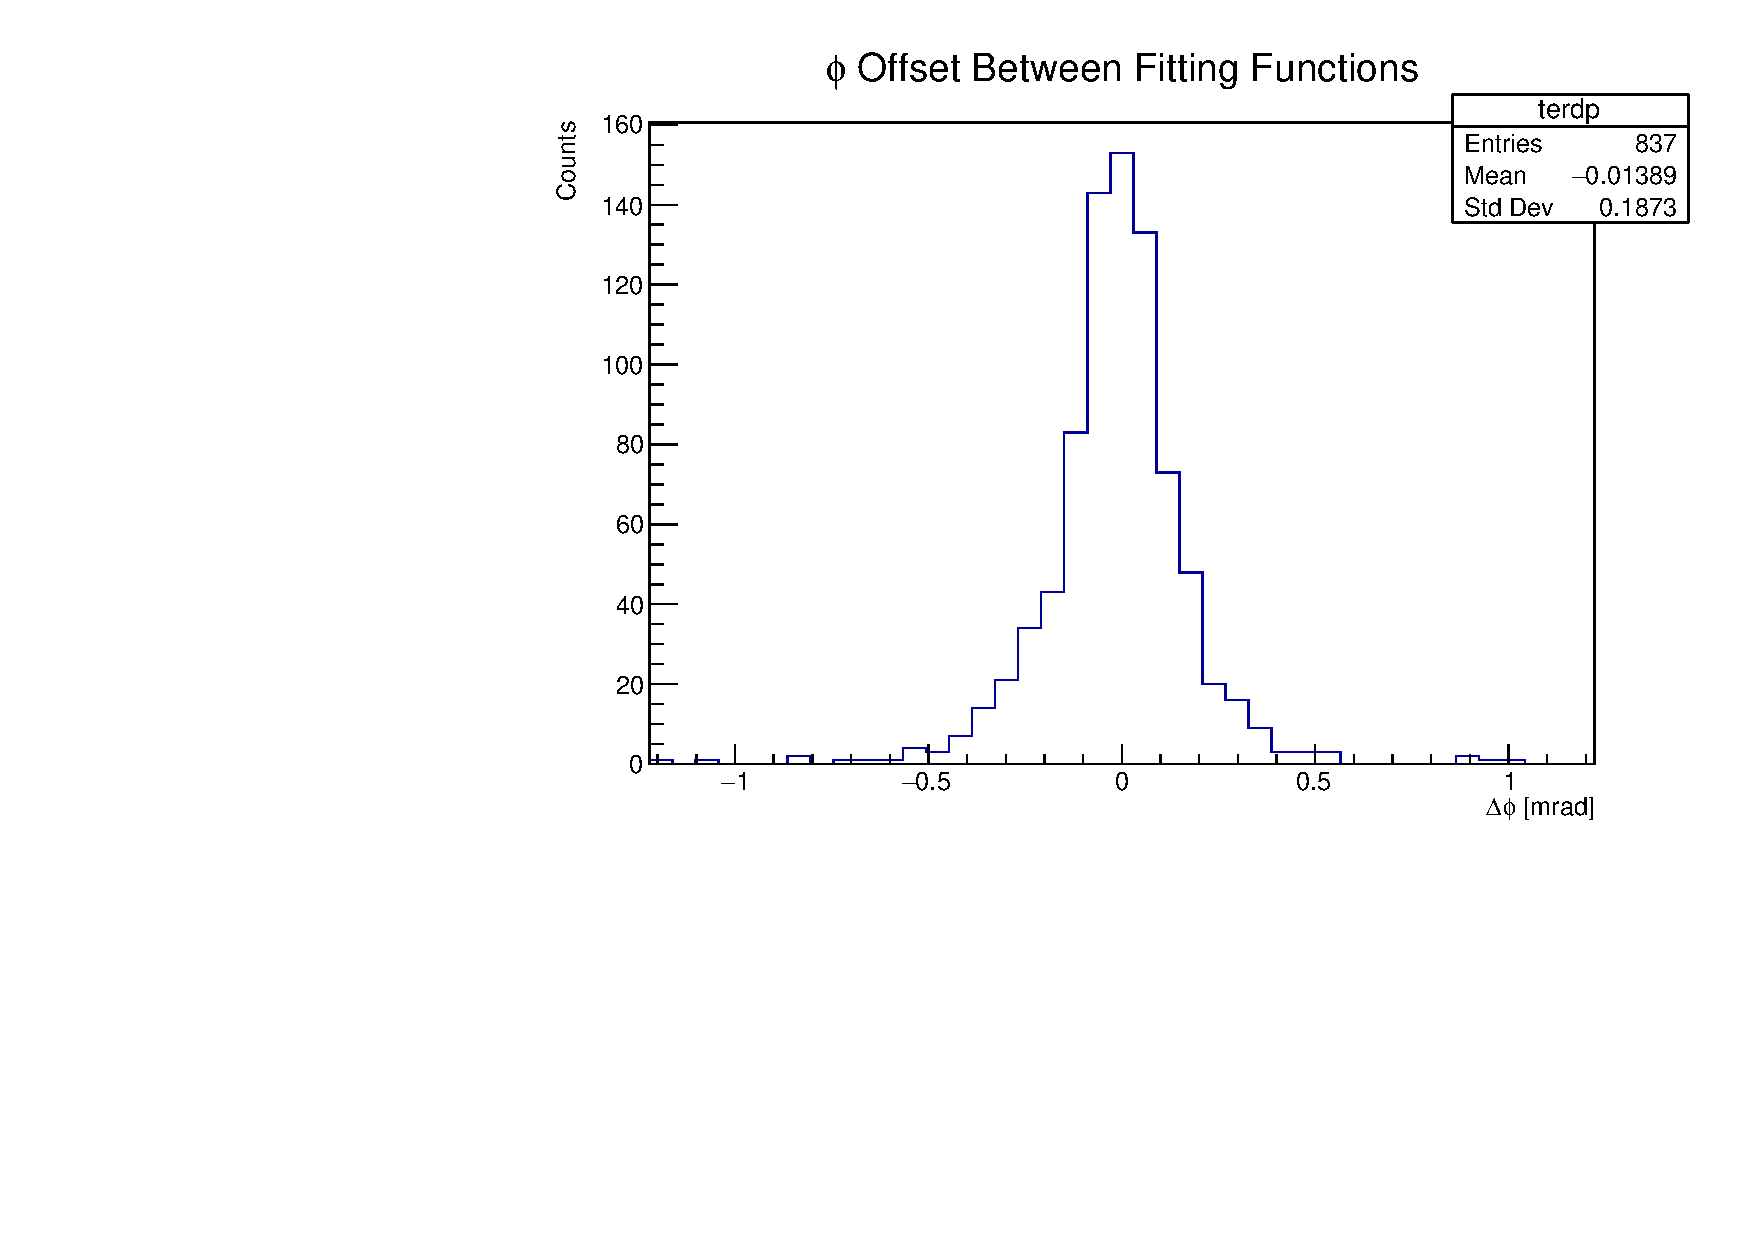
\includegraphics[width=.7\linewidth]{graphics/terdphc.pdf}
    \caption{Agreement In Found Z (top) and $\phi$ (bottom) Locations Between Fits}
    \label{fig:fitcompare}
\end{figure}


\section {X-ray Event Selection}\label{app:selection}
The X-ray events are selected using
the integrated charge, waveform amplitude and
timing, calculated over the scanned 
and background regions.
The selection criteria and the distribution of variables are given below. 
\begin{enumerate}
\item Time Waveform Peak: $-700 < T_{peak} <-500$ ns
\item Sum charge: $\Sigma Q<$1.5 pC
\item Mean background charge: $\bar{Q}_{bkg}<$0.2 pC, with either 4 or 8 background channels
\item Waveform Amplitude: $A_i>$50 mV. 
\end{enumerate}
\begin{figure}[h]
    \centering
    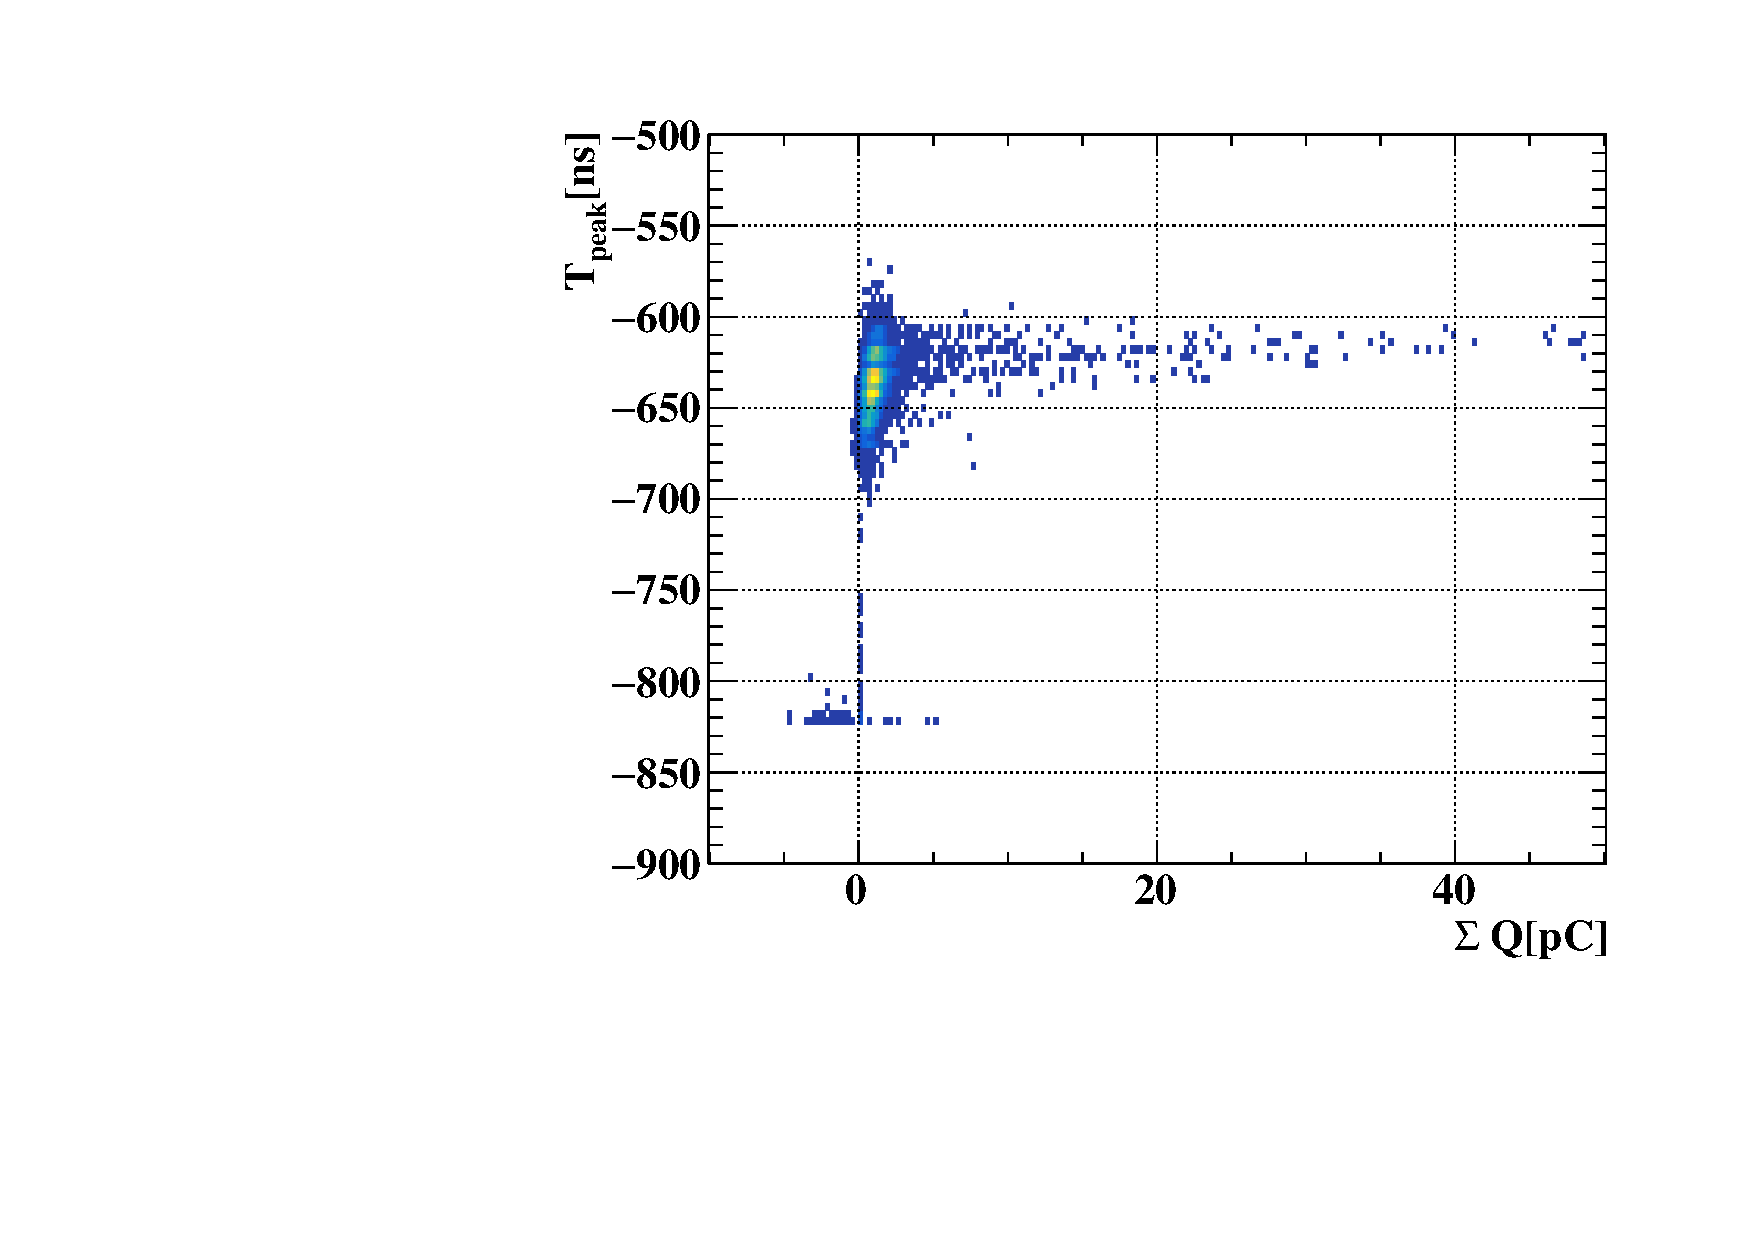
\includegraphics[width=.4\linewidth]{plots/2018/Sel1}
    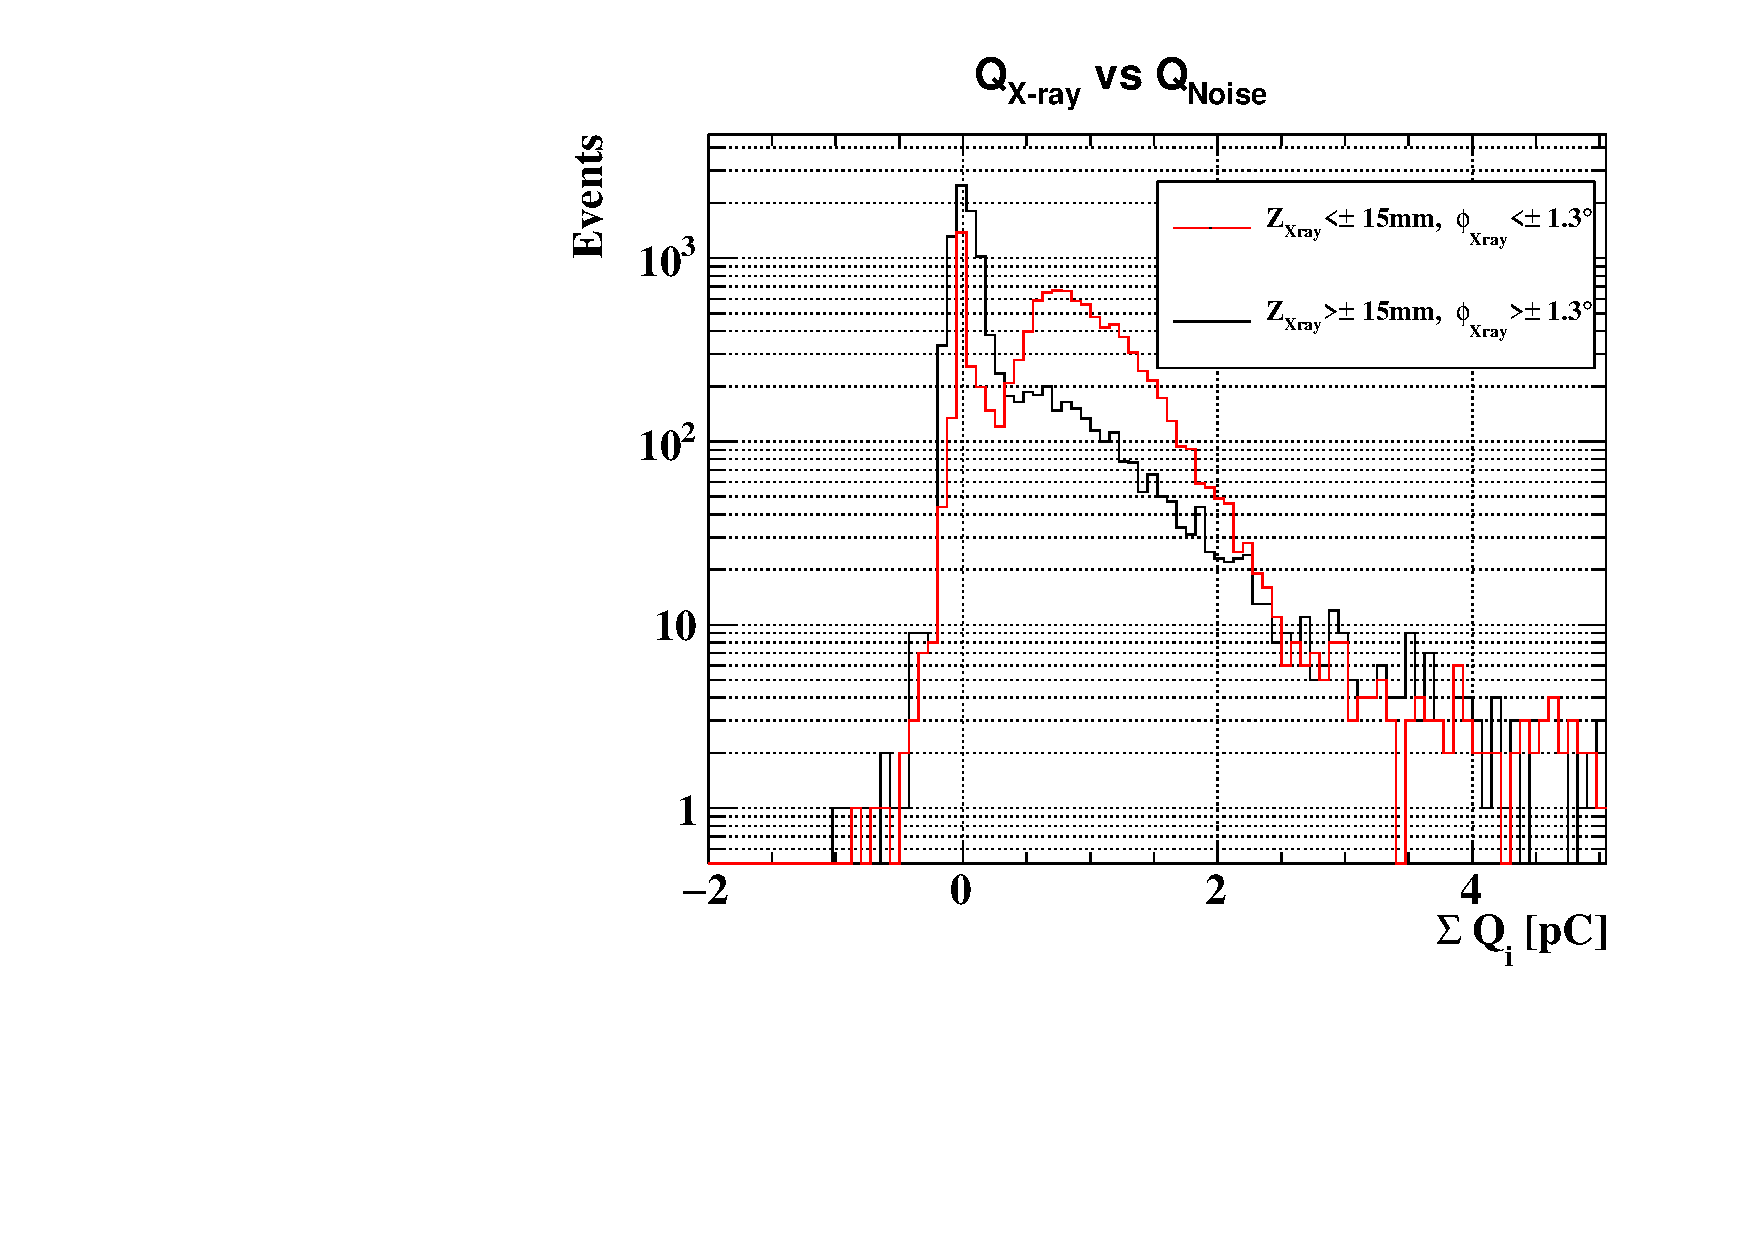
\includegraphics[width=.4\linewidth]{plots/2018/Sel2}\\
    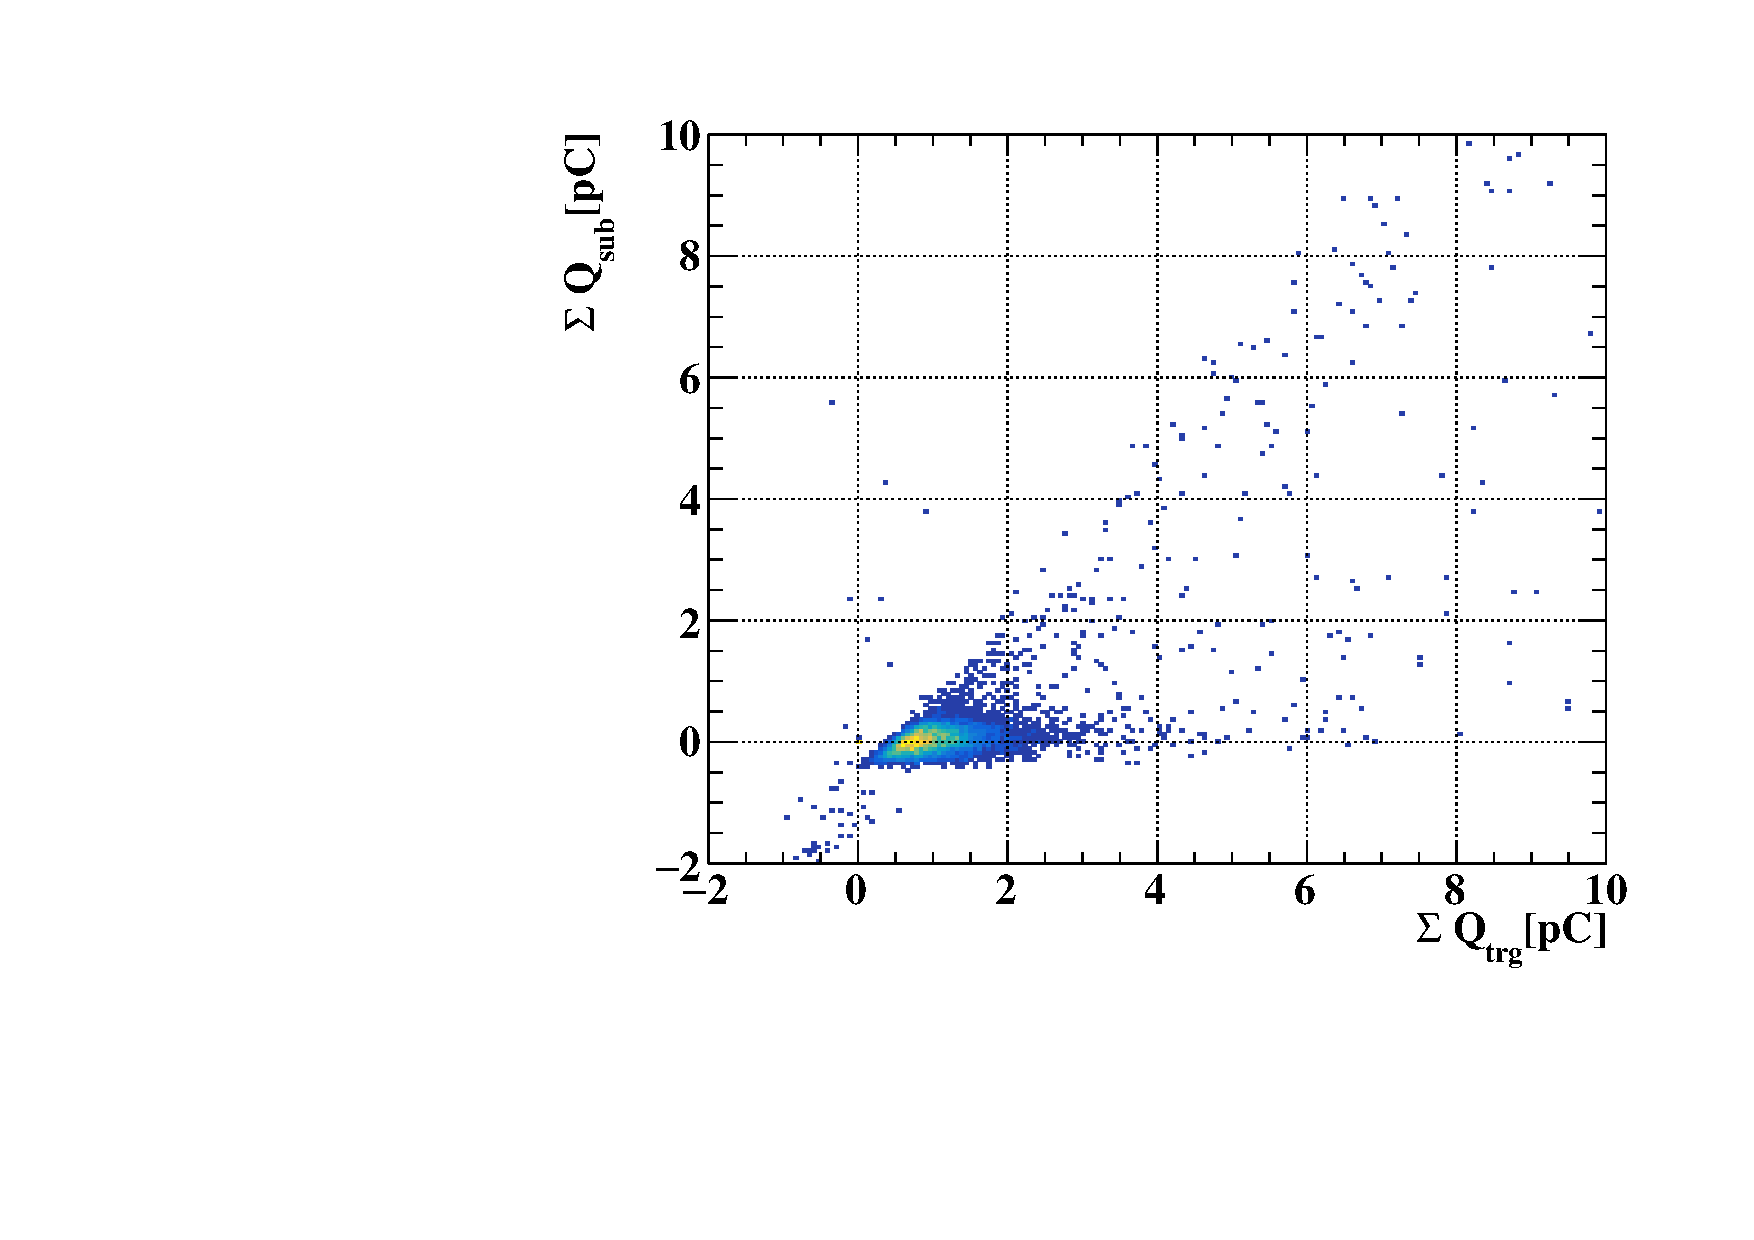
\includegraphics[width=.4\linewidth]{plots/2018/Sel3}
    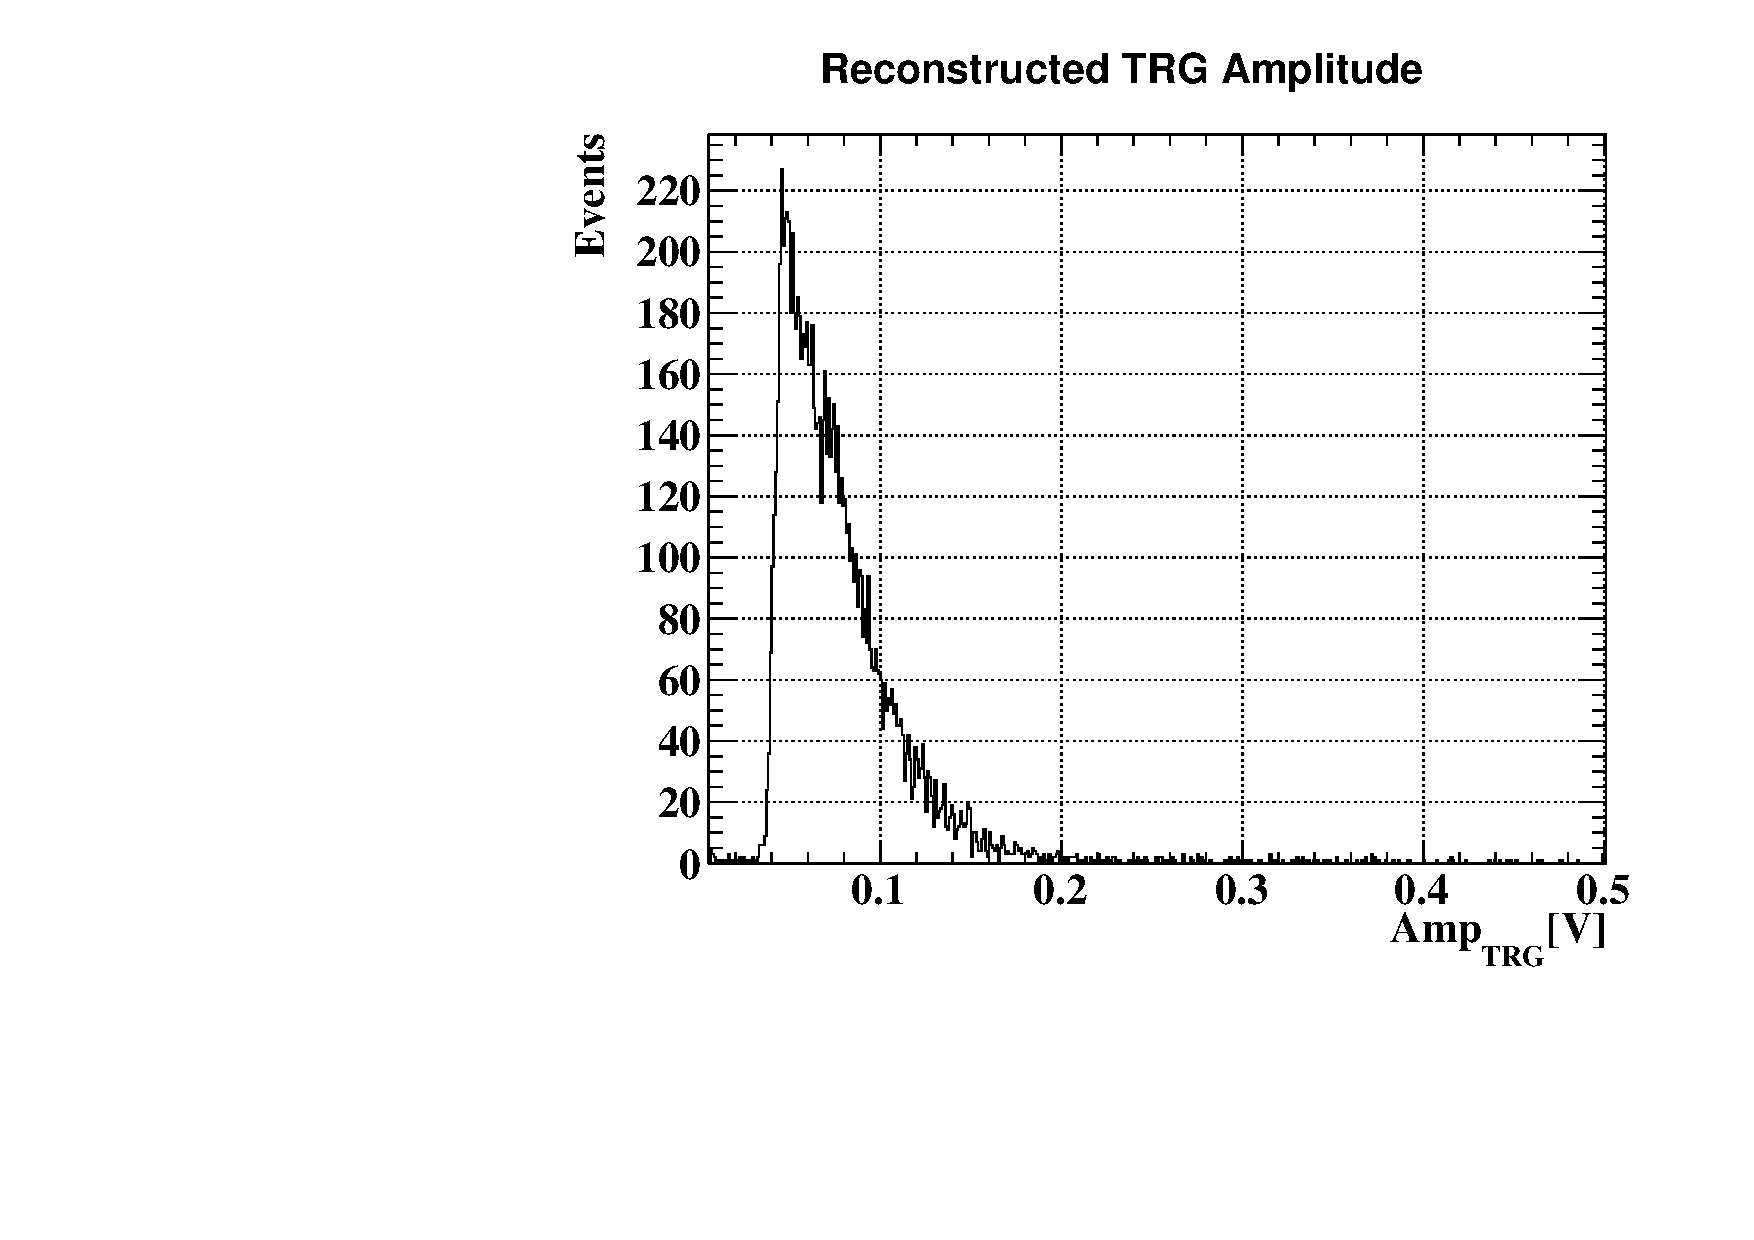
\includegraphics[width=.4\linewidth]{plots/2018/Sel4}
  \label{fig:selectionvariables}
  \caption{Variables used for X-ray event selection.}
\end{figure}

The left and right halves of the photodetector along the $\hat{z}$ direction
show different response to the X-ray signal (Sec.\ref{sec:qegain}).  In fig.
\ref{fig:mppcleftright} the mean charge and waveform amplitude are calculated
from the entire dataset, showing disparity in both observables; 
greater in charge (10\%) than in waveform amplitude(3\%). 
As a result, the reconstructed positions using the two criteria are 
displaced with respect to each other. Since the polarity of left-right
response changes about the center line (Z = 0 mm), the direction of
displacement also changes correspondingly (fig. \ref{fig:chargevswfamp}).

\begin{figure}[h]
    \centering
    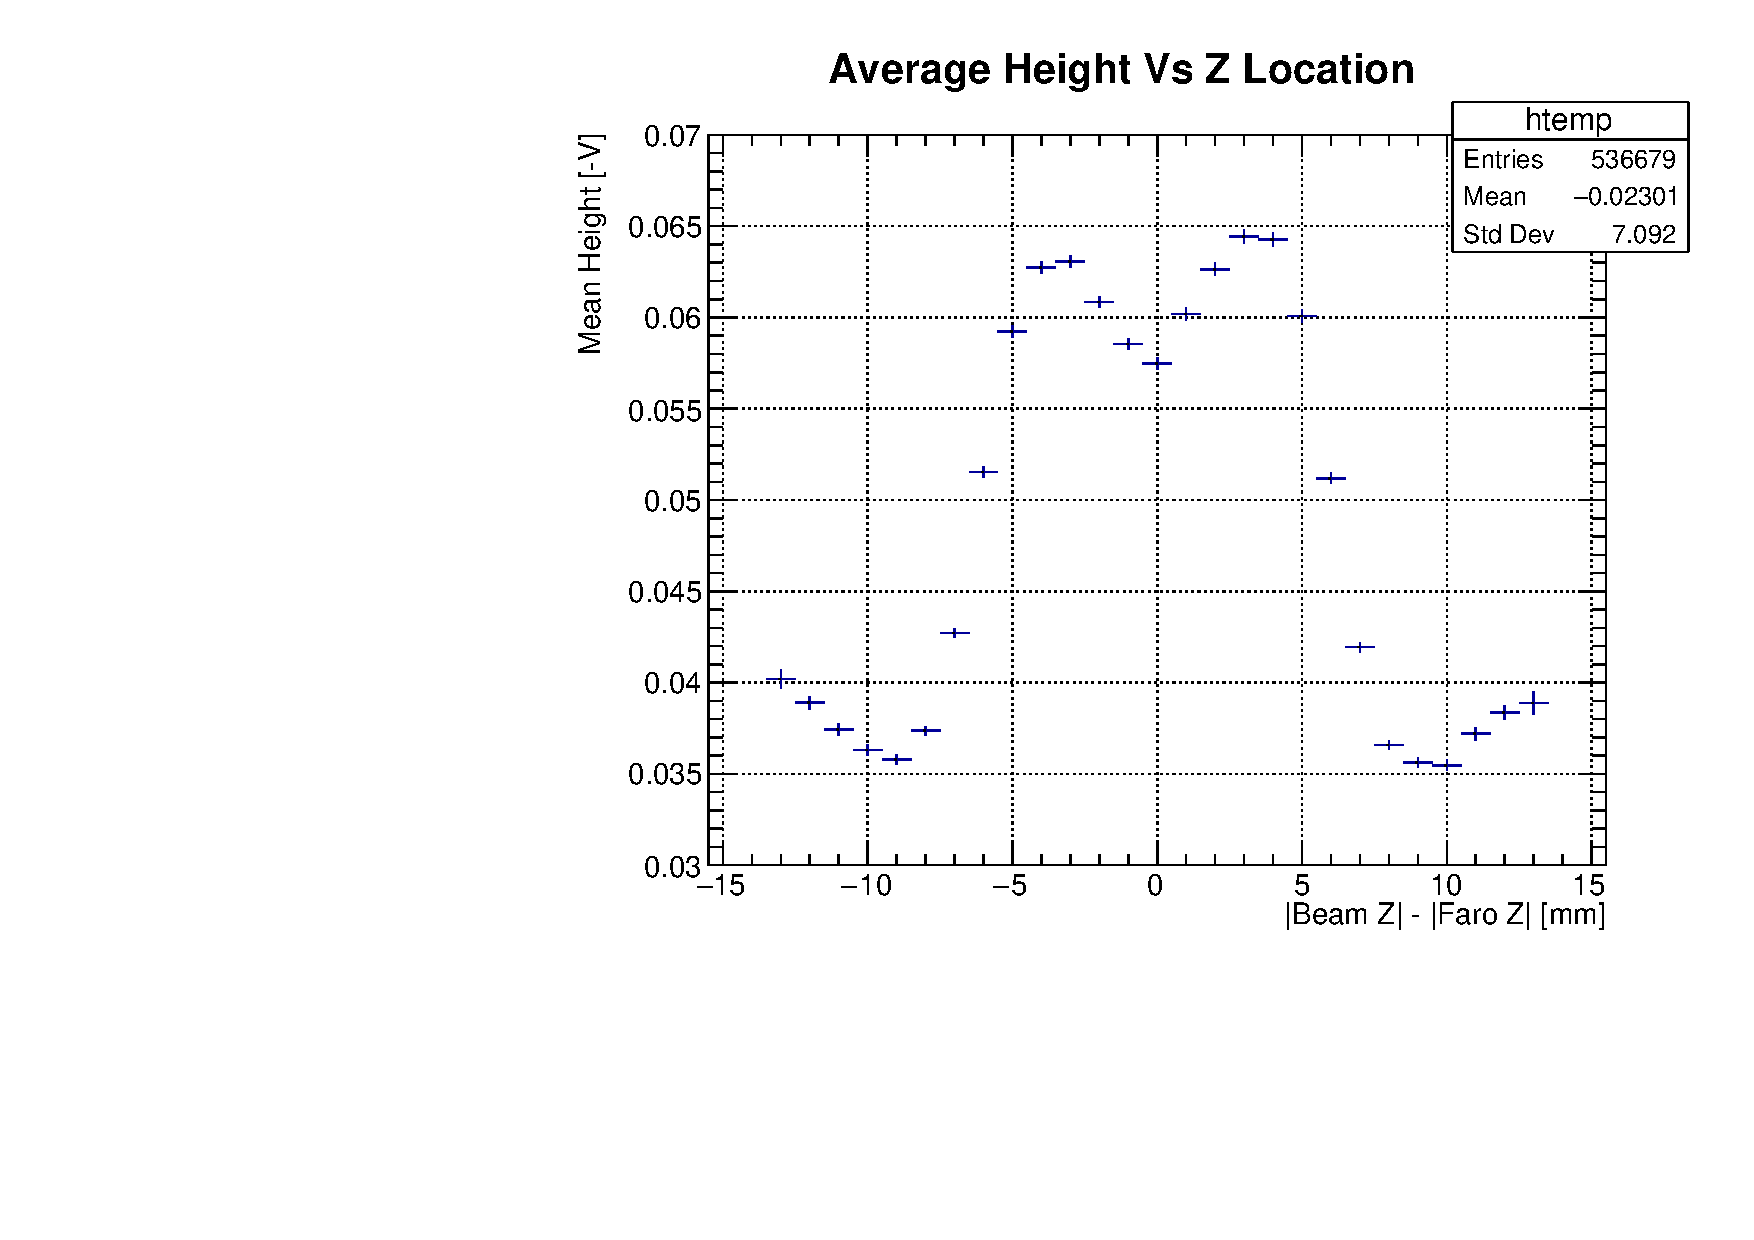
\includegraphics[width=.4\linewidth]{plots/2018/HeightvsZ2}
    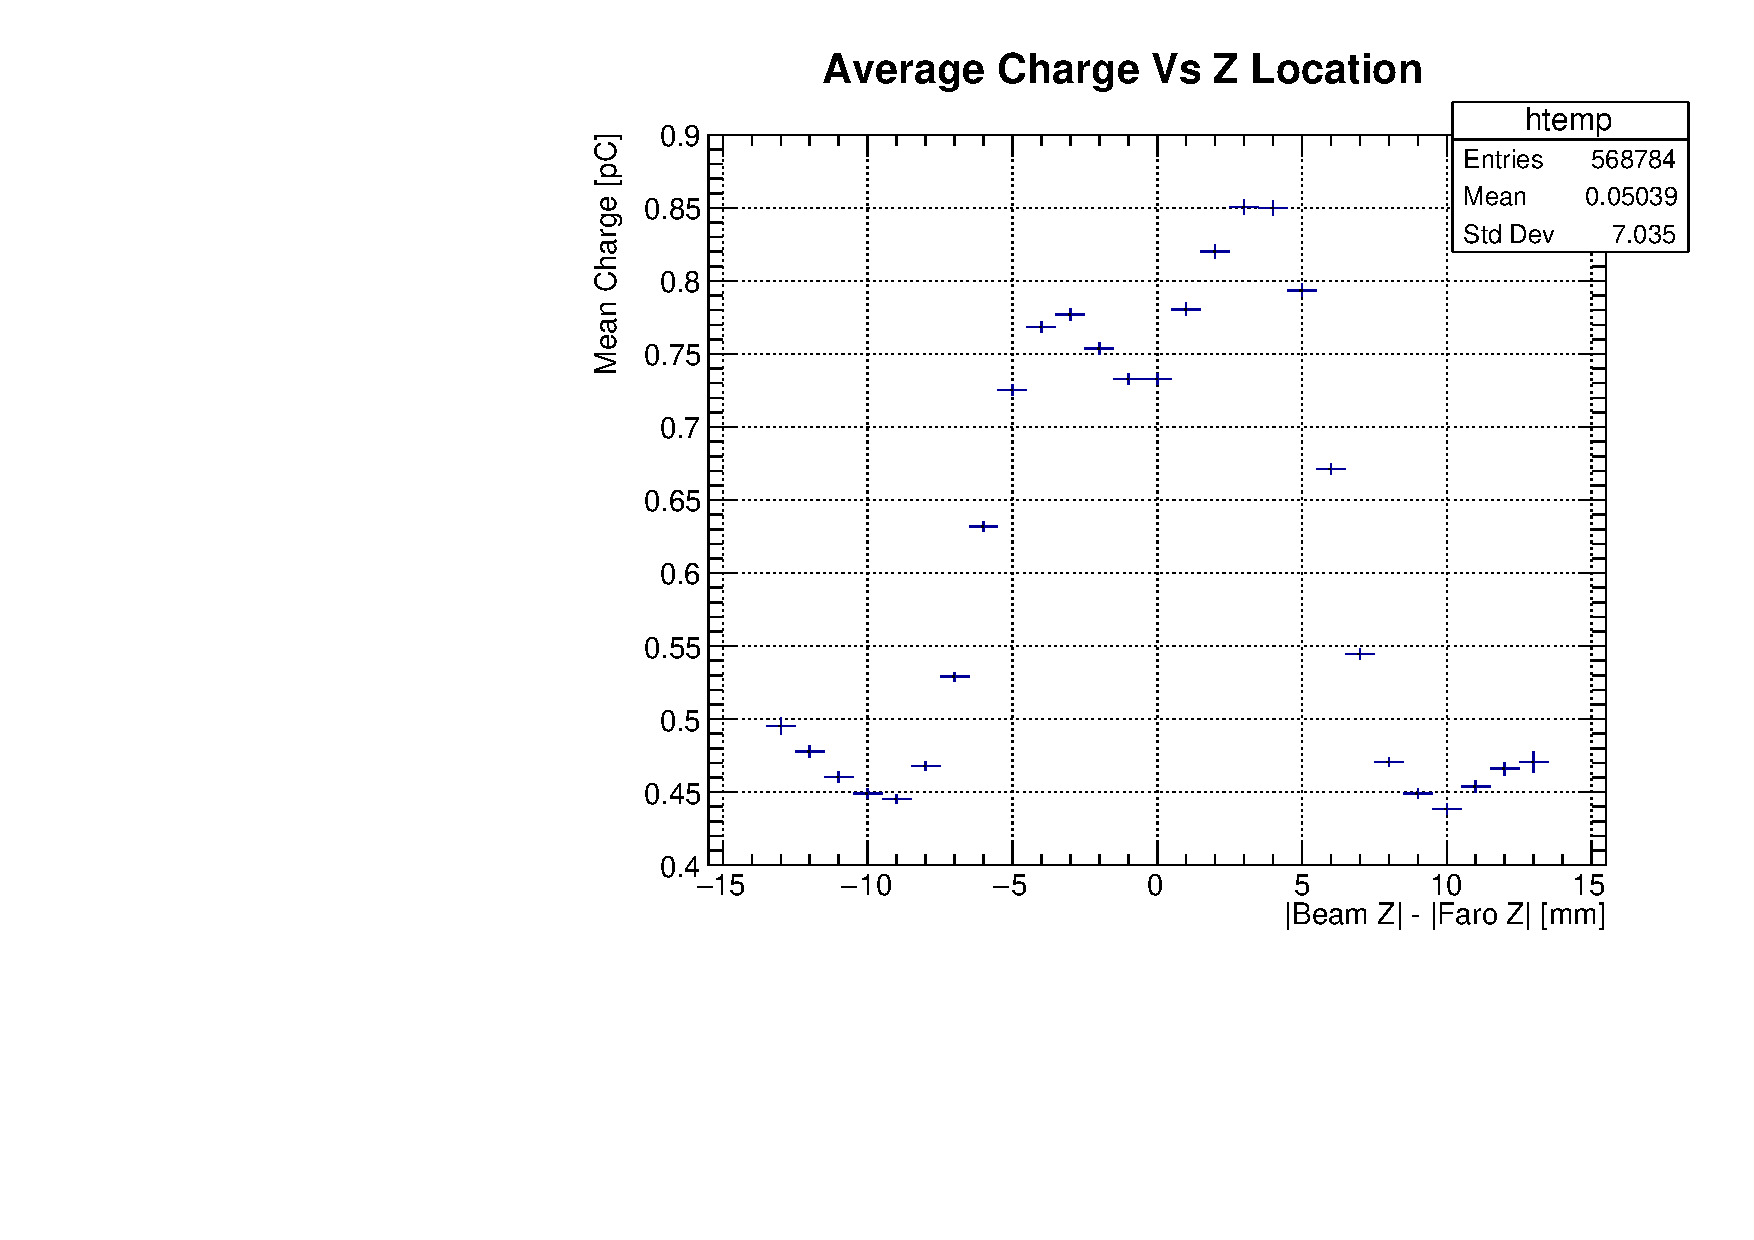
\includegraphics[width=.4\linewidth]{plots/2018/ChargevsZ2}
  \caption{Mean waveform amplitude (left) and charge (left) as a function of X-ray Z coordinate centered
    at nominal photodetector center. Only downstream photodetectors ($Z>0$ mm) are included in the plot.}
  \label{fig:mppcleftright}
\end{figure}

\begin{figure}[h]
    \centering
    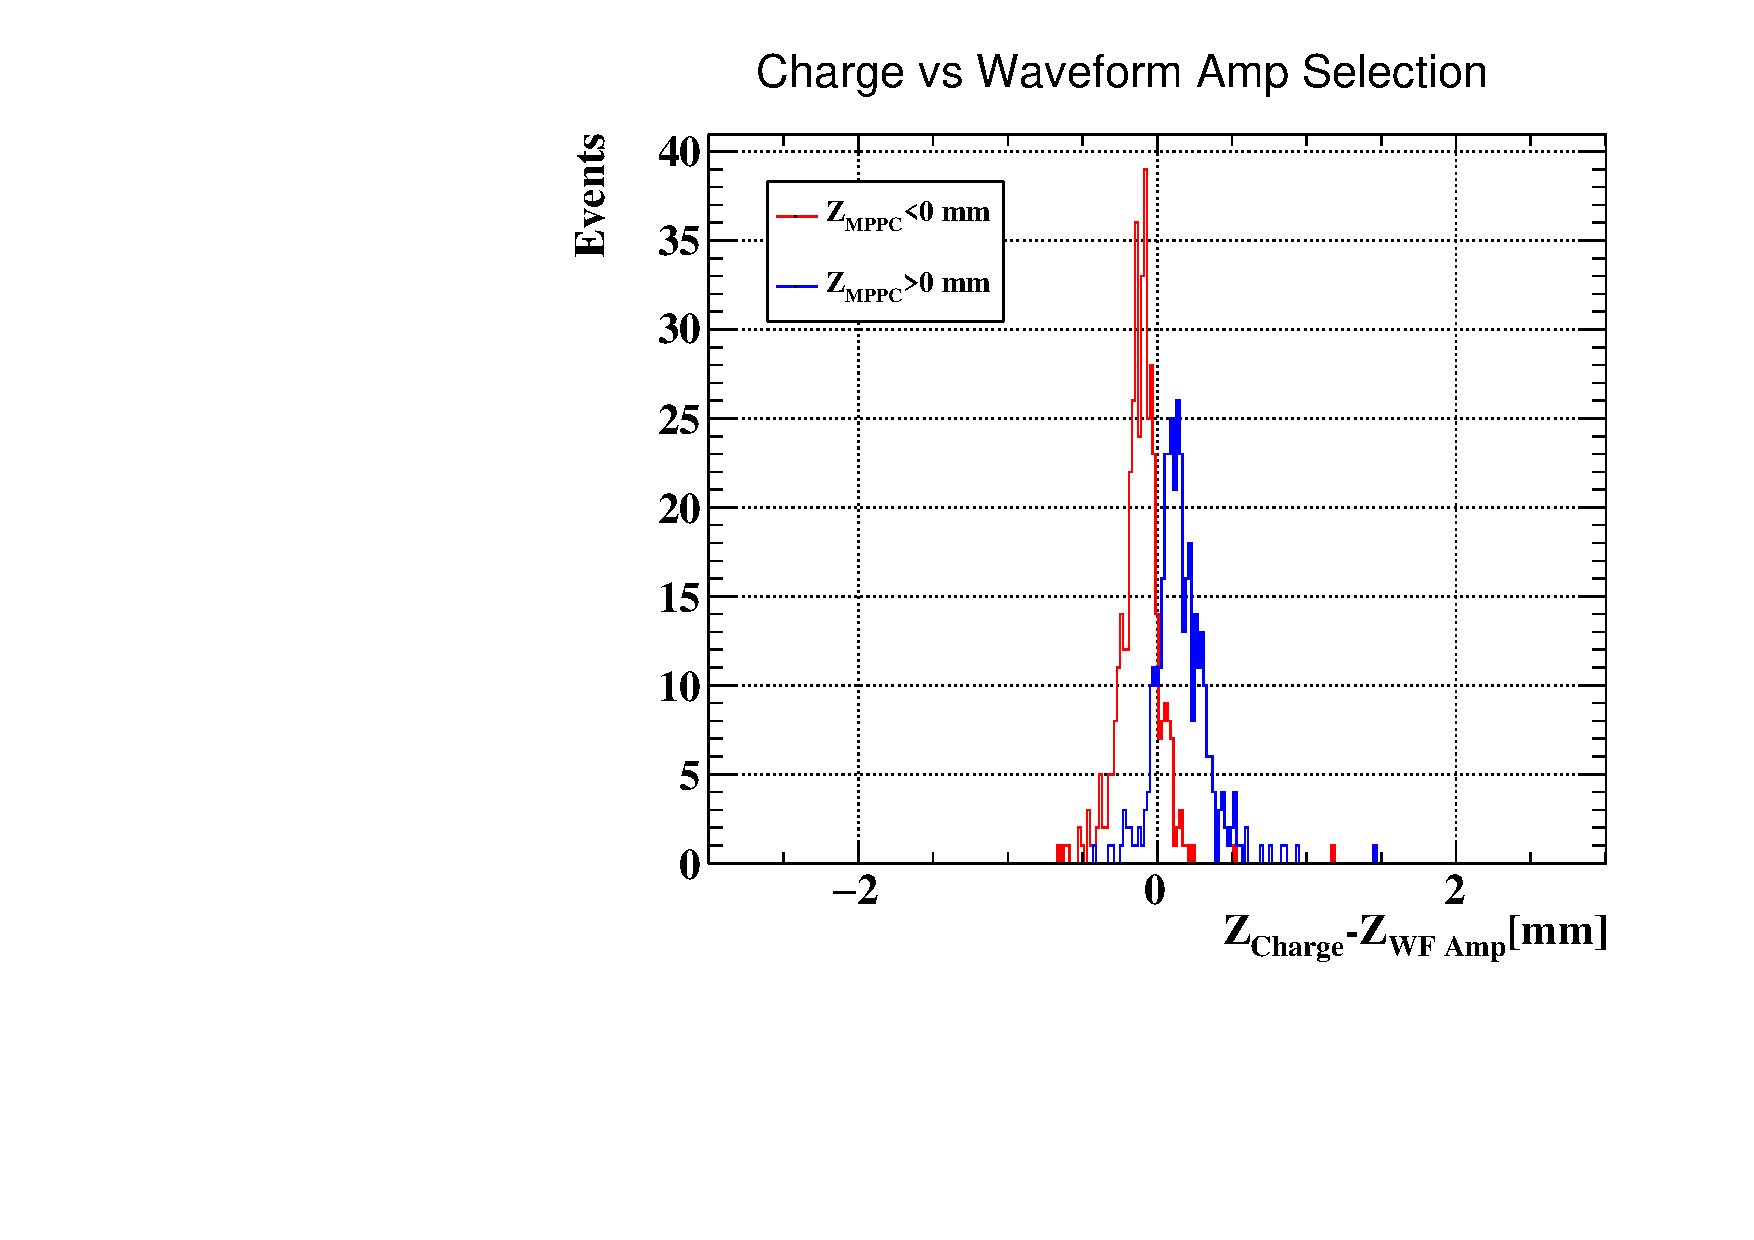
\includegraphics[width=.4\linewidth]{plots/2018/chargevswfampZ}
  \caption{Difference in the reconstructed Z position of the photodetectors 
   due to selection based on charge and waveform amplitude.}
  \label{fig:chargevswfamp}
\end{figure}



\section{Fit Values and Errors}
Fitted parameter values and parameter errors for the primary fit 
function. 

\begin{enumerate}
    \item Z Position Fit Error $<$ 0.3 mm
    \item $\phi$ Position Fit Error $<$ 0.03 deg
    \item Reduced $\chi ^{2} \; <$ 100
\end{enumerate}


\begin{figure}[h]
    \centering
    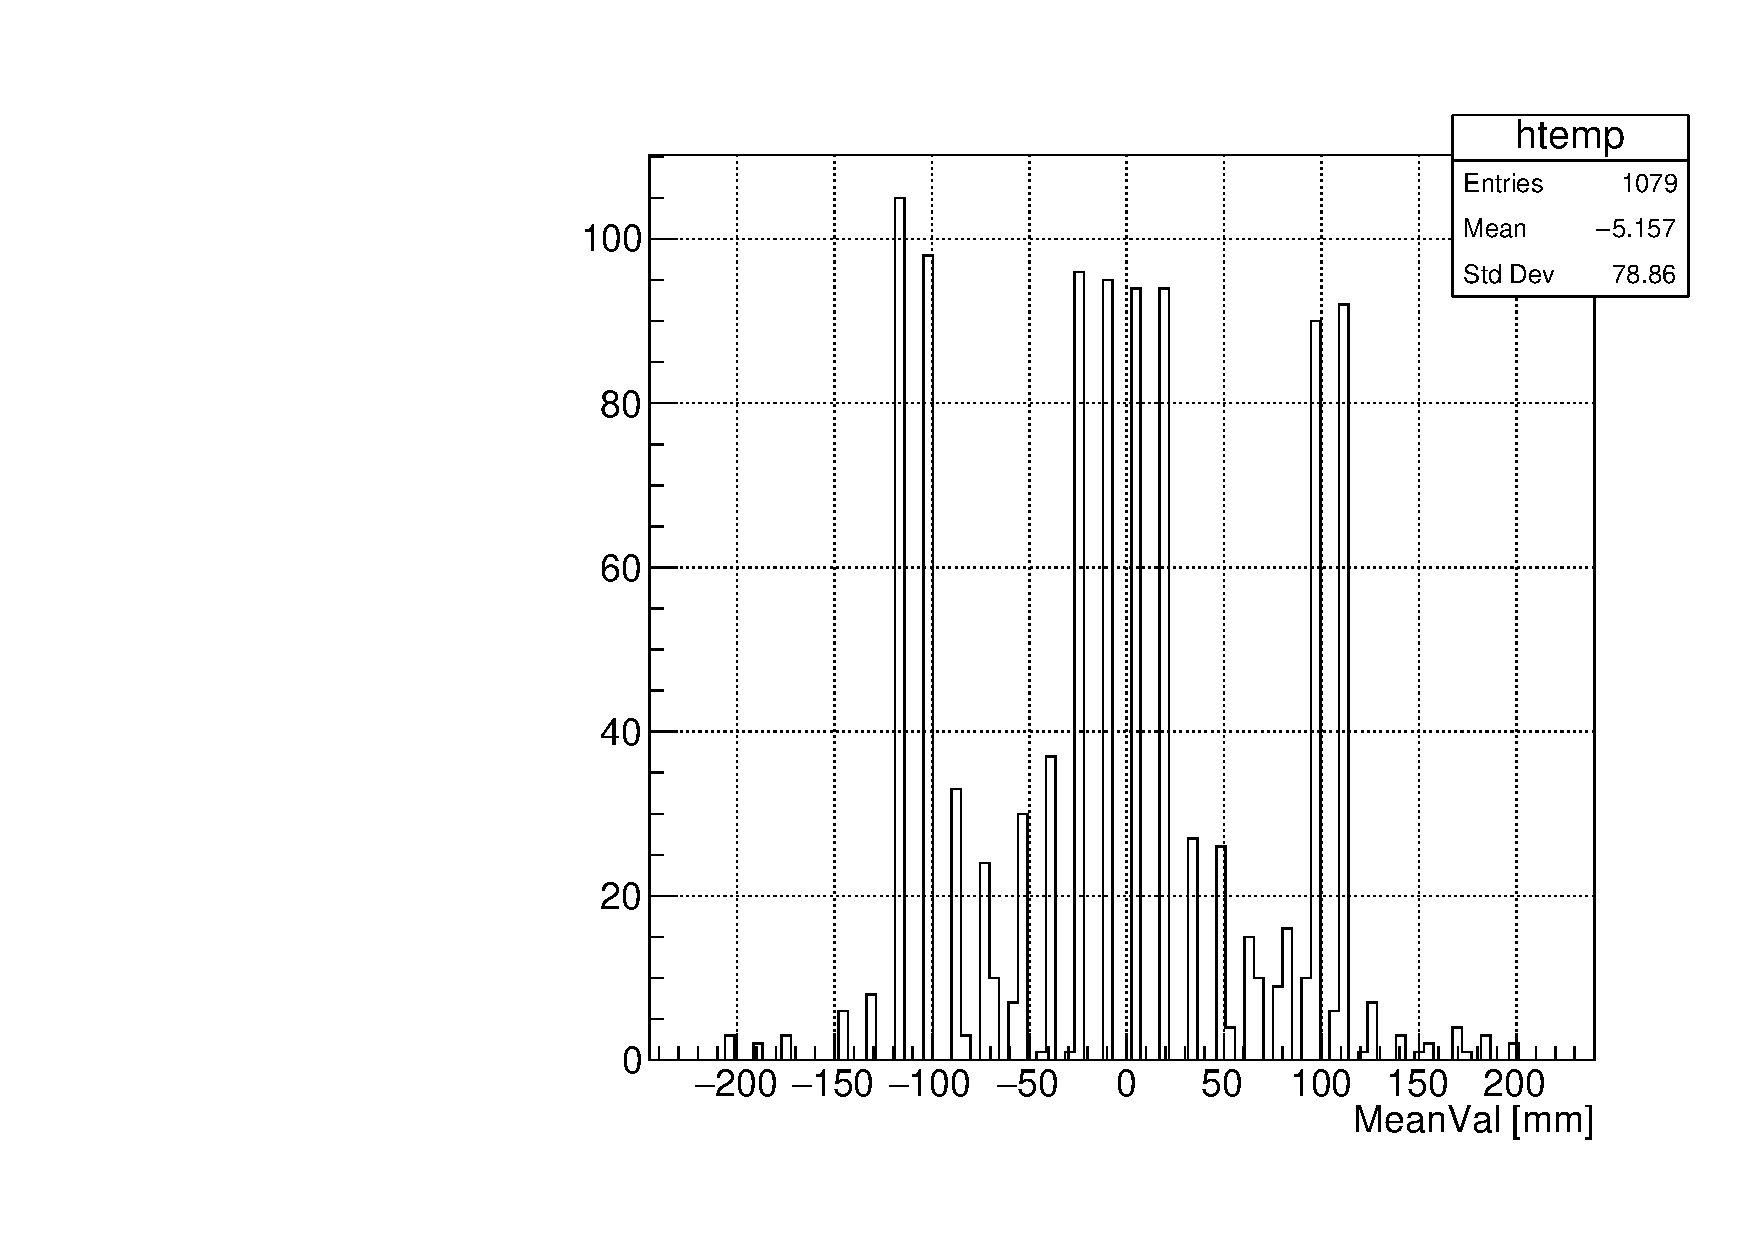
\includegraphics[width=.4\linewidth]{plots/2018/ZMeanVal.pdf}
    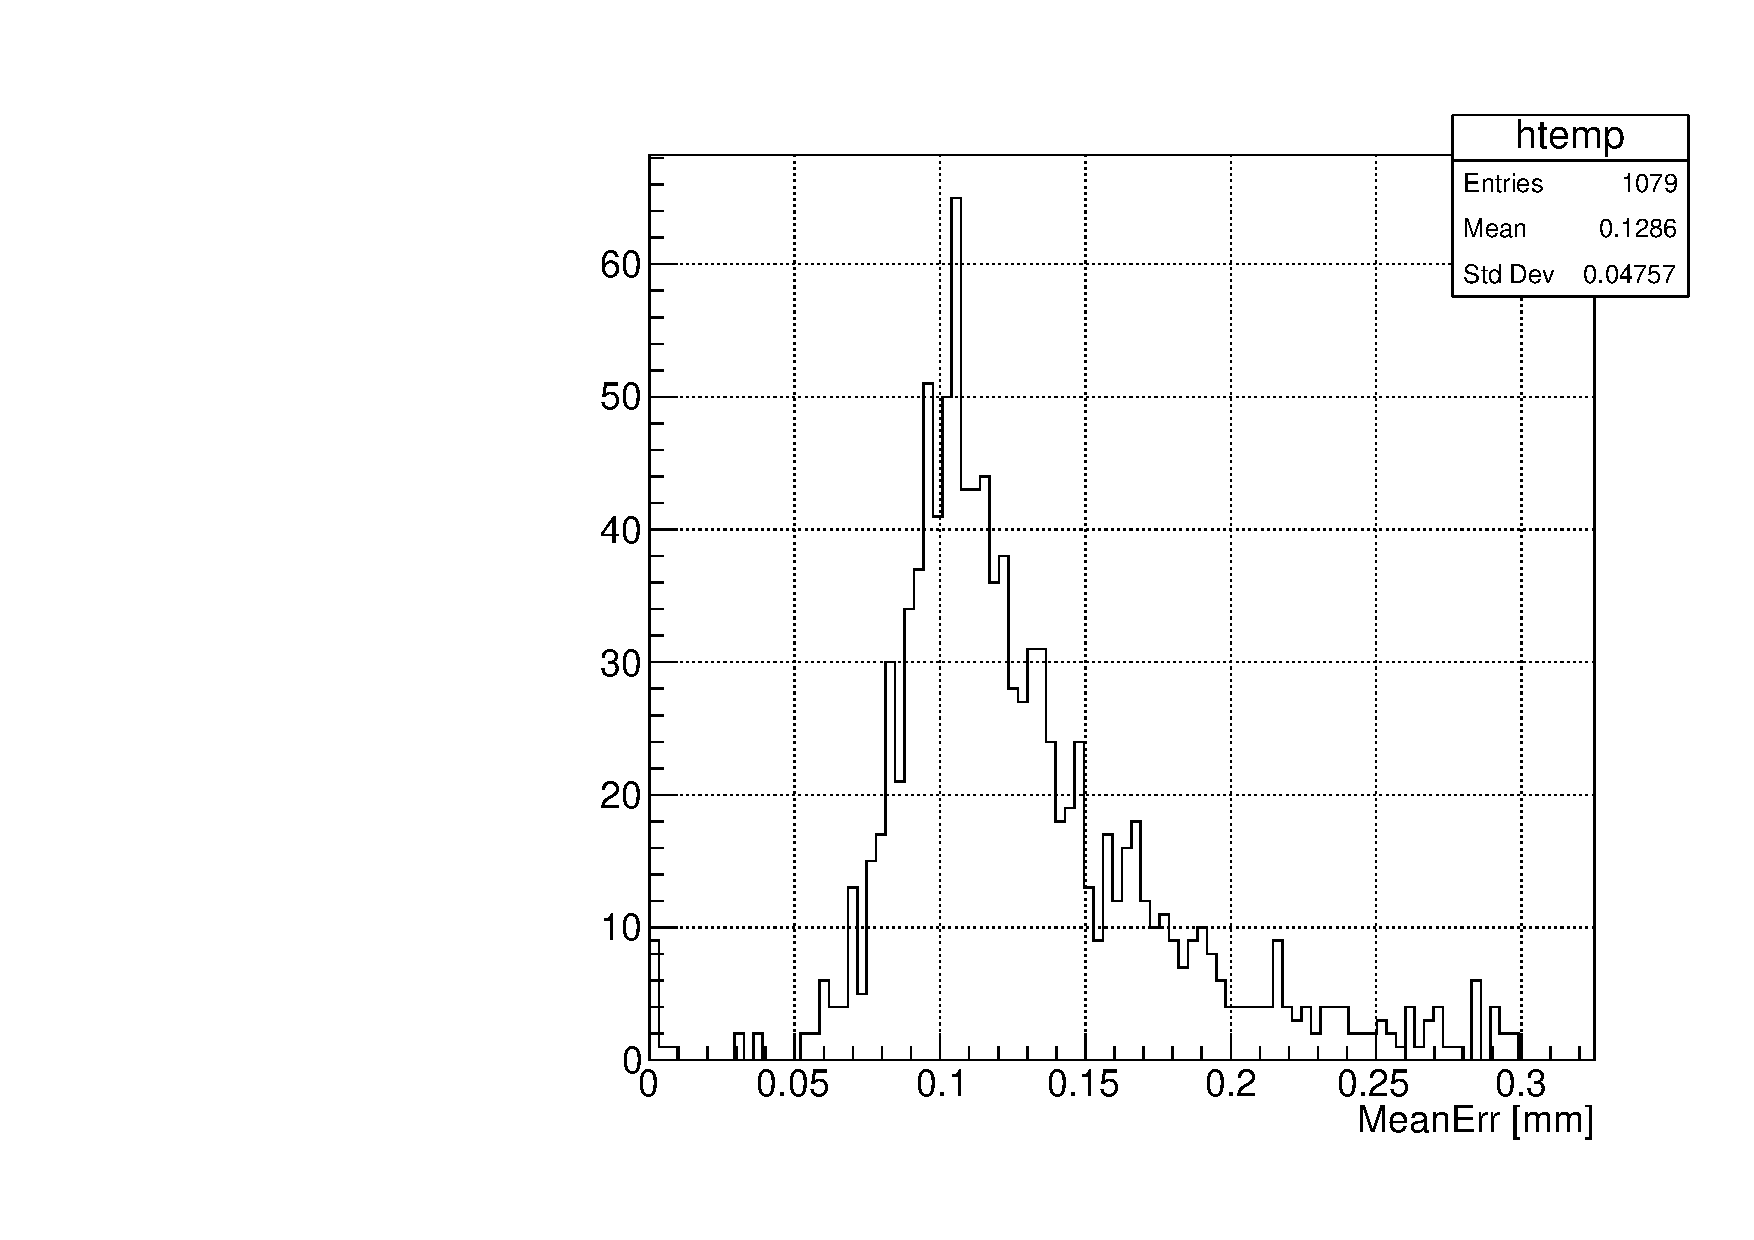
\includegraphics[width=.4\linewidth]{plots/2018/ZMeanErr.pdf}\\
    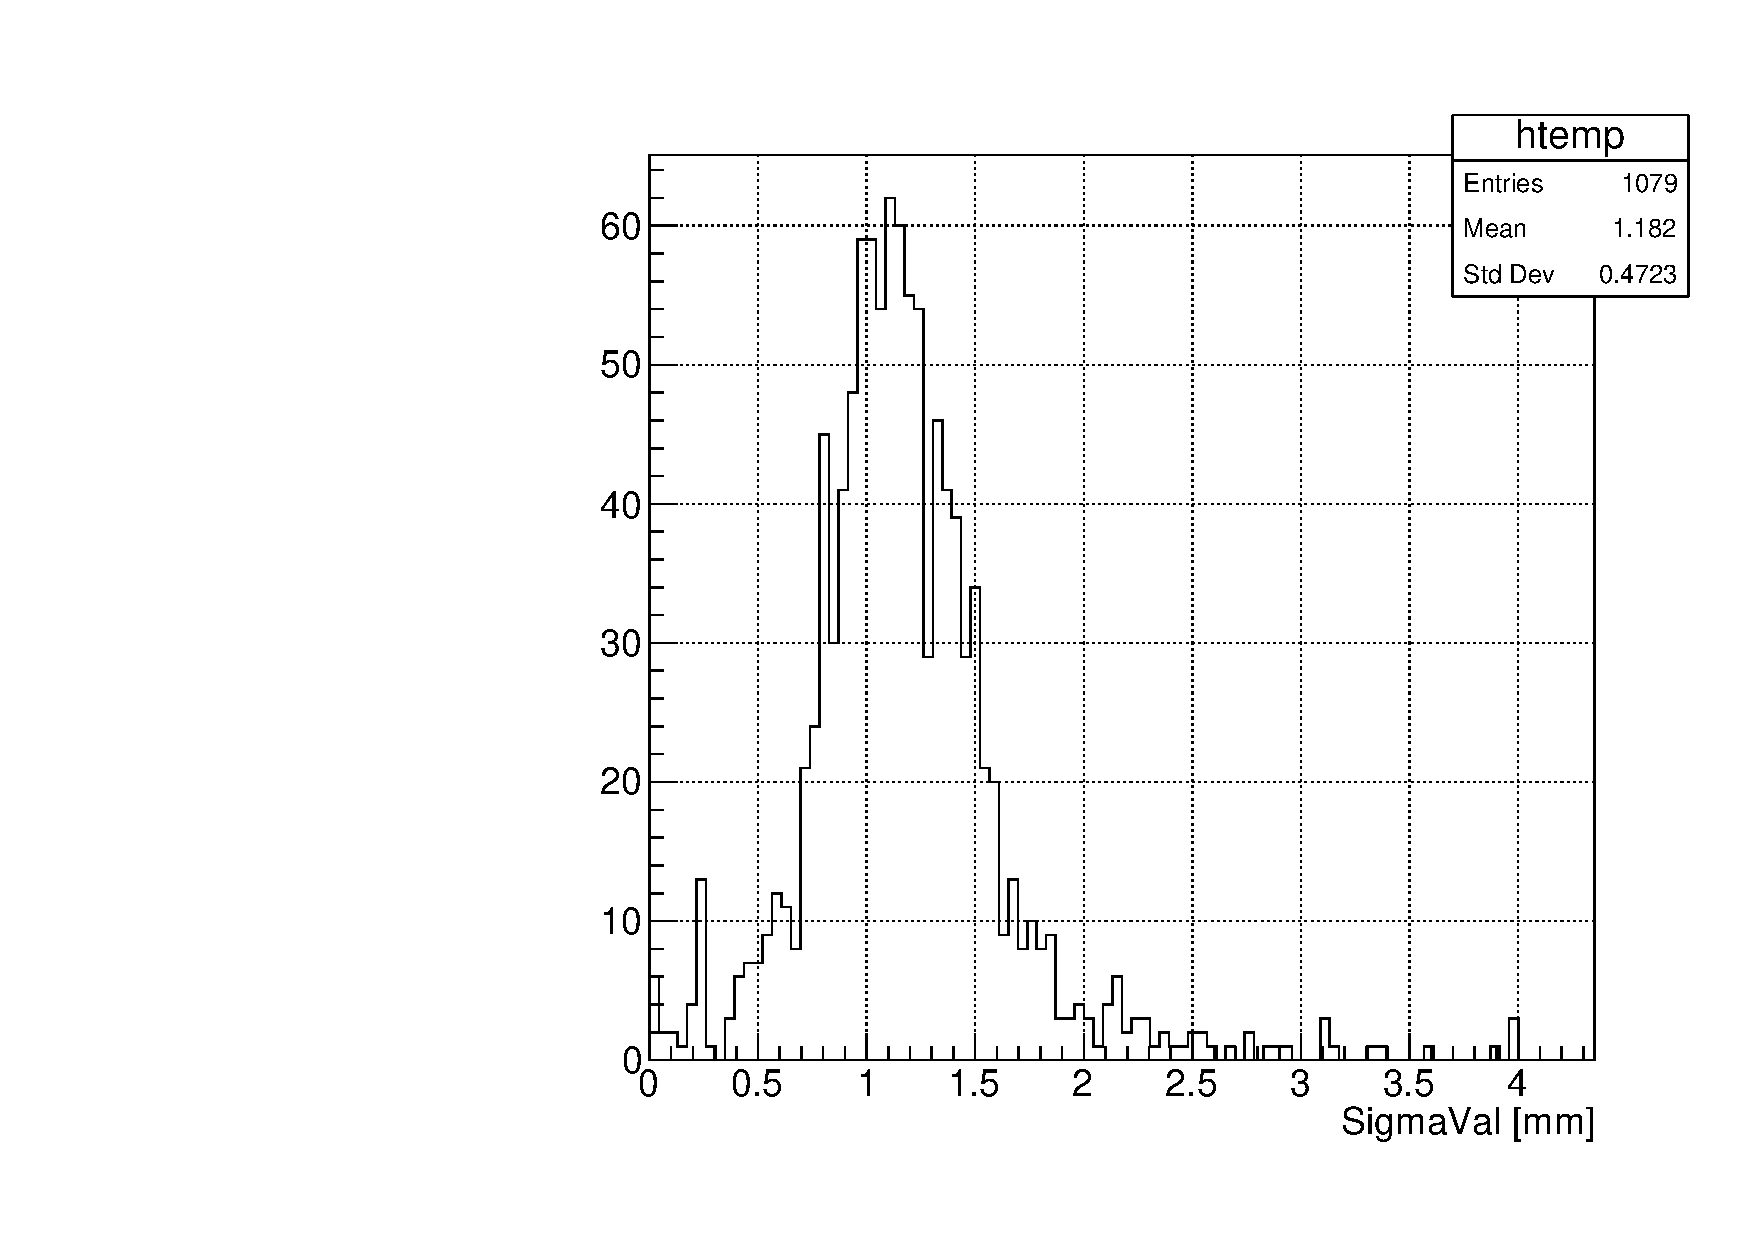
\includegraphics[width=.4\linewidth]{plots/2018/ZSigmaVal.pdf}
    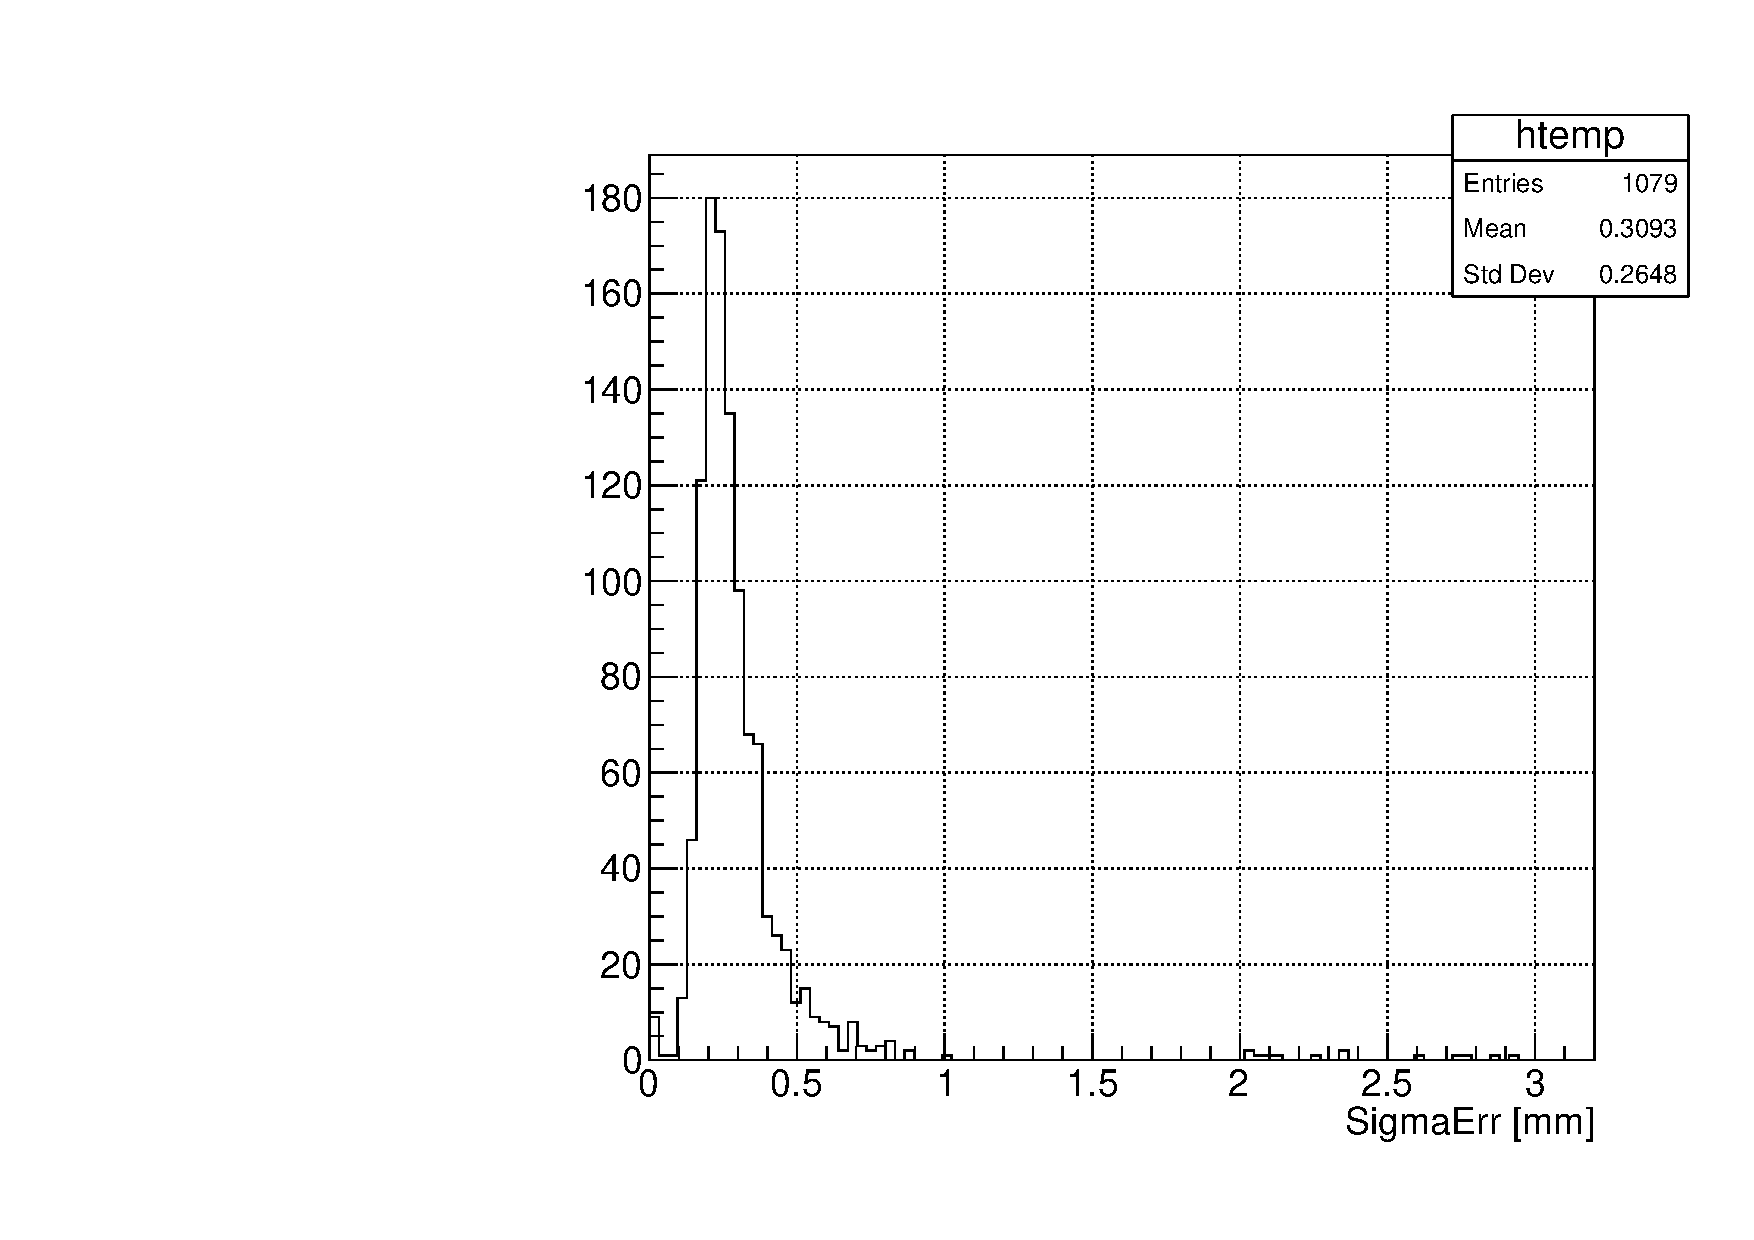
\includegraphics[width=.4\linewidth]{plots/2018/ZSigmaErr.pdf}\\
    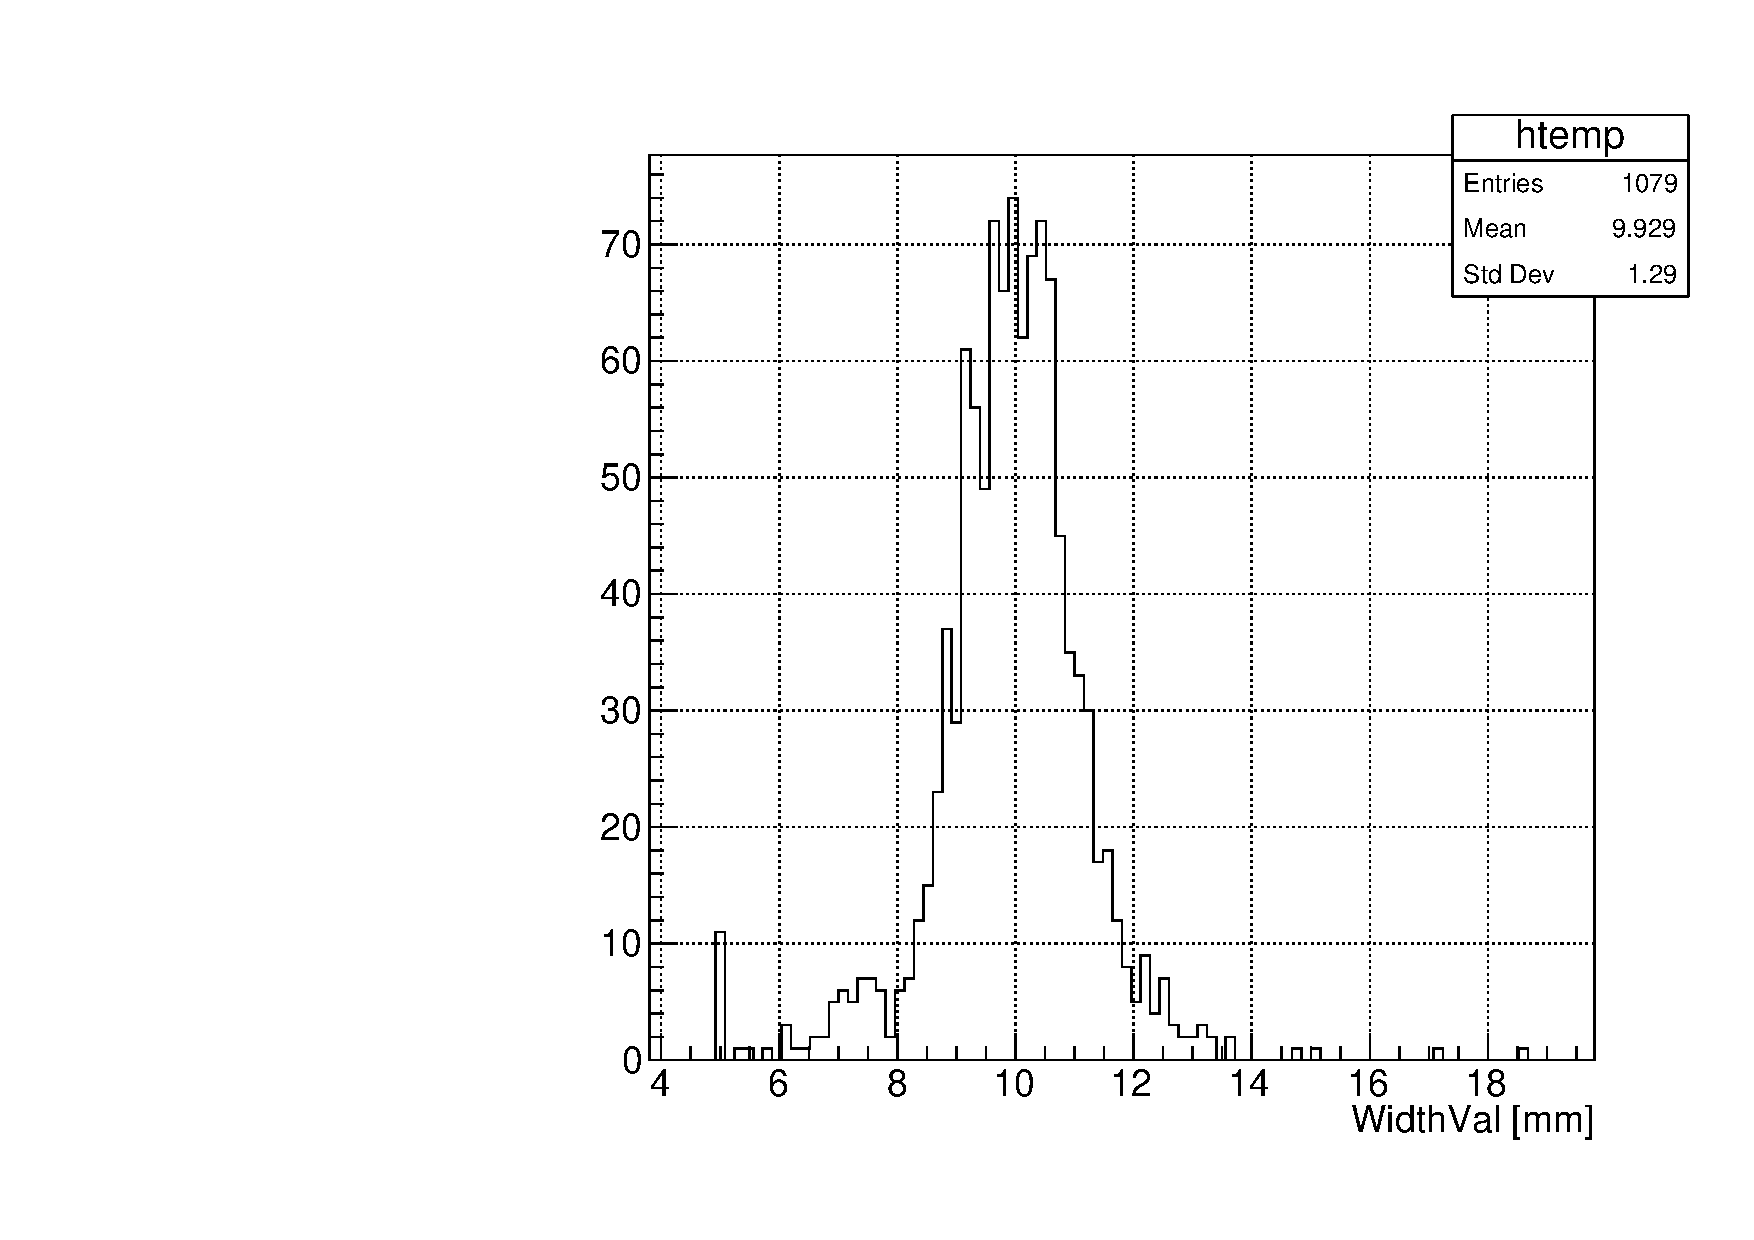
\includegraphics[width=.4\linewidth]{plots/2018/ZWidthVal.pdf}
    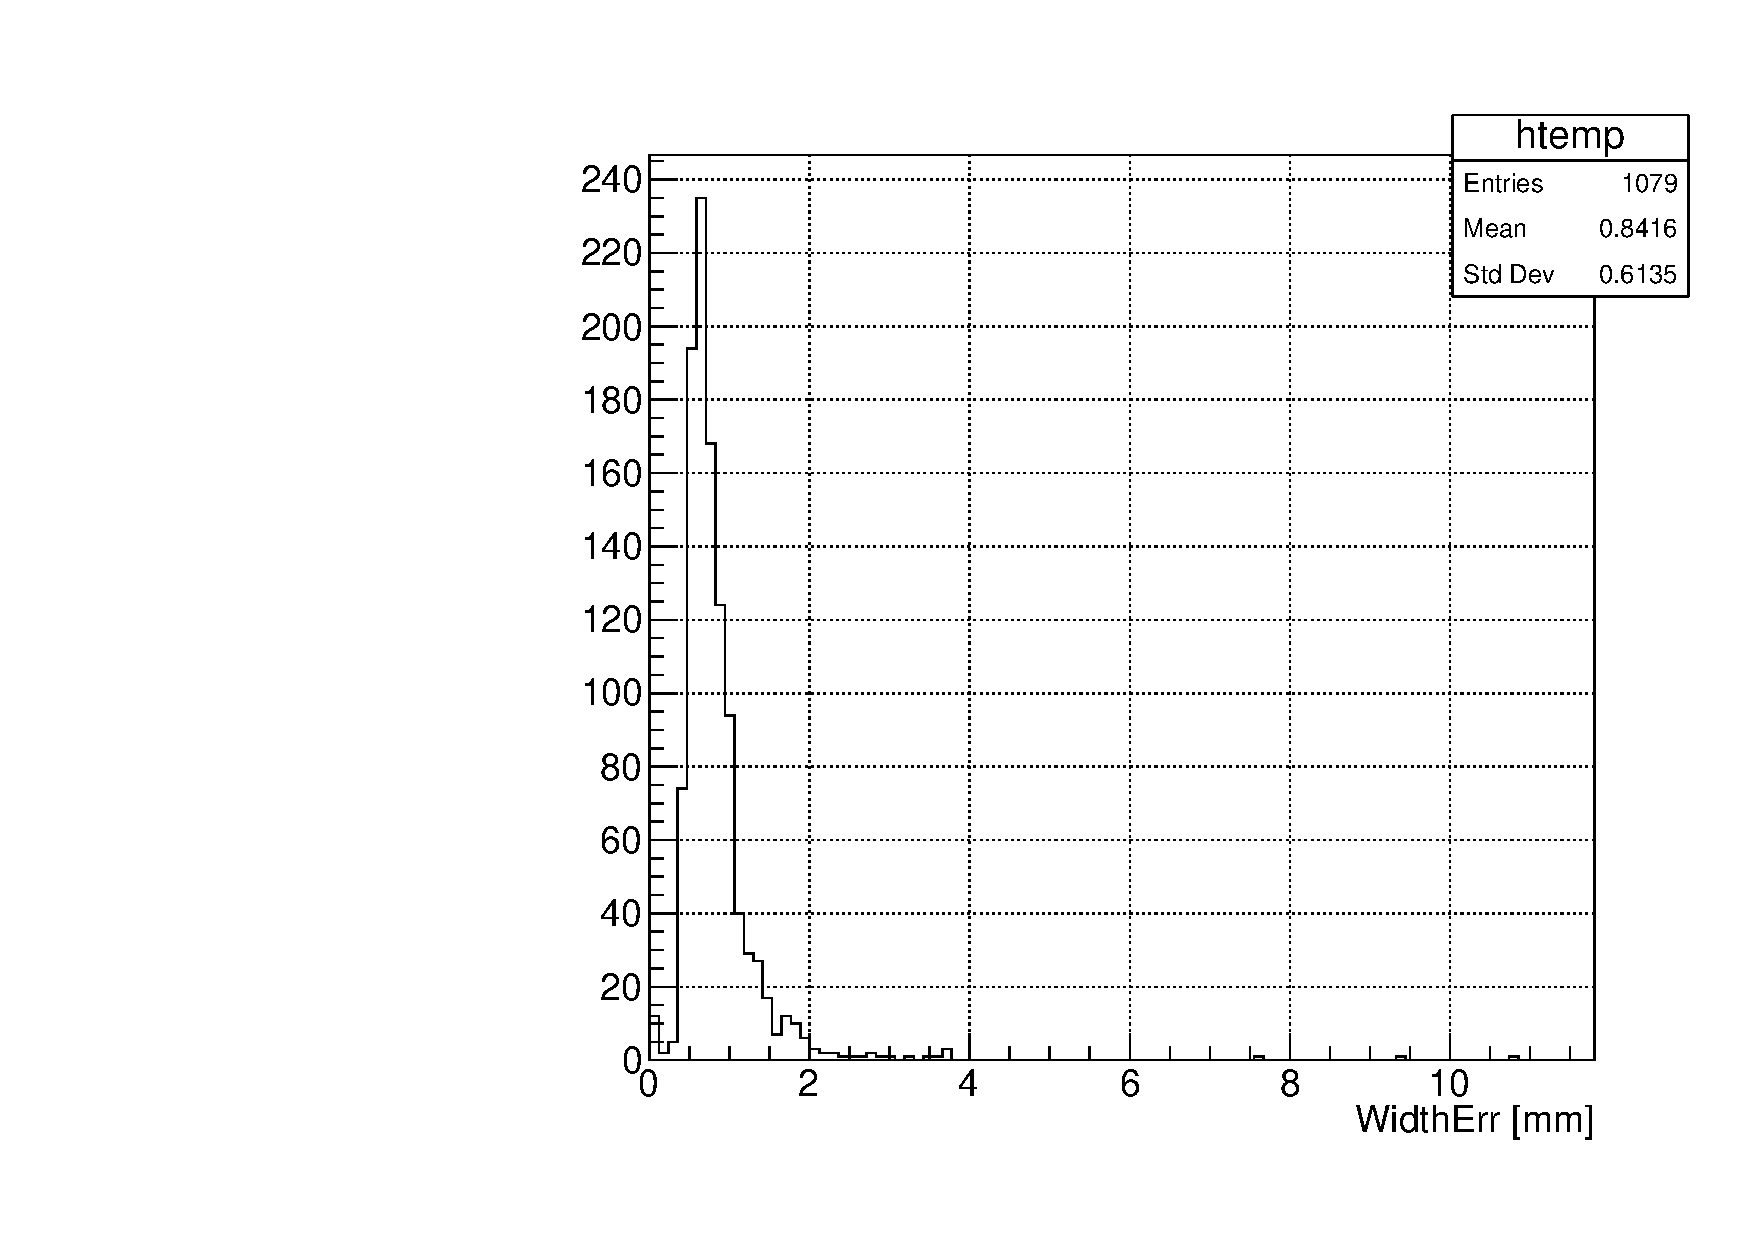
\includegraphics[width=.4\linewidth]{plots/2018/ZWidthErr.pdf}\\
    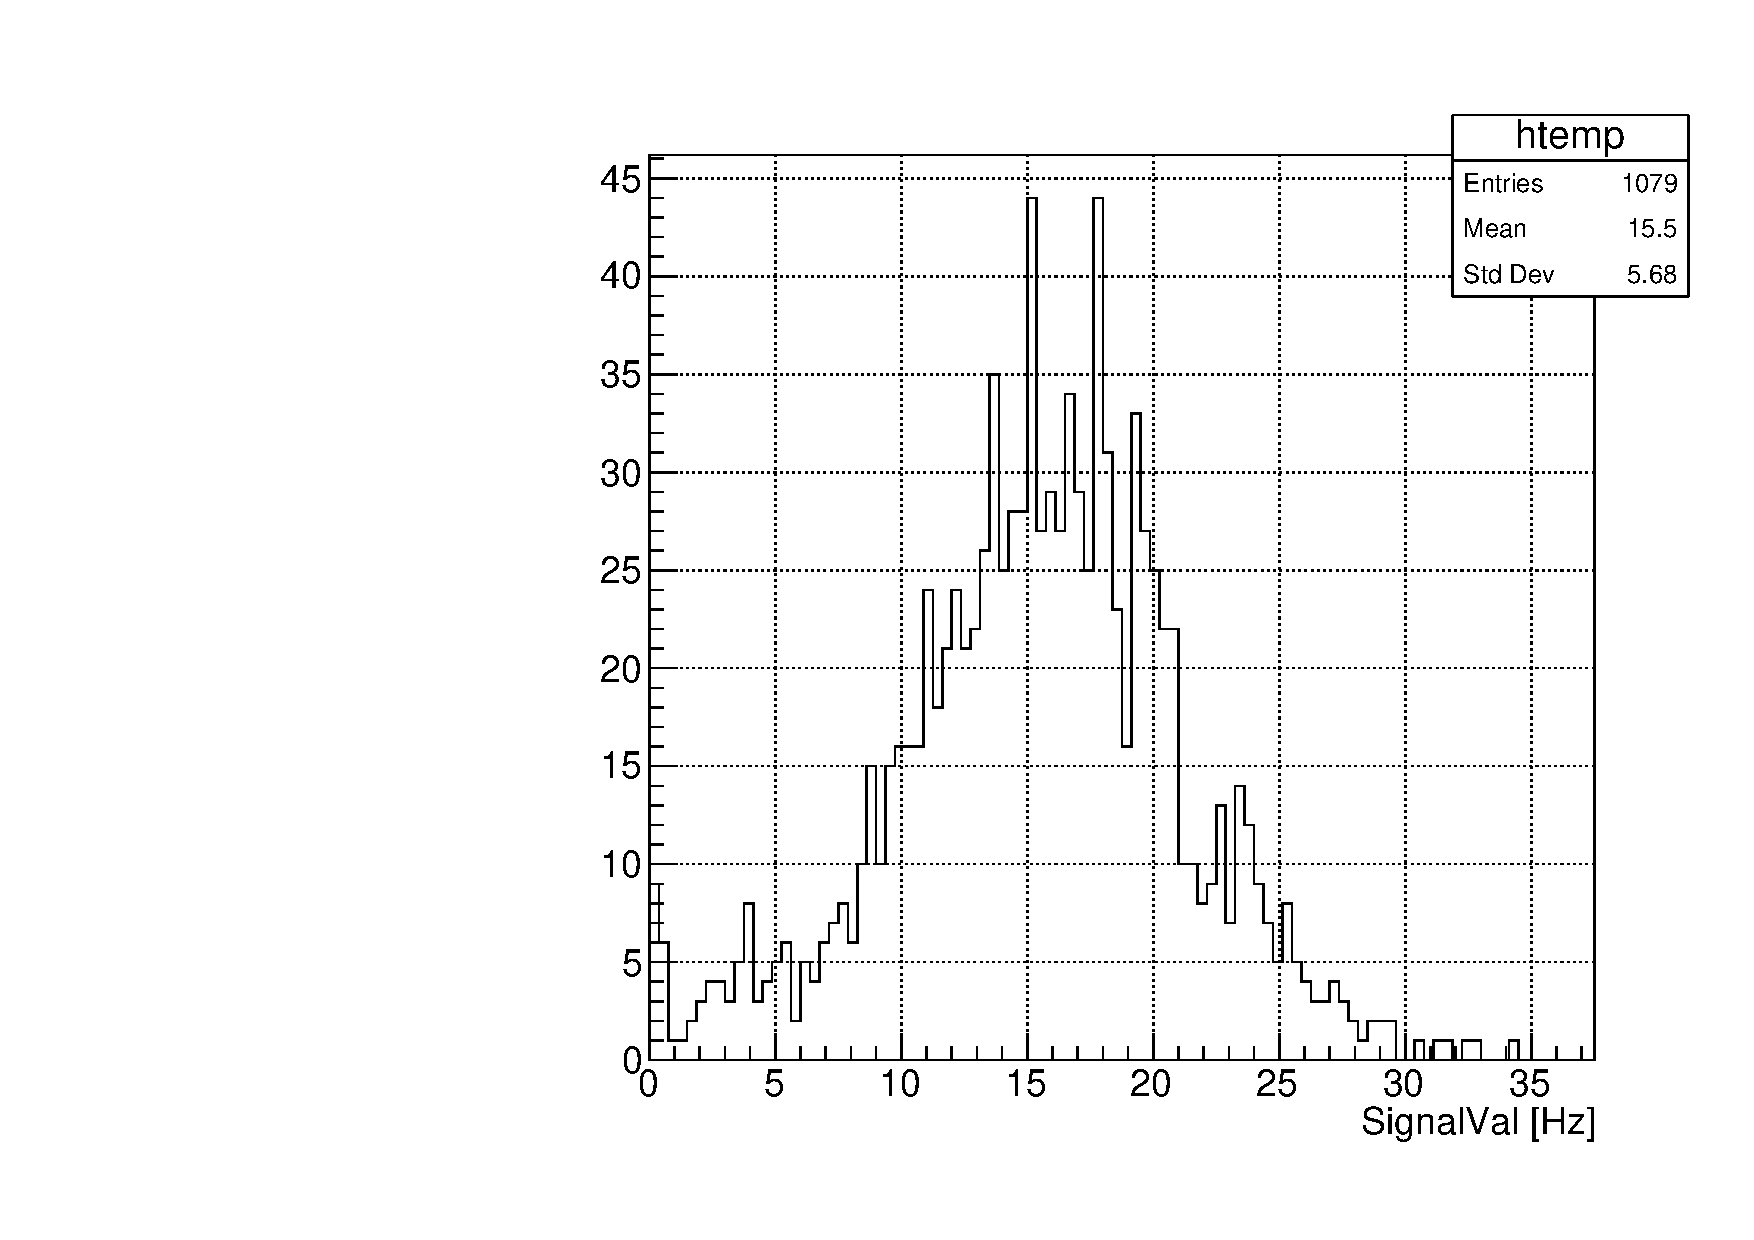
\includegraphics[width=.4\linewidth]{plots/2018/ZSignalVal.pdf}
    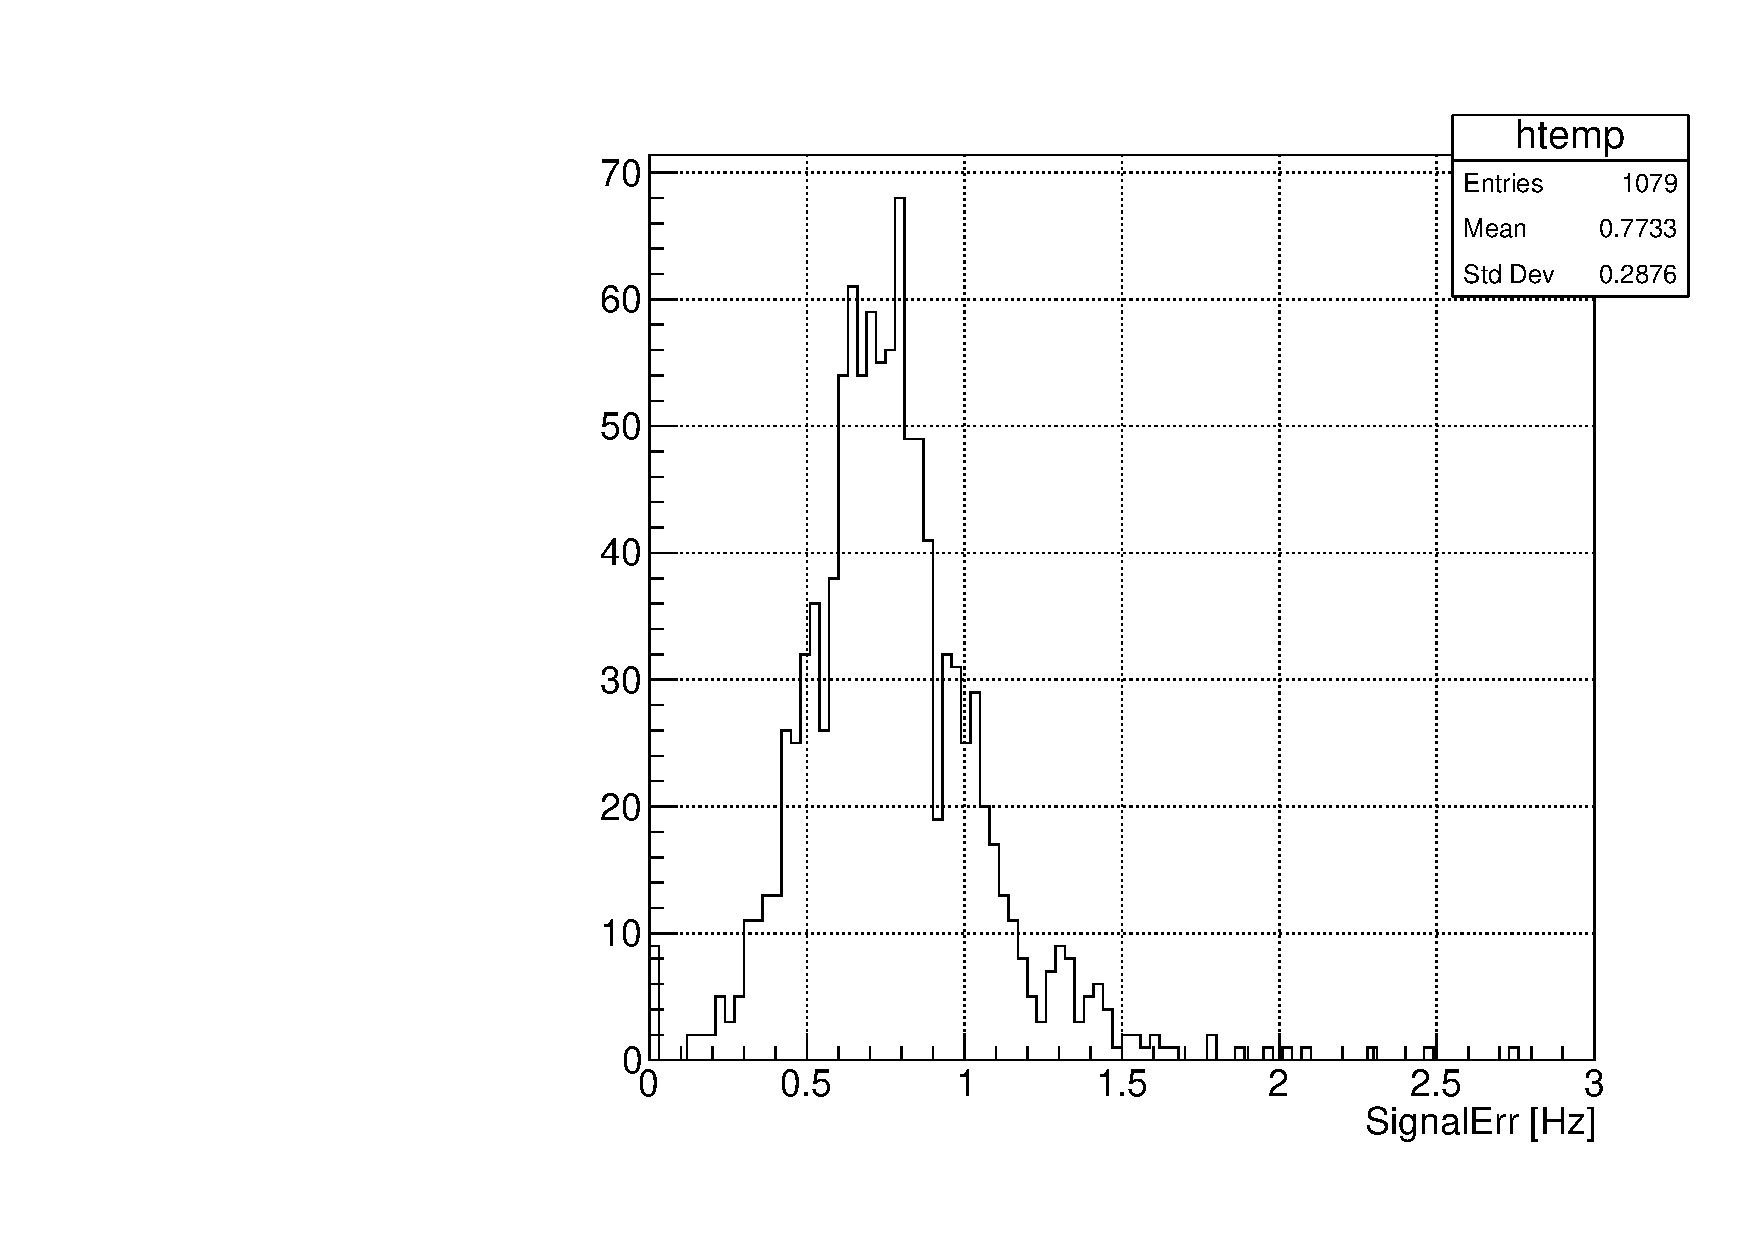
\includegraphics[width=.4\linewidth]{plots/2018/ZSignalErr.pdf}\\
    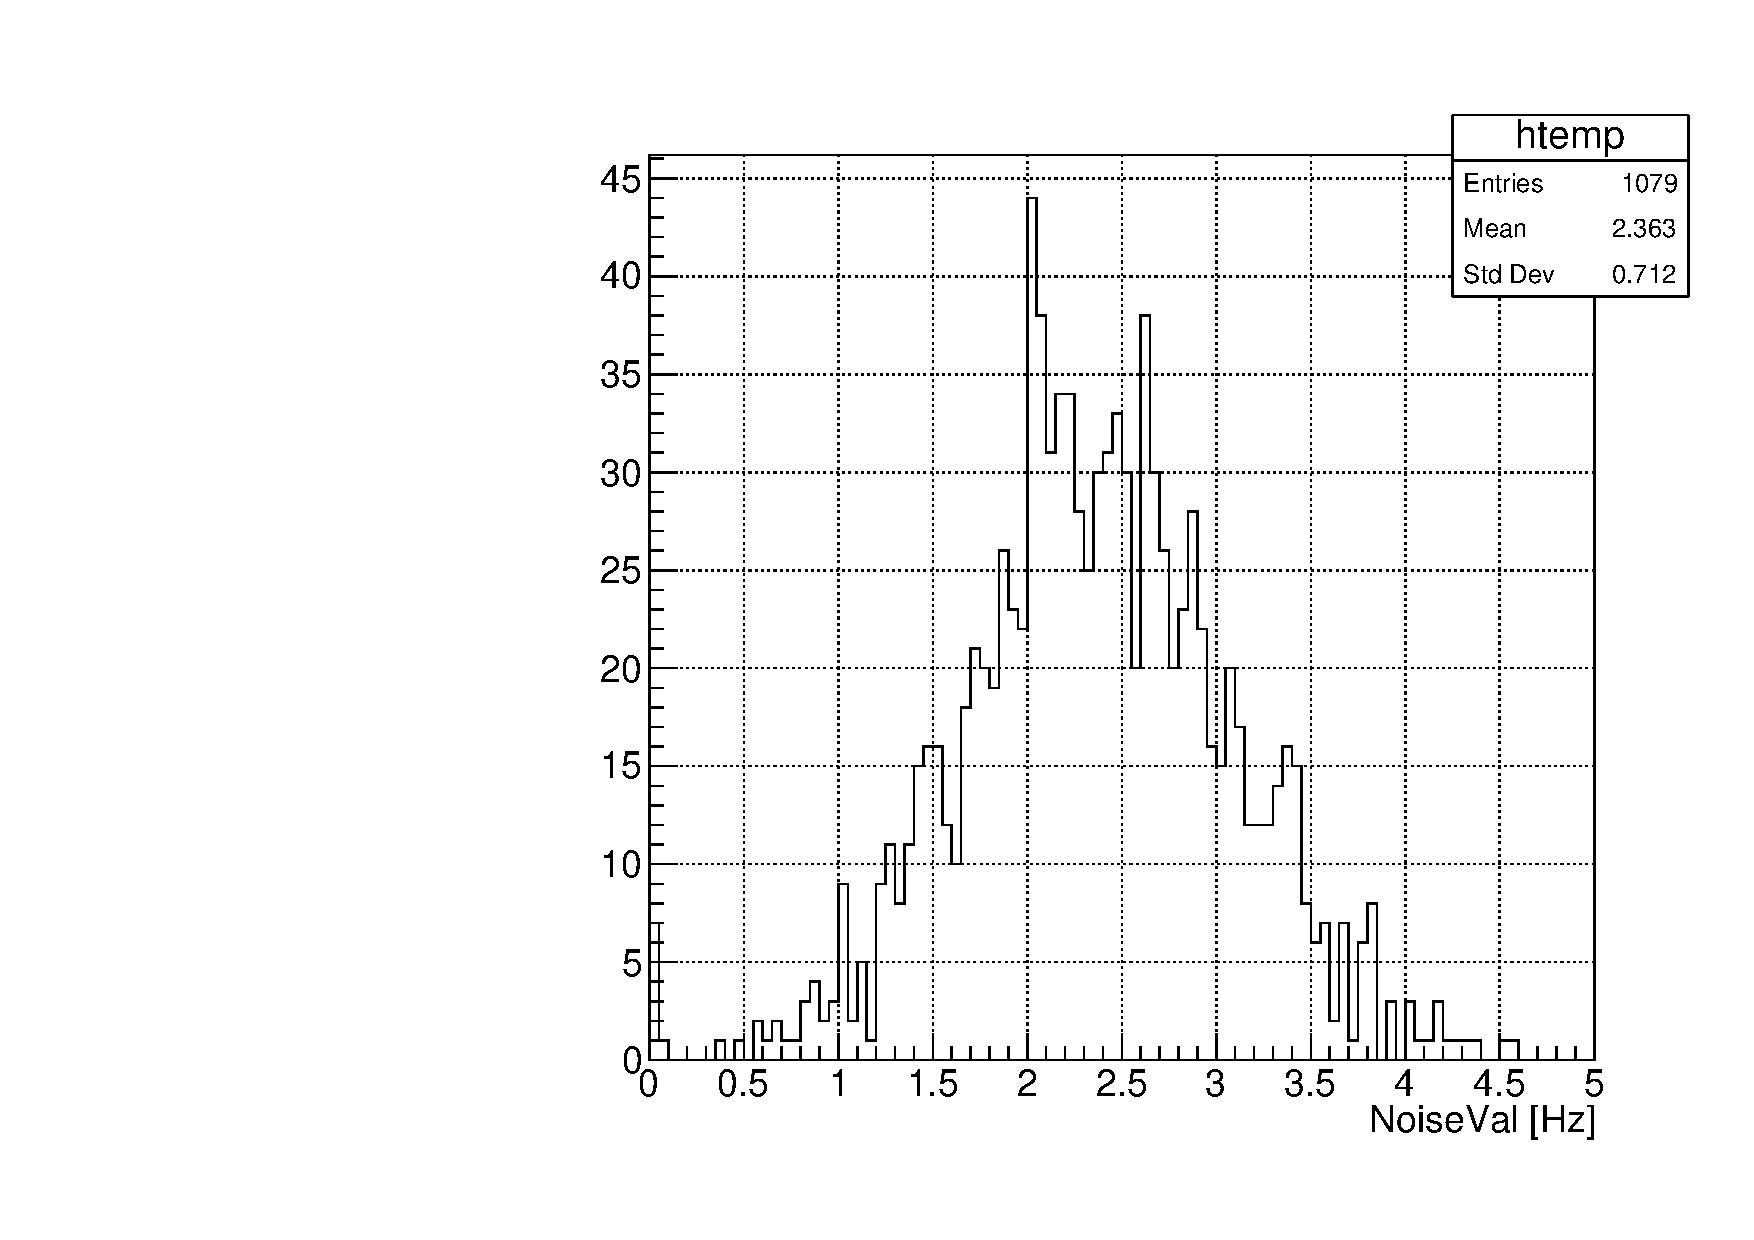
\includegraphics[width=.4\linewidth]{plots/2018/ZNoiseVal.pdf}
    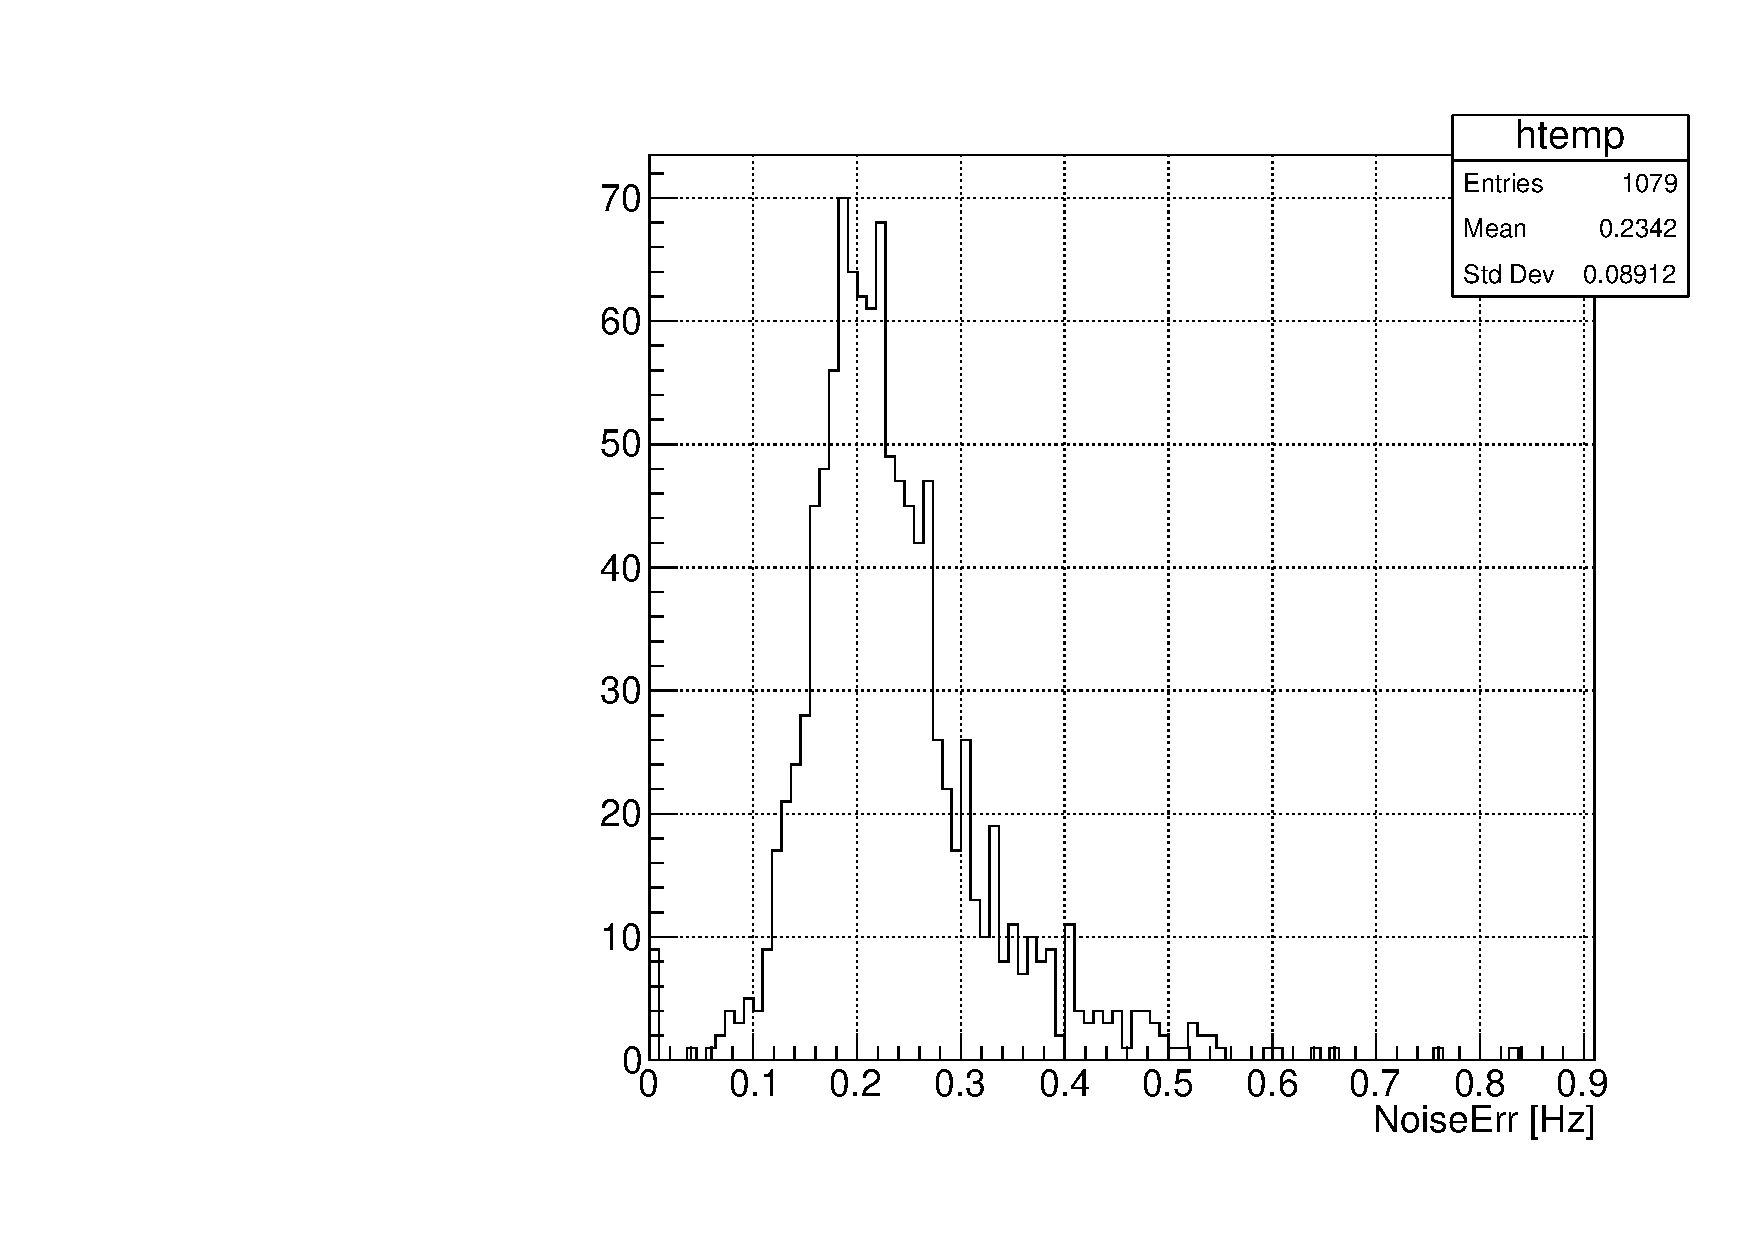
\includegraphics[width=.4\linewidth]{plots/2018/ZNoiseErr.pdf}
    \caption{Fitted parameter values (left) and errors (right) for Z position fits.}
    \label{fig:zfitpars}
\end{figure}

\begin{figure}[h]
    \centering
    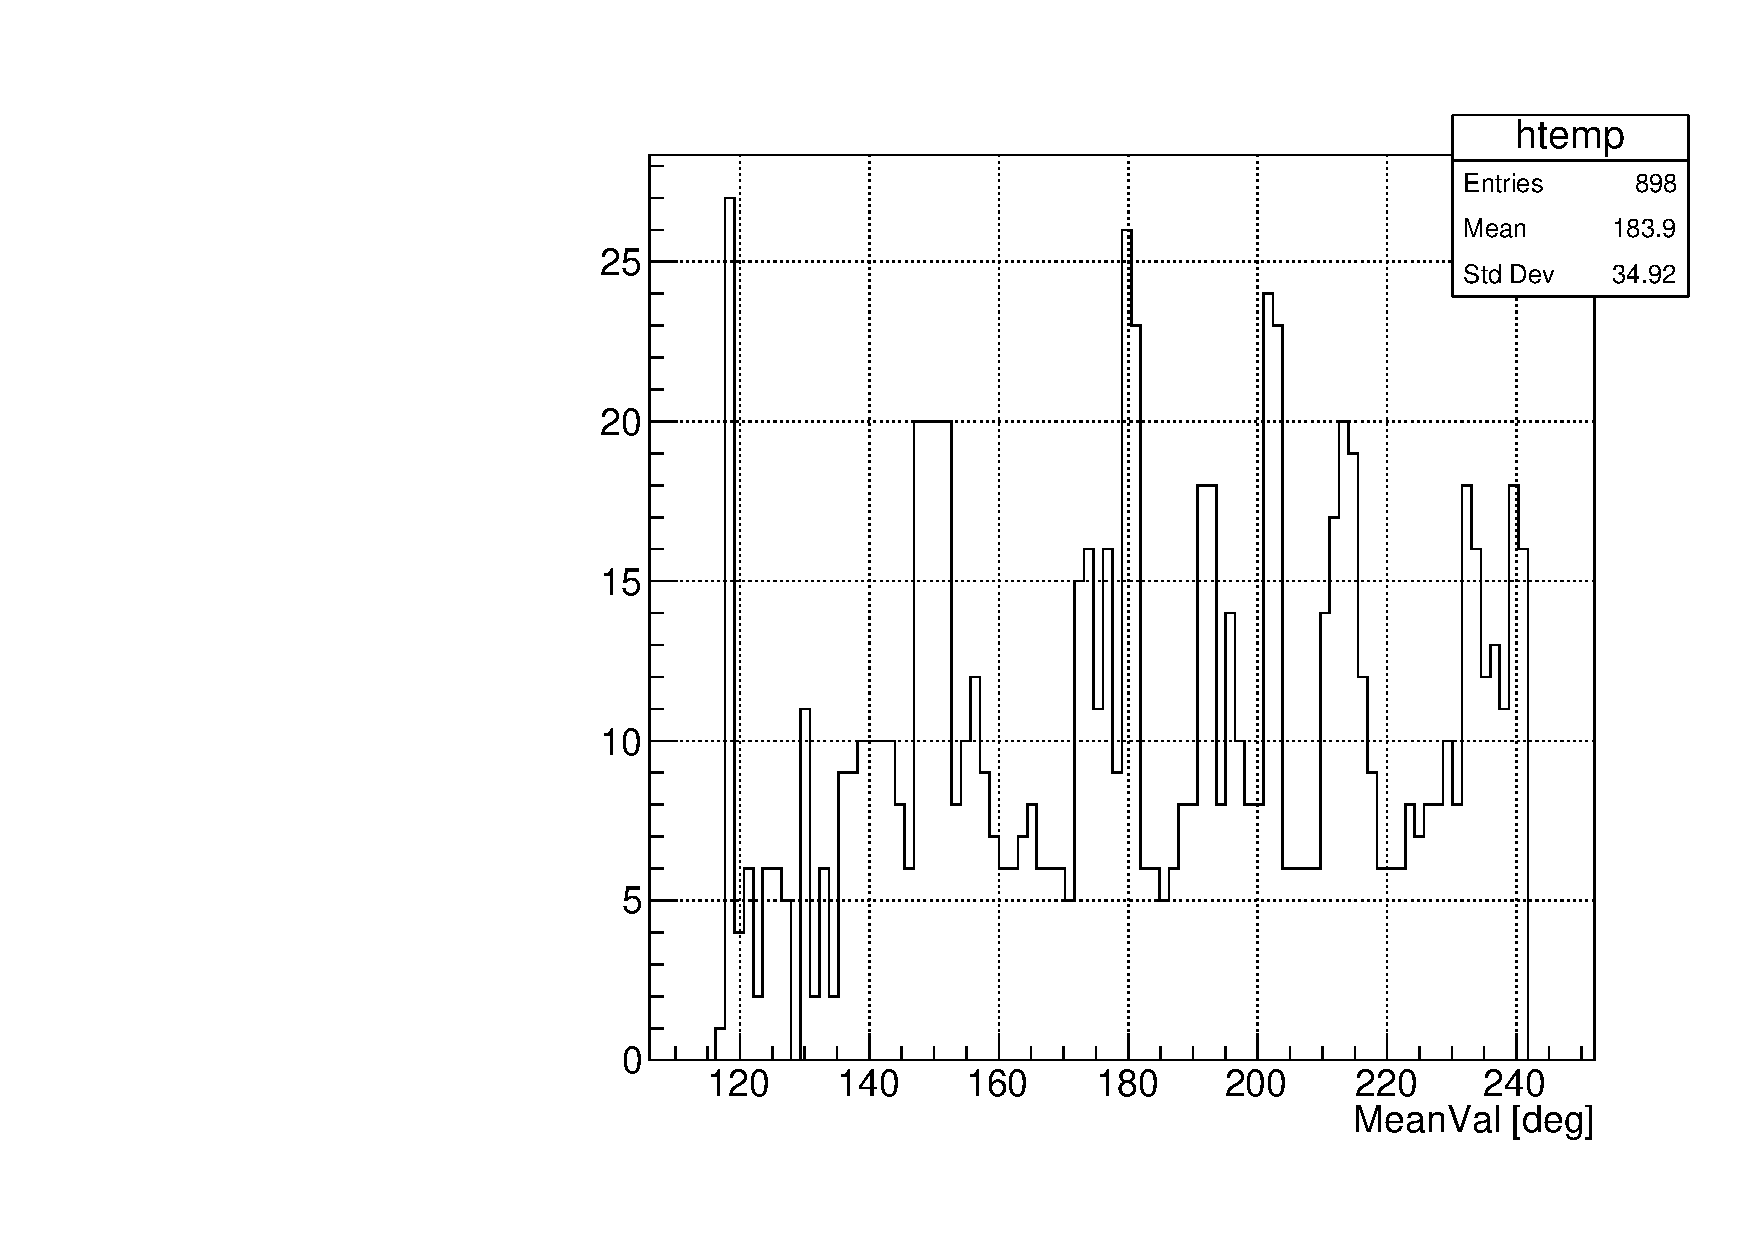
\includegraphics[width=.4\linewidth]{plots/2018/PhiMeanVal.pdf}
    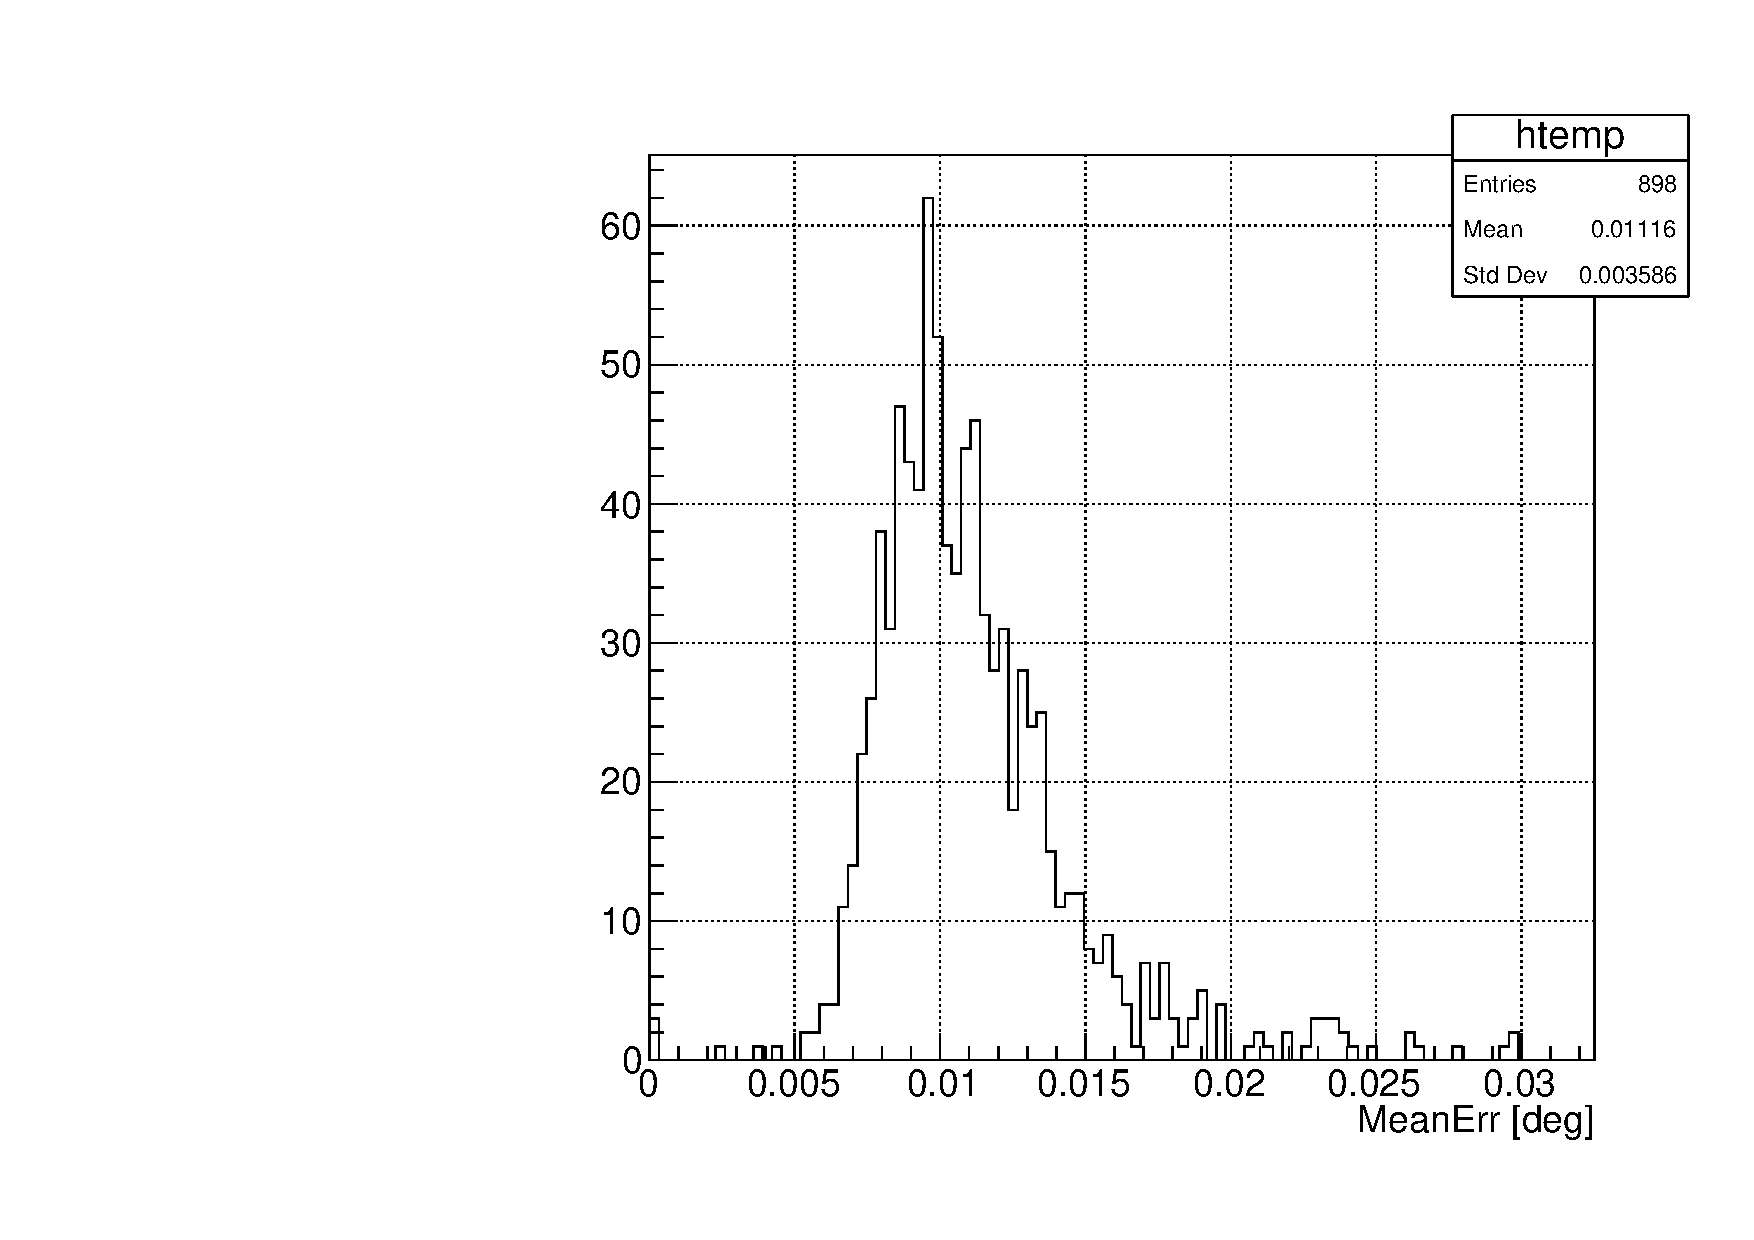
\includegraphics[width=.4\linewidth]{plots/2018/PhiMeanErr.pdf}\\
    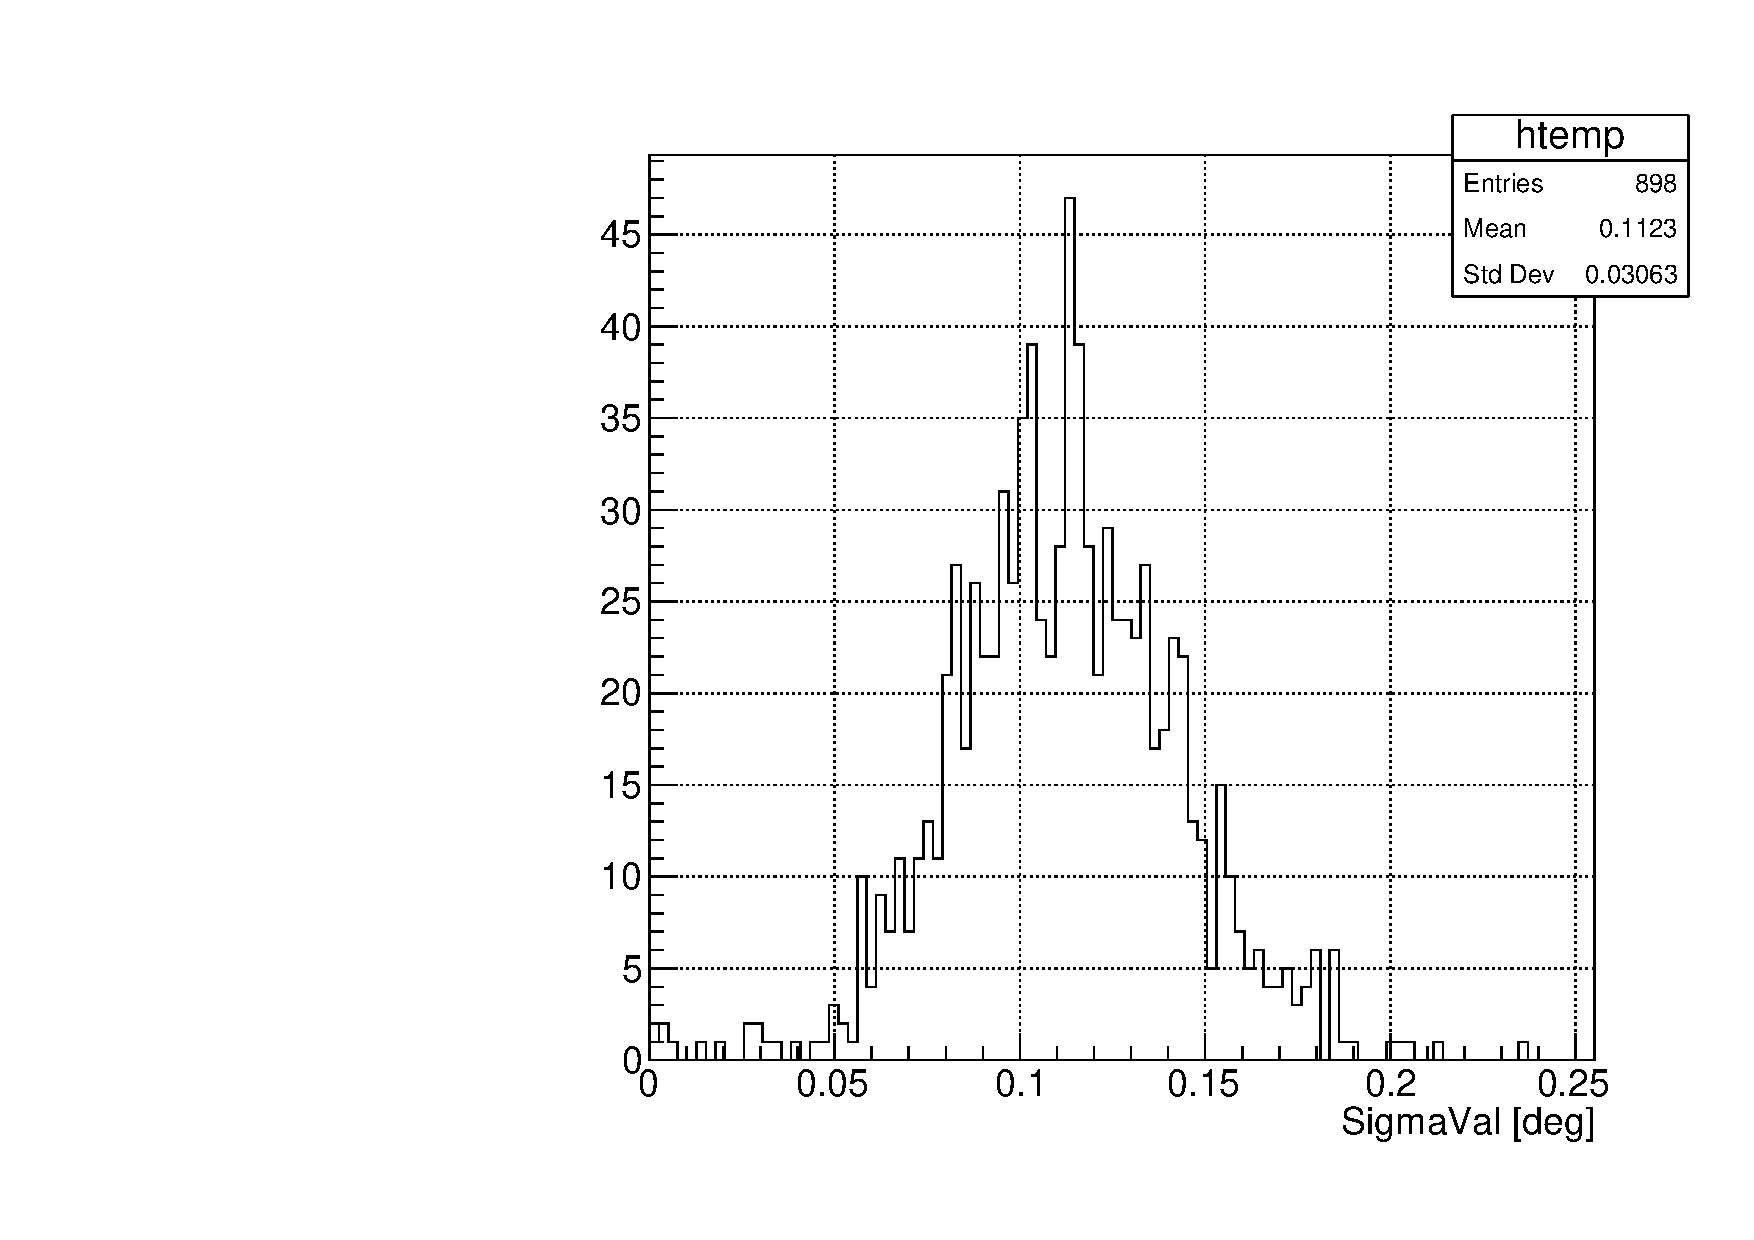
\includegraphics[width=.4\linewidth]{plots/2018/PhiSigmaVal.pdf}
    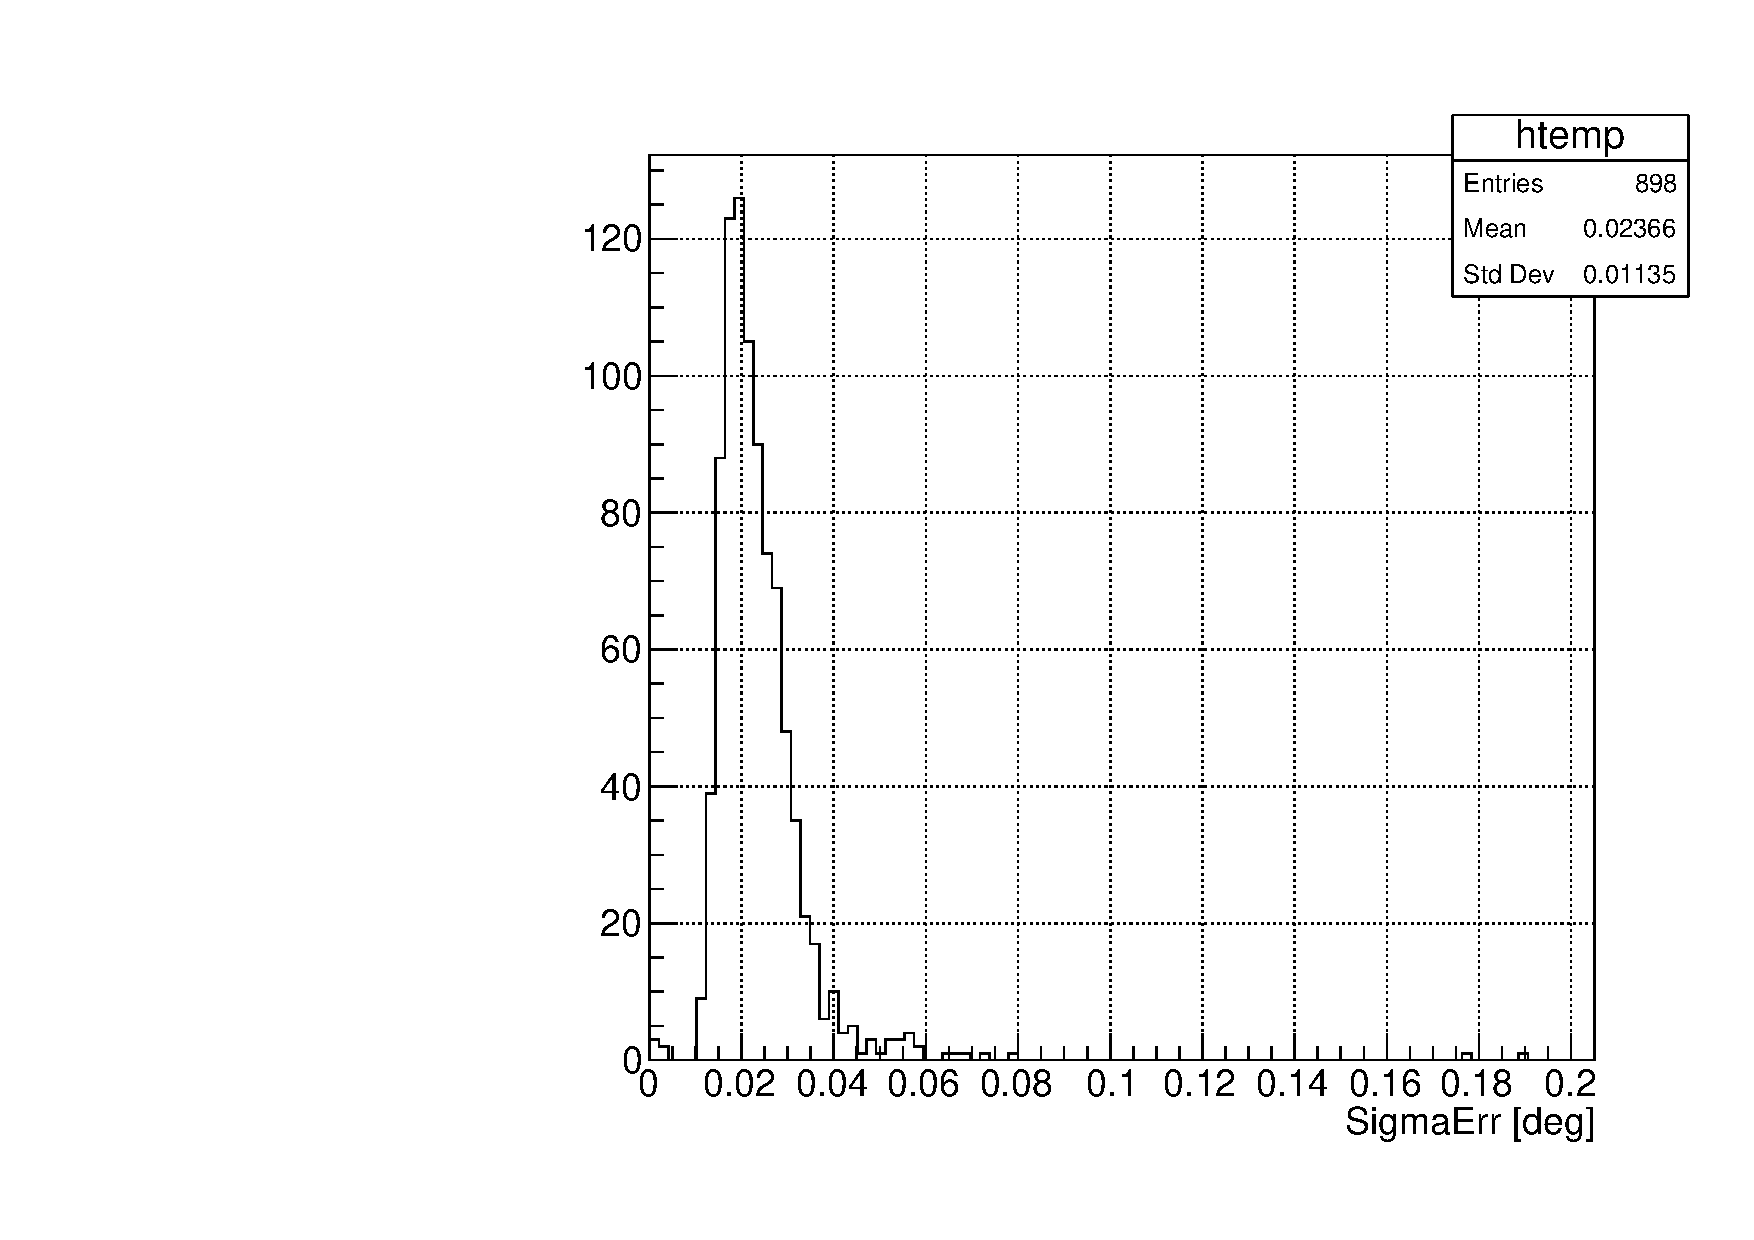
\includegraphics[width=.4\linewidth]{plots/2018/PhiSigmaErr.pdf}\\
    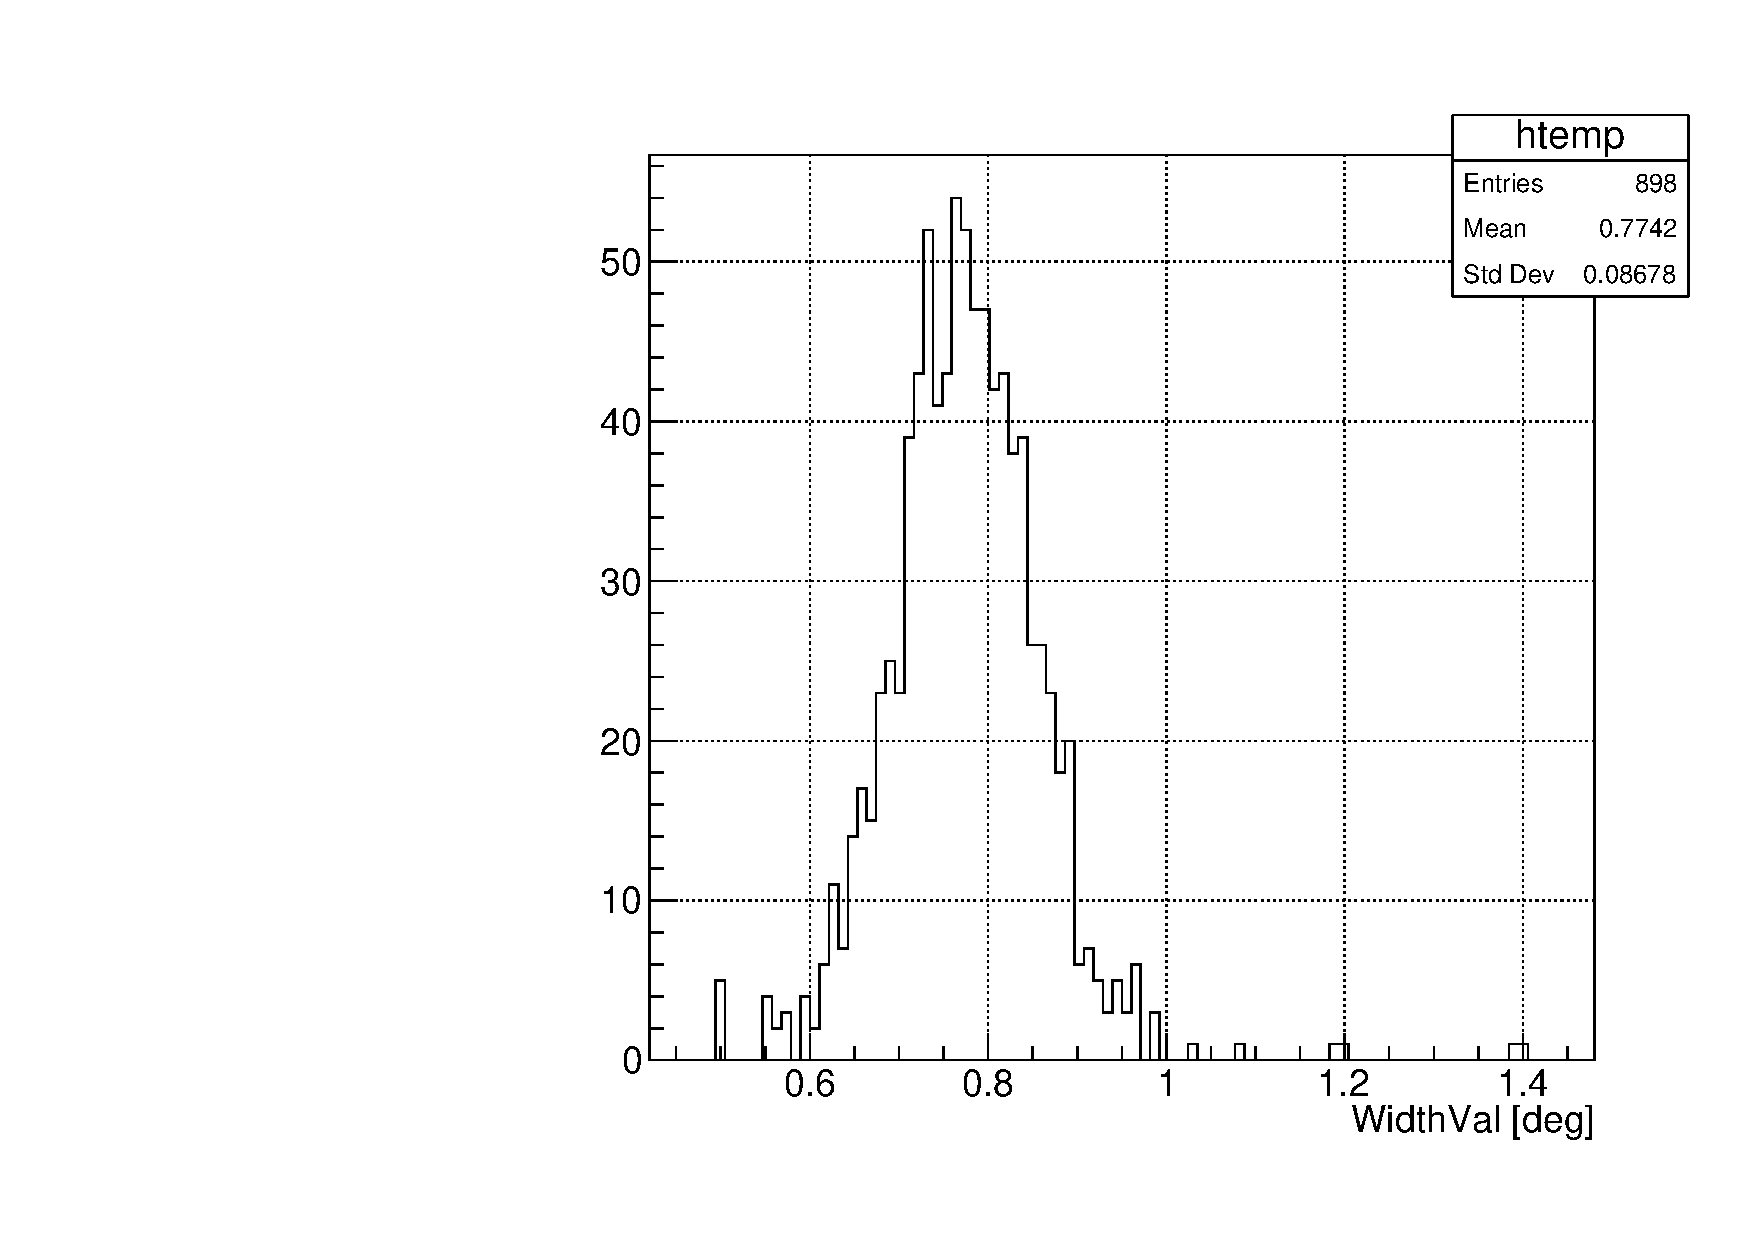
\includegraphics[width=.4\linewidth]{plots/2018/PhiWidthVal.pdf}
    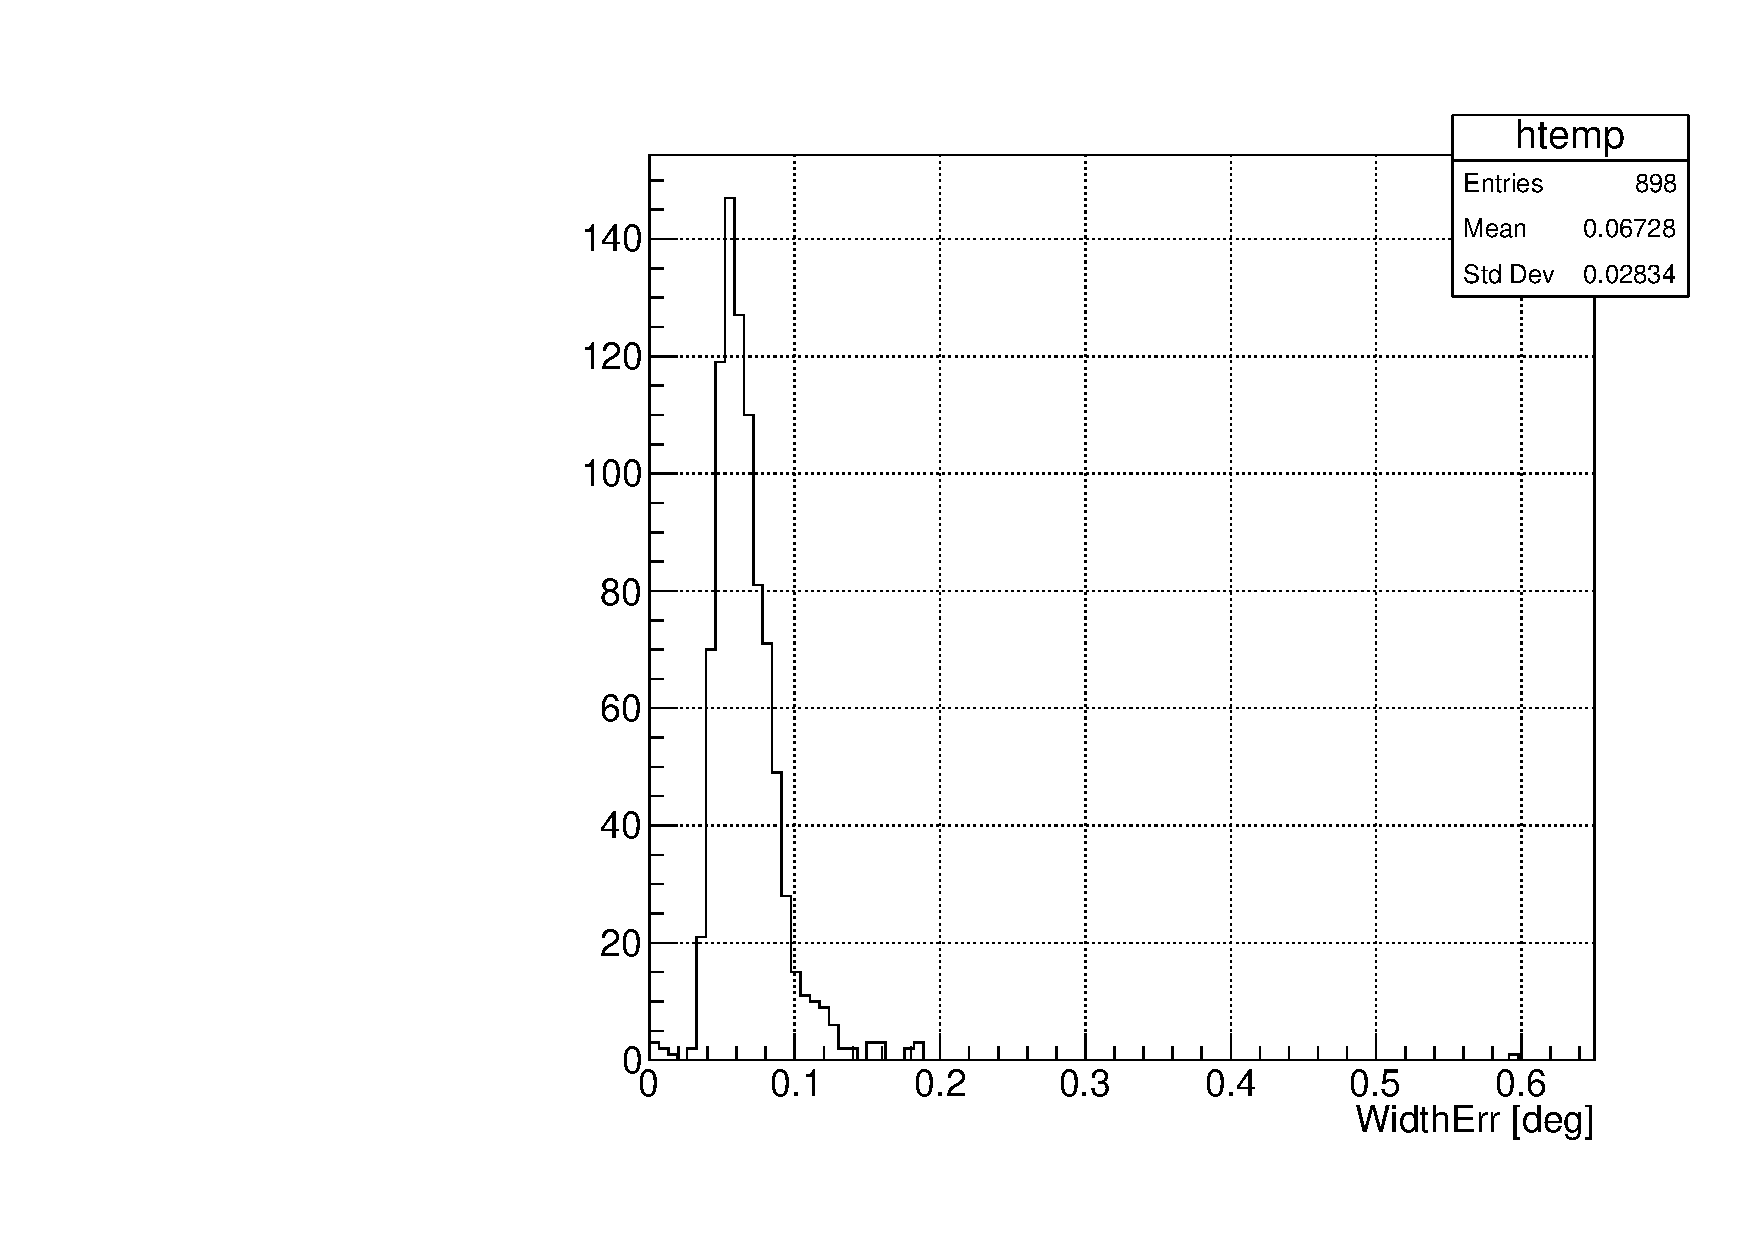
\includegraphics[width=.4\linewidth]{plots/2018/PhiWidthErr.pdf}\\
    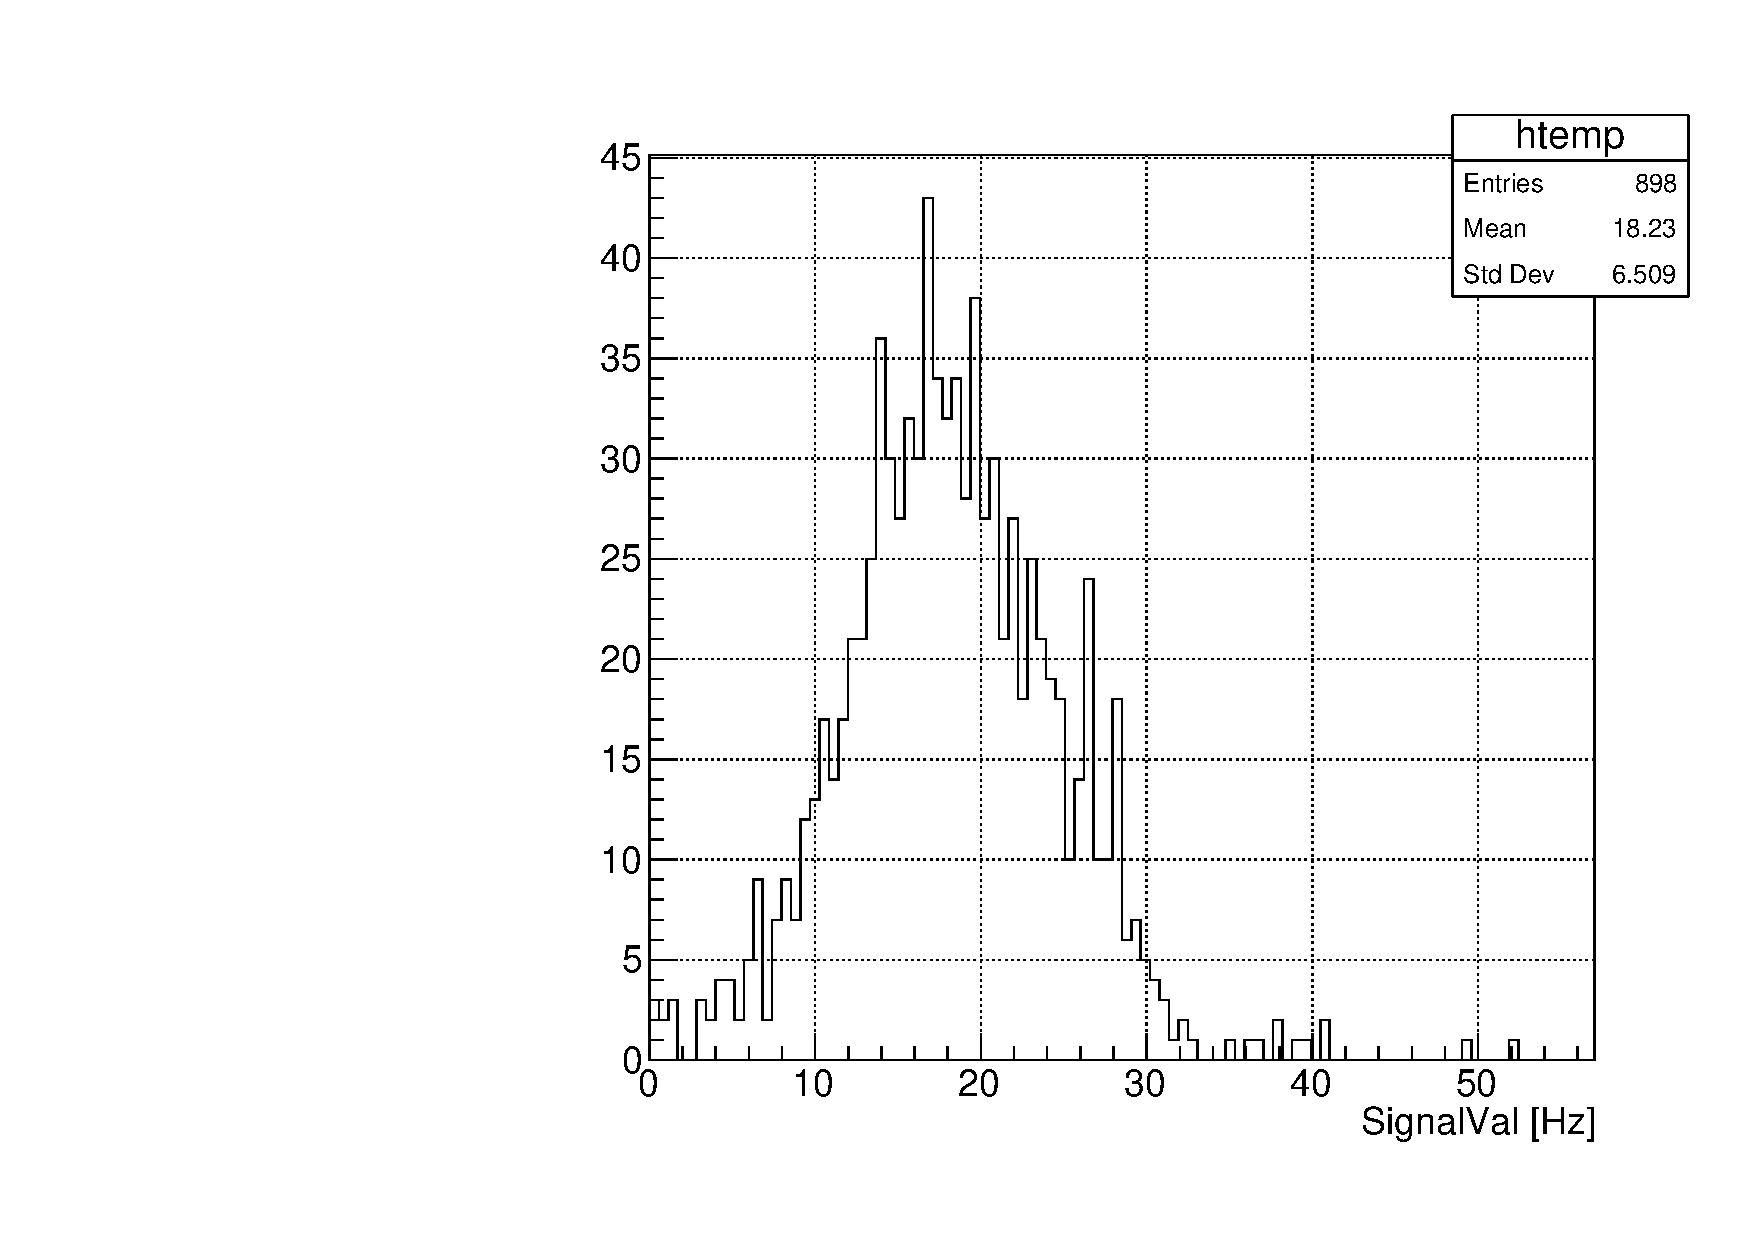
\includegraphics[width=.4\linewidth]{plots/2018/PhiSignalVal.pdf}
    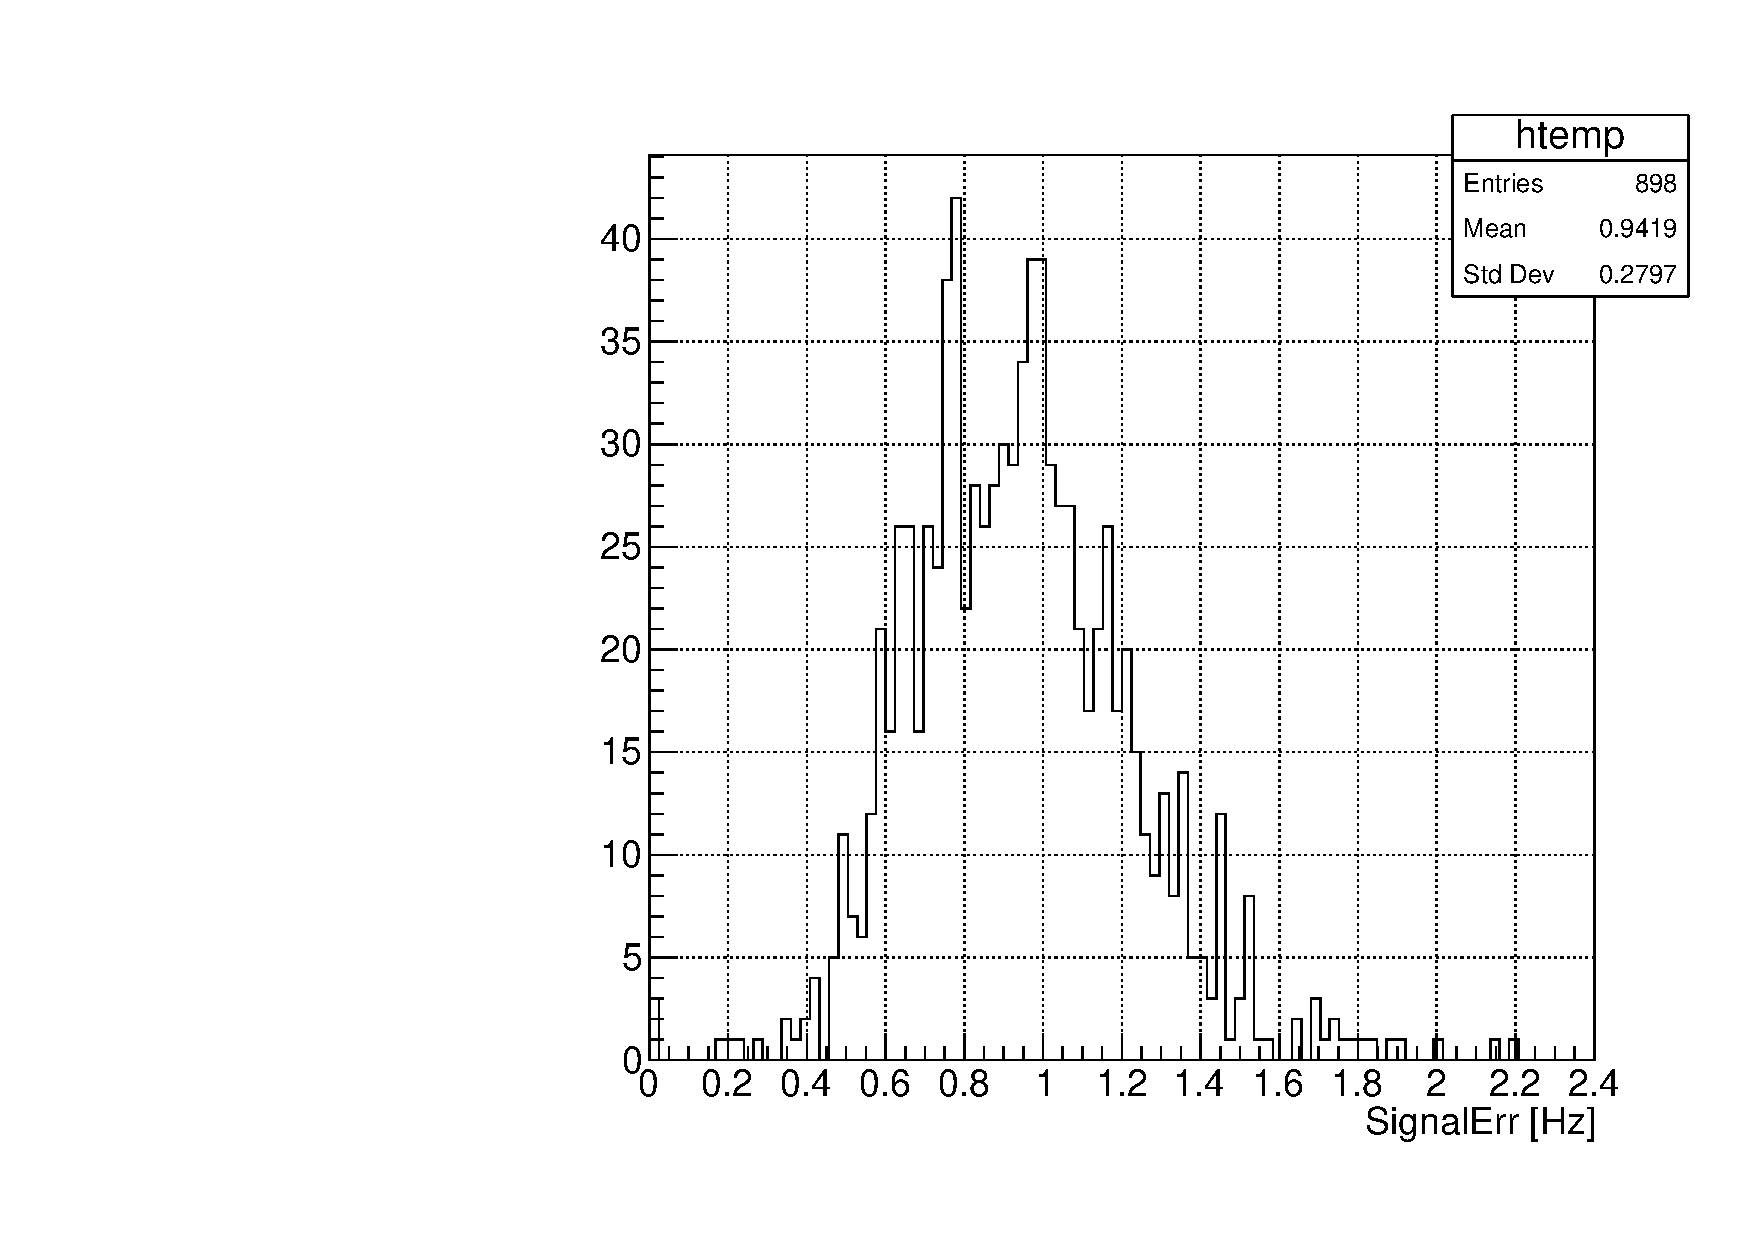
\includegraphics[width=.4\linewidth]{plots/2018/PhiSignalErr.pdf}\\
    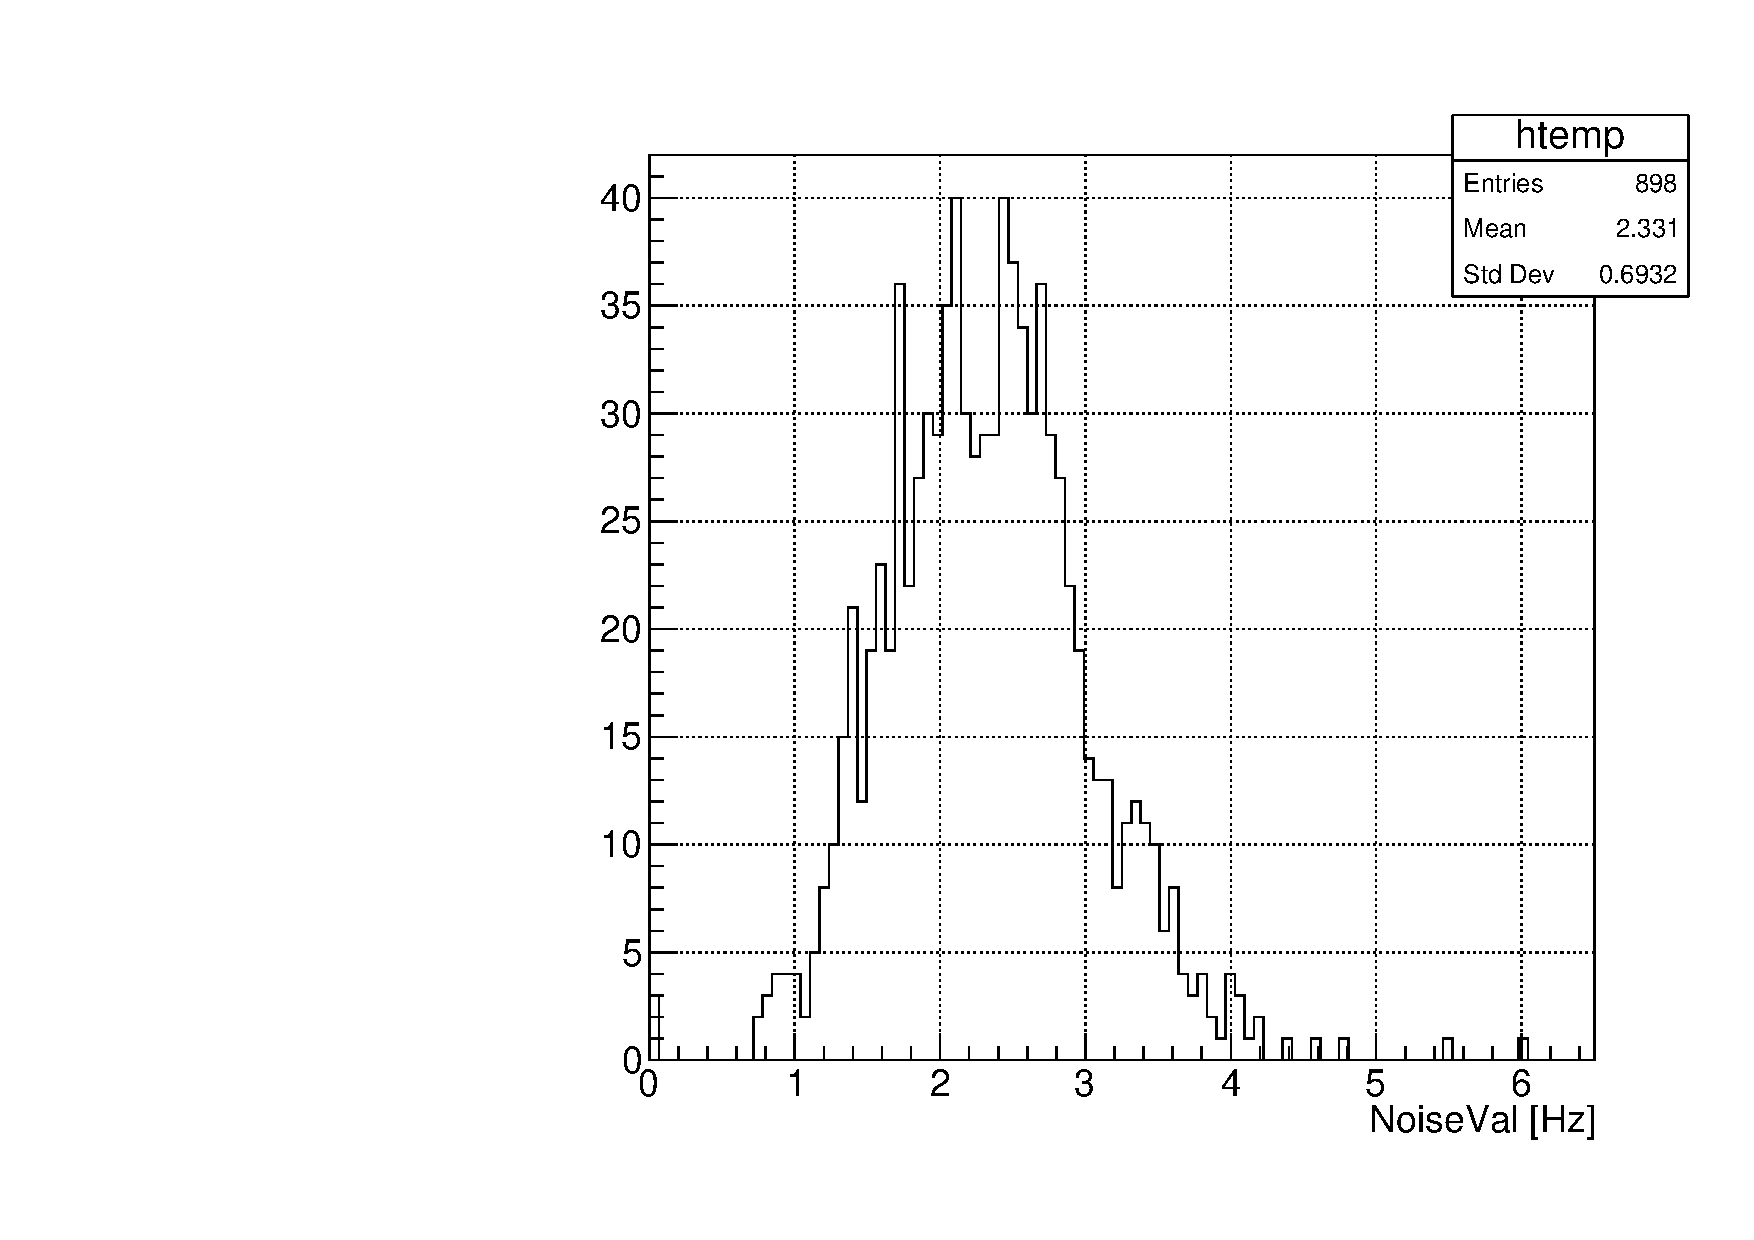
\includegraphics[width=.4\linewidth]{plots/2018/PhiNoiseVal.pdf}
    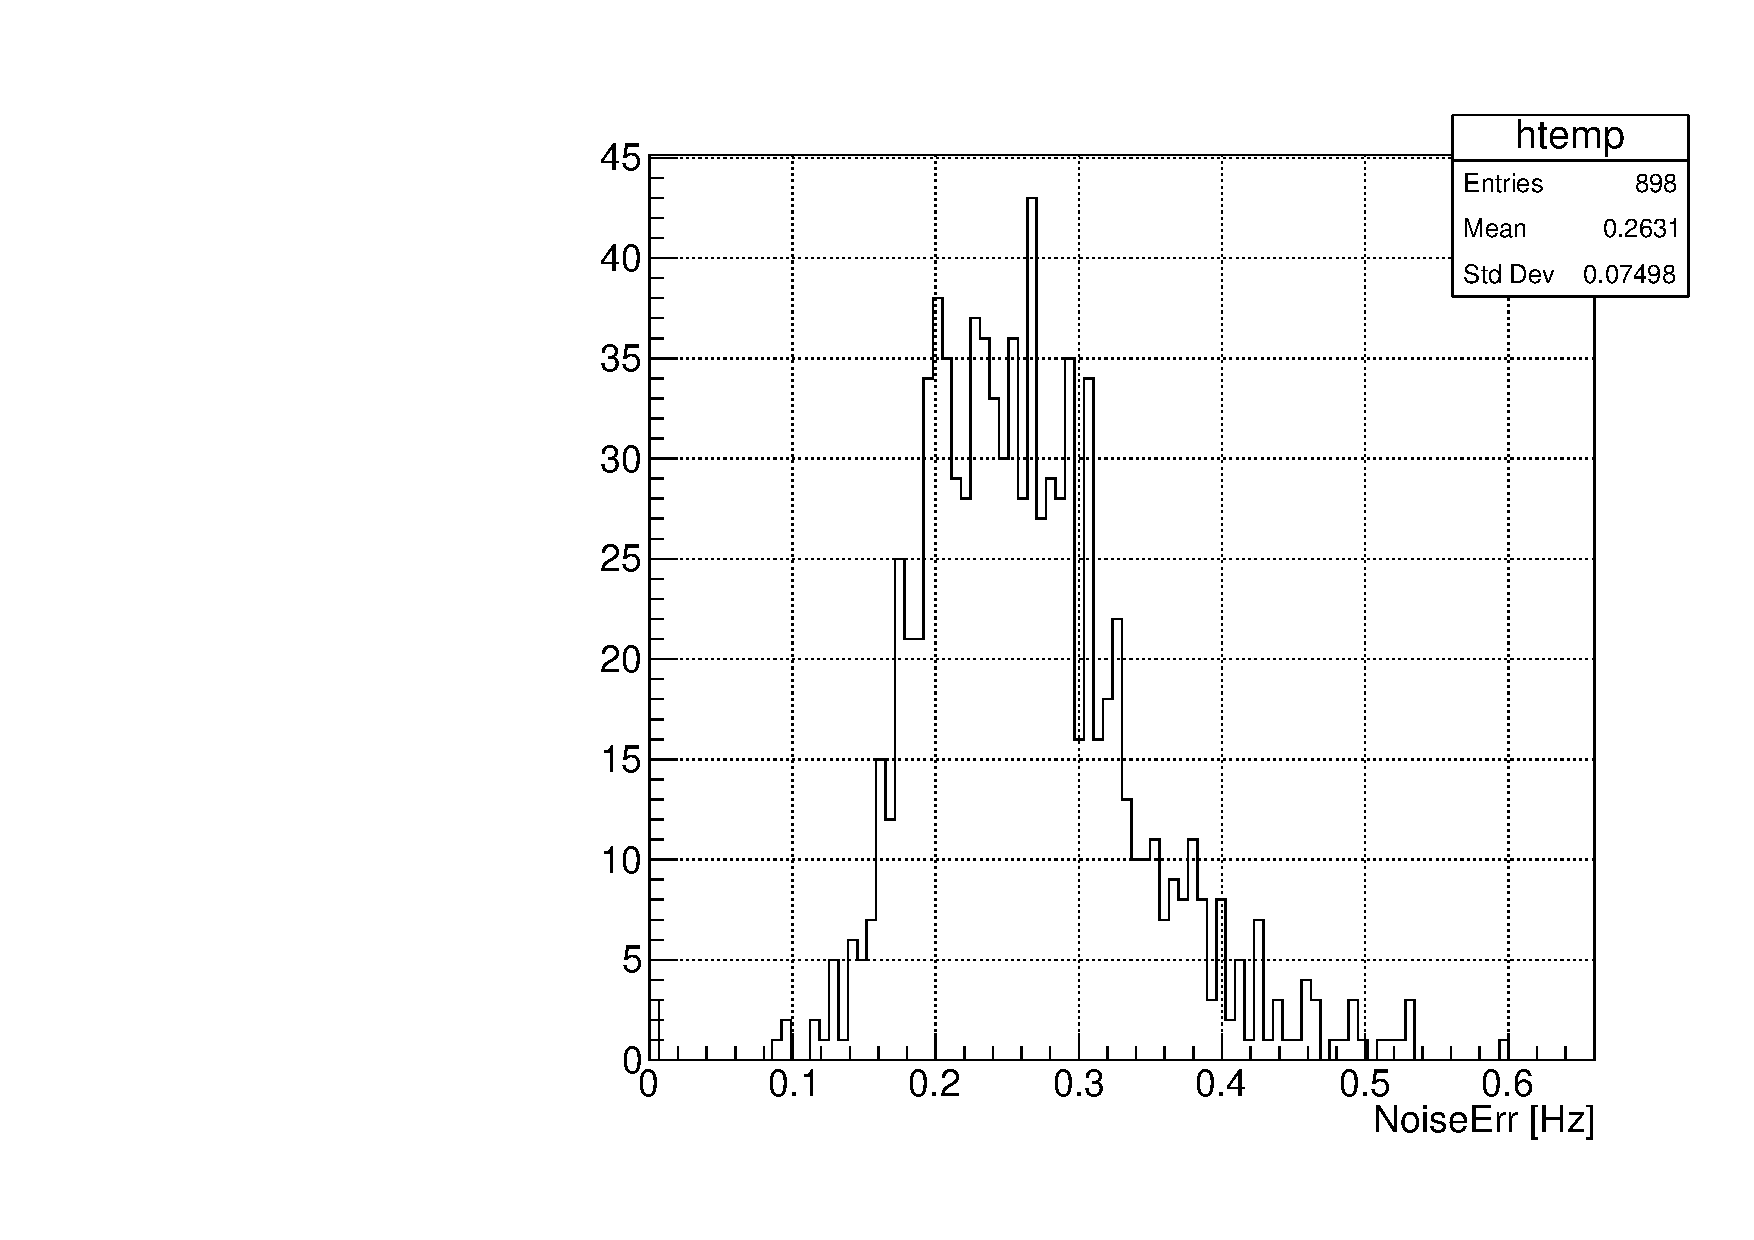
\includegraphics[width=.4\linewidth]{plots/2018/PhiNoiseErr.pdf}
    \caption{Fitted parameter values (left) and errors (right) for $\phi$ position fits.}
    \label{fig:zfitpars}
\end{figure}
